\documentclass[c, 9pt, pdftex, xcolor=table]{beamer}
%\usetheme{CEA}
\usepackage{etex}
\usepackage{tabularx}
\usepackage{multirow}
\usepackage{gensymb}
\usepackage[utf8]{inputenc}
%\usepackage[french]{babel}
\usepackage[english]{babel}
%\usepackage{bibentry}
%\nobibliography*
\usepackage[style=alphabetic,citestyle=alphabetic, sorting=nty, backend=bibtex]{biblatex}
\bibliography{../all_my_bib}
\usepackage{listings}
\usepackage{sty/lstlangarm}
%\usepackage{subfig}
\usepackage{verbatim}
\usepackage{sty/stylebeamerCEA}
\usepackage{amsmath}
\usepackage{amssymb}
\usepackage{amsfonts}
\usepackage{amsthm}
\usepackage{siunitx}
\usepackage[table]{xcolor}
\usepackage{graphicx}
\usepackage{array}
\usepackage{subfigure}
%\usepackage{pgfgantt}
\usepackage[normalem]{ulem}
\usepackage[rightcaption]{sidecap}
%\usepackage[export]{adjustbox}
\setbeamertemplate{bibliography item}{\insertbiblabel}
% Permet d'afficher le bandeau CONFIDENTIEL CESTI
\def\bandeauconf#1{
    \textcolor{#1}{
        \renewcommand{\arraystretch}{1.6}
        \begin{tabularx}{\linewidth}{!{\vrule width 1pt}@{}XcX!{\vrule width 1pt}}
        \noalign{\hrule height 1pt}
        &  \textbf{Diffusion restreinte CESTI} & \\
            \noalign{\hrule height 1pt}
        \end{tabularx}
    }
}




%\usepackage{movie15}
\definecolor{grey}{rgb}{0.7,0.7,0.7}
\definecolor{gg}{rgb}{0.85,0.85,0.85}
\definecolor{bb}{rgb}{0.4,0.4,0.4}
%Define colors
\definecolor{blue2}{rgb}{0.3,0.7,1}
\definecolor{blue3}{rgb}{0.4,0.75,1}
\definecolor{blue4}{rgb}{0.55,0.8,1}
\definecolor{blue5}{rgb}{0.7,0.85,1}

%define colors by uses
\definecolor{simcolor}{cmyk}{0.683, 0.482, 0, 0.145} % couleur du simulateur
\definecolor{modcolor}{cmyk}{0.119, 0.547, 0, 0.376} % couleur du modele
\definecolor{gencolor}{cmyk}{0, 0.75, 1, 0.2} % couleur du generateur
\definecolor{filecolor}{cmyk}{0, 0.109, 0.271, 0.031} % couleur des entrees/sorties
\definecolor{gramcolor}{cmyk}{0, 0.4, 1, 0} % couleur du module de grammaire
\definecolor{chipcolor}{cmyk}{0, 0.153, 1, 0} % couleur de la chip d'une càp
\definecolor{attackcolor}{cmyk}{0, 0.2, 1, 0} % couleur des attaques

\definecolor{cpucolor}{cmyk}{0,0.492,0.41,0.522} % couleur du processeur
\definecolor{cocolor}{cmyk}{0.5,1,0,0.2} % couleur des coprocesseurs
\definecolor{memcolor}{cmyk}{0.742,0,0.05,0.529} % couleur de la mémoire
\definecolor{buscolor}{cmyk}{0.555,0,0.486,0.427} % couleur du bus de données
\definecolor{circolor}{cmyk}{0,0,0,0.4} % couleur du fond de circuit

\definecolor{trigcolorleft}{HTML}{7ACC29}
\definecolor{trigcolorright}{HTML}{19D1FF}
\definecolor{trigcolorbottom}{HTML}{336680}

\usepackage{tikz}
%\usepackage{pgfgantt}
\usetikzlibrary{mindmap,backgrounds}
\usetikzlibrary{shapes}
\usetikzlibrary{shapes.symbols}
\usetikzlibrary{decorations.pathreplacing}
\usetikzlibrary{decorations.markings}
\usetikzlibrary{arrows}
\usetikzlibrary{patterns}
\usetikzlibrary{calc}
\usetikzlibrary{positioning}
%\usetikzlibrary{chains,positioning,shapes.symbols,fadings,shadows, backgrounds}
\usetikzlibrary{decorations.pathmorphing}
\usetikzlibrary{shapes.callouts}
%\usetikzlibrary{shapes.arrows, shadings}
\usetikzlibrary{decorations.text}
\usetikzlibrary{matrix}
\usetikzlibrary{shapes}
\usetikzlibrary{shapes.symbols}
\usetikzlibrary{decorations.pathreplacing}


% attaques
\def\attaqueasma{\only<1,2,3>{\#00}\only<4>{\colorbox{attackcolor}{\#04}}}
\def\attaqueasmb{\only<1,2,4>{\#04}\only<3>{\colorbox{attackcolor}{\#ff}}}
\def\attaqueasmc{\only<1,3,4>{\textcolor{green!40!black}{JNC} \textcolor{blue}{DO}}\only<2>{\colorbox{attackcolor}{NOP NOP}}}
\def\attaqueca{\only<1,2,3>{0}\only<4>{\colorbox{attackcolor}{4}}}
\def\attaquecb{\only<1,2,4>{4}\only<3>{\colorbox{attackcolor}{-1}}}
\def\attaquecca{\only<1,3,4>{\itshape\color{purple!40!black}// main loop}
\only<2>{\colorbox{attackcolor}{goto ATTACK;}}}
\def\attaqueccb{\only<1,3,4>{\itshape\color{purple!40!black}// The
comparison is successful}
\only<2>{\colorbox{attackcolor}{ATTACK:}}}

% my new commands

%
\newcommand{\sensVar}{z}
\newcommand{\sensRandVar}{Z}
\newcommand{\sensVarSet}{\mathcal{Z}}
\newcommand{\plaintext}{p}
\newcommand{\randPlaintext}{P}
\newcommand{\plaintextSet}{\mathcal{P}}
\newcommand{\targetFunction}{e}


\newcommand{\key}{k}
\newcommand{\randKey}{K}
\newcommand{\keyTest}{k^{\star}}
\newcommand{\keySet}{\mathcal{K}}
\newcommand{\esper}{\mathbb{E}}
\newcommand{\var}{\mathrm{Var}}
\newcommand{\SNR}{\mathrm{SNR}}

\newcommand{\numTraces}[1][z]{N_{#1}}
\newcommand{\numTracesAttack}{N_a}
\newcommand{\sss}[2][z]{\textbf{x}^{#1}_{#2}} % $\sss{i}$ or $\sss[k]{i}$
\newcommand{\sssTest}[2][z]{\textbf{y}^{#1}_{#2}} % $\sssTest{i}$ or $\sssTest[k]{i}$
\newcommand{\SSS}[1][z]{\textbf{X}^{#1}}
\newcommand{\sssSet}{\mathcal{X}}
\newcommand{\SSSTest}[1][z]{\textbf{Y}_{#1}}
\newcommand{\featureSpace}{\mathcal{F}}

\newcommand{\extractor}[2][]{\varepsilon_{#1}(#2)}
\newcommand{\extract}{\varepsilon}
\newcommand{\bestExtractor}{\varepsilon^\star}

\newcommand{\AAlpha}{\boldsymbol\alpha}
\newcommand{\BBeta}{\boldsymbol\beta}
\newcommand{\mumumu}{\boldsymbol\mu}
\newcommand{\mmm}{\textbf{m}}
\newcommand{\mmmX}{\overline{\textbf{x}}}
\newcommand{\mmmXclass}[1][z]{\overline{\textbf{x}}^{#1}}
\newcommand{\mmmY}{\overline{\textbf{y}}}
%\newcommand{\mmmX}[1][z]{{\bf \meanEst{{\textnormal{$(#1)$}}}}}
%\newcommand{\mmmY}[1][z]{{\bf \meanEst{{\textnormal{$(#1)$}}}}}

\newcommand{\MMM}{\textbf{M}}
\newcommand{\MMMclass}[1][z]{\textbf{M}_{#1}}
\newcommand{\MMMT}{\textbf{M}_{\textbf{T}}}
\newcommand{\NNN}{\textbf{N}}
\newcommand{\III}{\textbf{I}}

\newcommand{\mmmXtot}{{\overline{\bf \meanEst{}}}}

\newcommand{\meanNoise}{{\bf \mu}}
\newcommand{\meanEst}[1]{\mathrm{\bf m}_1 #1 }
\newcommand{\varEst}[1]{\mathrm{m}_2(#1)}
\newcommand{\mean}[2][]{\Bbb{E}_{#1}\left(#2\right)}


\newcommand{\xxx}{\textbf{x}}
\newcommand{\XXX}{\textbf{X}}
\newcommand{\yyy}{\textbf{y}}
\newcommand{\YYY}{\textbf{Y}}
\newcommand{\measuresMatrix}{\textbf{M}}
\newcommand{\projectingMatrix}{\textbf{A}}
\newcommand{\info}[1][z]{\boldsymbol{\varphi}({#1})}
\newcommand{\BBB}{\textbf{B}}
\newcommand{\zero}{\mathbf{0}}
\newcommand{\traceLength}{D}
\newcommand{\newTraceLength}{C}

\newcommand{\numPoI}{\# PoI}

\newcommand{\covmat}{\textbf{S}}


\newcommand{\succRate}{\mathrm{SR}}
\newcommand{\memComplexity}{m}
\newcommand{\guessingVector}{\mathrm{\textbf{g}}}
\newcommand{\adversary}{\mathcal{A}}
\newcommand{\attackAlgorithm}{\mathrm{A}}
\newcommand{\guessingEntropy}{\mathrm{GE}}
\newcommand{\threshold}{\beta}


\newcommand{\vectorContribution}[1][k]{\mathrm{\textbf{ELV}}(#1)}
\newcommand{\varianceInPoints}[2][n]{\mathrm{H}_{#1}(#2)}
\newcommand{\coupleSet}{\mathbb{J}}

\newcommand{\prob}{\mathrm{Pr}}

\newcommand{\SW}{\textbf{S}_{\textbf{W}}}
\newcommand{\SB}{\textbf{S}_{\textbf{B}}}
\newcommand{\ST}{\textbf{S}_{\textbf{T}}}

\newcommand{\vvv}{\textbf{v}}

\newcommand{\EGV}[1]{\mathrm{EGV(#1)}}
\newcommand{\ELV}{\mathrm{ELV}}

\newcommand{\nununu}{\boldsymbol{\nu}}
\newcommand{\NPoI}{N}



%%%%%


\def\firstcircle{(0,0) circle (2.4cm)}

\def\secondcircle{(45:1.8cm) circle (2.4cm)}
\def\thirdcircle{(0:2.4cm) circle (2.4cm)}

\graphicspath{{figs/}}

% itemizecommands
\def\itemyes{
\includegraphics[width=0.4cm]{../img/yes}}
\def\itemno{
\includegraphics[width=0.4cm]{../img/no}}

% backup commands
\newcommand{\backupbegin}{
   \newcounter{framenumberappendix}
   \setcounter{framenumberappendix}{\value{framenumber}}
}
\newcommand{\backupend}{
   \addtocounter{framenumberappendix}{-\value{framenumber}}
   \addtocounter{framenumber}{\value{framenumberappendix}} 
}

%%%% CONFIGURATION PAQUETAGES %%%%

%% Listings
\lstdefinestyle{customc}{
  belowcaptionskip=1\baselineskip,
  breaklines=true,
  frame=L,
  xleftmargin=\parindent,
  language=C,
  showstringspaces=false,
  basicstyle=\scriptsize\ttfamily,
  keywordstyle=\bfseries\color{green!40!black},
  commentstyle=\itshape\color{purple!40!black},
  identifierstyle=\color{blue},
  stringstyle=\color{orange},
}

\lstdefinestyle{customasm}{
  belowcaptionskip=1\baselineskip,
  frame=L,
  xleftmargin=\parindent,
  language=[x86masm]Assembler,
  basicstyle=\tiny\ttfamily,
  commentstyle=\itshape\color{purple!40!black},
  morecomment=[l]{//},
  morekeywords={SUBB},
}

\lstset{ numbers=left, tabsize=3, frame=single, numberstyle=\ttfamily,
basicstyle=\footnotesize, style=customc,
           captionpos=b, % sets the caption position to bottom
               extendedchars=false, % for babel compatibility
}

\setbeamertemplate{section in toc shaded}[default][50]
\AtBeginSection[]
{
  \frame<handout:0>
  {
    \frametitle{Contents}
    \tableofcontents[sectionstyle=show/shaded,
    subsectionstyle=show/show/shaded, subsubsectionstyle=show/show/show/shaded]
  }
}

\def\etal{\textit{et al.} }
\newcommand {\ie}{{\em i.e.} }
\def\eg{\textit{e.g.} }
\def\via{\textit{via} }
 
%define colors by uses
\definecolor{standardcolor}{rgb}{1.0,1.0,1.0}
\definecolor{simcolor}{cmyk}{0.683, 0.482, 0, 0.145} % couleur du simulateur
\definecolor{modcolor}{cmyk}{0.119, 0.547, 0, 0.376} % couleur du modele
\definecolor{gencolor}{cmyk}{0, 0.75, 1, 0.2} % couleur du generateur
\definecolor{filecolor}{cmyk}{0, 0.109, 0.271, 0.031} % couleur des entrees/sorties
\definecolor{gramcolor}{cmyk}{0, 0.4, 1, 0} % couleur du module de grammaire
\definecolor{chipcolor}{cmyk}{0, 0.153, 1, 0} % couleur de la chip d'une càp
\definecolor{attackcolor}{cmyk}{0, 0.2, 1, 0} % couleur des attaques

\definecolor{cpucolor}{cmyk}{0,0.492,0.41,0.522} % couleur du processeur
\definecolor{cocolor}{cmyk}{0.5,1,0,0.2} % couleur des coprocesseurs
\definecolor{memcolor}{cmyk}{0.742,0,0.05,0.529} % couleur de la mémoire
\definecolor{buscolor}{cmyk}{0.555,0,0.486,0.427} % couleur du bus de données
\definecolor{circolor}{cmyk}{0,0,0,0.4} % couleur du fond de circuit

\newsavebox\chip
\sbox{\chip}{

\begin{tikzpicture}[remember picture,
scale=0.07,
% define styles here
chiplayout/.style={rectangle, draw, fill=chipcolor, rounded corners}
]
\draw[chiplayout] (0, 0) rectangle (9,8);
\draw (3, 0) -- (3, 8);
\draw (3, 2) -- (0, 2);
\draw (3, 4) -- (0, 4);
\draw (3, 6) -- (0, 6);

\draw (6, 0) -- (6, 6);
\draw (6, 2) -- (9, 2);
\draw (6, 4) -- (9, 4);
\draw (6, 6) -- (9, 6);
\end{tikzpicture}
}

\tikzstyle{block} = [rectangle, draw, text width=6em, text centered, rounded corners, minimum height=4em]

\tikzset{middlearrow/.style={
        decoration={markings,
            mark= at position 0.5 with {\arrow{#1}} ,
        },
        postaction={decorate}
    }
}

% tikz block styles
\tikzstyle{decision} =  [diamond, draw, fill=blue!20,
text width=5.5em, text badly centered, node distance=3.2cm, inner
sep=0pt]
\tikzstyle{block} = [rectangle, draw, fill=blue!20,
text width=7.0em, text centered, node distance=3.2cm, rounded corners, minimum height=3em]
\tikzstyle{line} = [draw, -latex']
\tikzstyle{cloud} = [draw, ellipse, fill=red!20, node distance=3cm, 
minimum height=2em]




\title[]{Feature Extraction for Side-Channel Attacks}
%\subtitle{\emph{Analysis and Research of Points of Interest in the Context of Side-Channel Attacks on Smart Card}}

\author{Eleonora Cagli}


\date{05/12/2018, Paris}

\colorlet{codecolor}{standardcolor}
\colorlet{objcolor}{standardcolor}
\colorlet{modelecolor}{standardcolor}
\colorlet{outilscolor}{standardcolor}
\colorlet{mutantscolor}{standardcolor}
\colorlet{oraclecolor}{standardcolor}
\colorlet{attaquescolor}{standardcolor}


% Repartir du pb:

\begin{document}
%\inserttitlepage
% Titleframe
\setbeamertemplate{background
canvas}{
\includegraphics[width=\paperwidth,height=\paperheight]{img-templates/fondceatech}}
\begin{frame}[plain]
	\small
  	\vspace{0.5cm}
	\begin{columns}

	\begin{column}{.36\textwidth}
		\hspace{0.5cm}
	\end{column}

	\begin{column}{.64\textwidth}
		\centering
  		\titlepage
  		\vspace{0.5cm}
		
  		\vspace{0.5cm}
	\end{column}

\end{columns}



\begin{columns}
\begin{column}{\textwidth}
\hfill \emph{PhD Supervisor :} Emmanuel Prouff\\
\hfill \footnotesize{(Safran Identity \& Security)}\\
\hfill \small{\emph{CEA Supervisor :} C\'ecile Dumas\textcolor{white}{}} \\
\hfill \footnotesize{(CEA-Leti Grenoble)}
\end{column}
\end{columns}


\end{frame}

\setbeamertemplate{background canvas}{}



\section{Context}


\begin{frame}
\frametitle{Secure Component and Embedded Cryptography}
\textbf{A piece of hardware with security properties.}\\
\textbf{It usually embeds cryptography to provide security services (authentication, signature, secure messaging with terminals...)}
\begin{columns}
\begin{column}{0.5\textwidth}
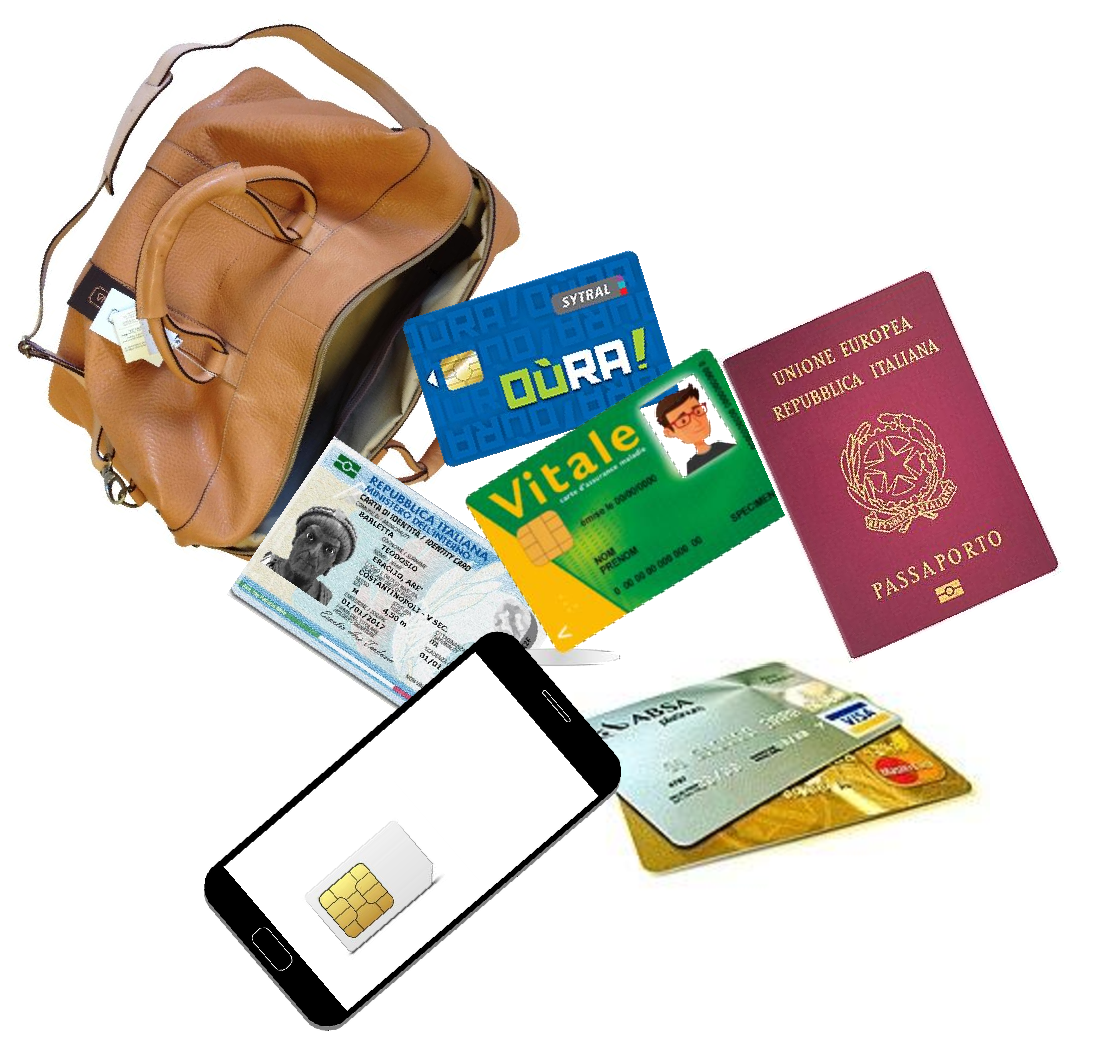
\includegraphics[width = \textwidth]{figures/smartcards.pdf}
\end{column}
\begin{column}{0.5\textwidth}
\begin{itemize}
\item Sensitive applications: ID cards, credit cards, transport cards, health cards, SIM
\item Pervasive aspect: several billion smartcards sold par year
\item Hard to update
\item Hostile environment
\end{itemize}
\end{column}
\end{columns}
$\Rightarrow$ Requires protection against very high-level attacker
\end{frame}

\begin{frame}
\frametitle{Security Certification}
\centering
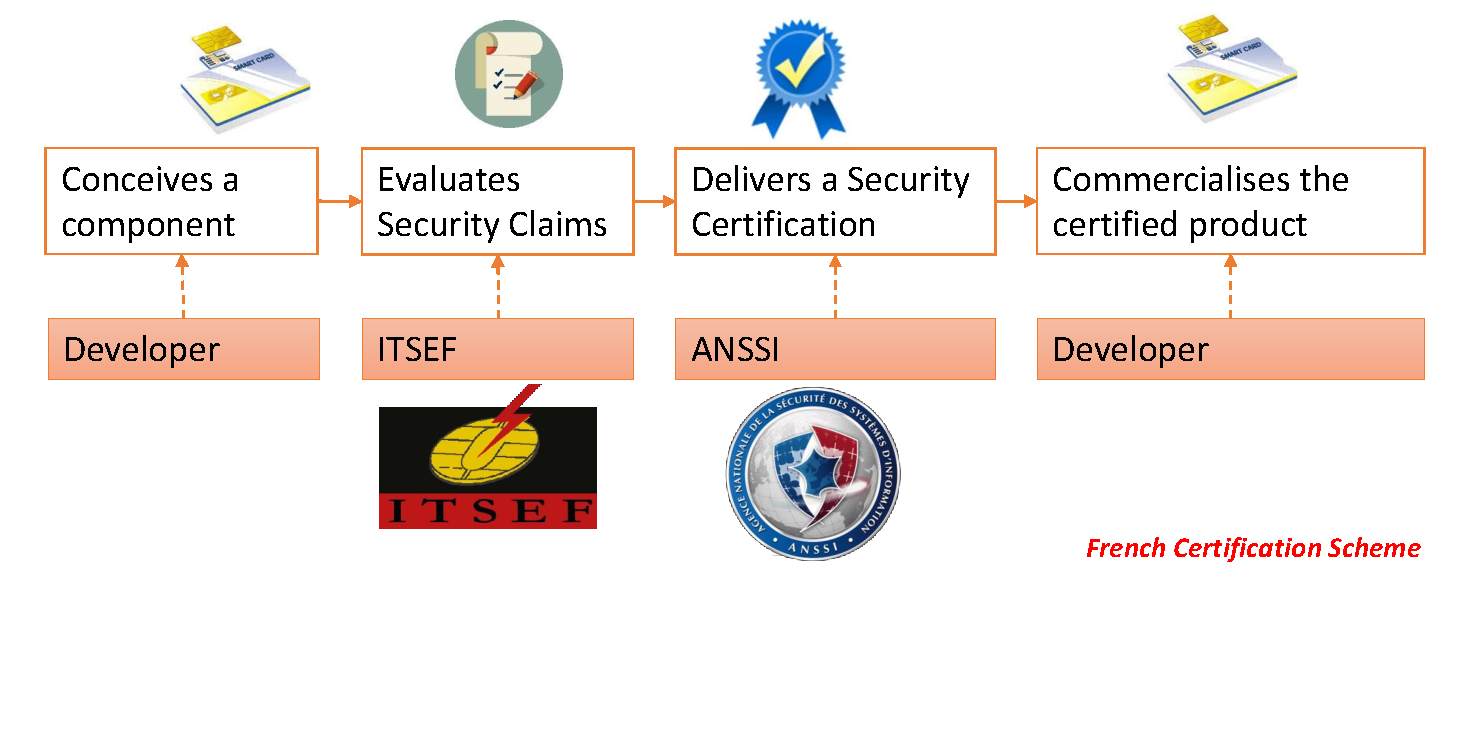
\includegraphics[width = .9\textwidth]{figures/ITSEF_nobody.pdf}
\begin{itemize}
\item Standardized Evaluation (\eg ISO/IEC 15408 - Common Criteria)
\item Assigns an Evaluation Assurance Level (EAL)
\item The evaluator checks the Security Assurance Requirements (SAR), \eg ADV, ALC, AVA, ...
\item AVA: vulnerability assessment (penetration testing $\rightarrow$ attack potential rating)
\end{itemize}
\end{frame}

\begin{frame}
\frametitle{Side-Channel Vulnerability of Embedded Cryptography}
\centering
\scalebox{0.7}{
\begin{tikzpicture}[ ->, node distance = 3cm,
					decoration = {snake,   % <-- added
                    pre length=3pt,post length=7pt,% <-- for better looking of arrow,
                    }]
\node [data] (plaintext){plaintext};
\node [cipher, right of=plaintext] (AES) {\only<1>{AES}\only<2->{
\includegraphics[width = \textwidth]{figures/Computer_Chip-512.png}\\Intermediate Computations}};
\node [data, right of=AES] (ciphertext){ciphertext};
\node [ above right of=AES] (Conso) {Power Consumption};
\node [ below right of=AES] (EM) {Electromagnetic Irradiation};
\node [ above left of=AES] (Time) {Time Duration};
\node [ below left of=AES] (Sound) {Sound Emanation};
\path[draw=blue, very thick, decorate] (AES) -> (Sound);
\path[draw=blue, very thick, decorate] (AES) -> (Time);
\path[draw=blue, very thick, decorate] (AES) -> (Conso);
\path[draw=blue, very thick, decorate] (AES) -> (EM);
\draw [arrow] (plaintext) -- (AES);
\draw [arrow] (AES) -- (ciphertext);
\end{tikzpicture}
}

\begin{columns}
\begin{column}{.5\textwidth}
\textbf{Classical Cryptanalysis}
\begin{itemize}
\item Black box (input, output)
\item Formal attacker model (oracle, knowledge, ...)
\item Computational complexity to perform the attack (\eg $2^{126.1}$ operations to break AES-128 \cite{bogdanov})
\end{itemize}
\end{column}
\begin{column}{.5\textwidth}
\textbf{Side-Channel Cryptanalysis}
\begin{itemize}
\item White box (input, output, side-channel observations of intermediate computations)
\item Attacker with a certain equipment, expertise, knowledge of the embedded device, available time...
\item In Common Criteria: the cotation table of the attack
\end{itemize}
\end{column}
\end{columns}

% con i 5 punti della tesi per definire un attacco
\end{frame}

\begin{frame}
\frametitle{Side-Channel Attacks}
\begin{itemize}
\item TODO: example de trace (square and multiply sans contremesure) $\rightarrow$ attack simple
\item TODO: Schéma avec la puce qui tourne, l'oscillo, les signaux, les hp de clé, le modèle de fuite, le distingueur statistique $r\rightarrow$ attack avancée

\end{itemize}
\end{frame}

\begin{frame}
\frametitle{Side-Channel Attacks Parameters}
\begin{itemize}
\item \textbf{the physical nature of the exploited signals}: \only<1>{power consumption, electromagnetic irradiation}\only<2>{\textcolor{red}{power consumption, electromagnetic irradiation}}, time, sound, temperature, \dots
\item \textbf{the chosen sensitive variable/s} $Z$:
\begin{itemize}
\item $Z = K$ a secret key chunk
\item \only<1>{$Z = f(K,E)$}\only<2>{\textcolor{red}{$Z = f(K,E)$}} a variable depending on a secret key chunk and on a piece of public information
\item an operation (\eg $Z \in \{ square, multiply, \dots\}$)
\item a register 
\item \only<1>{$Z^\prime = \varphi(Z)$}\only<2>{\textcolor{red}{$Z^\prime = \varphi(Z)$}} a non-injective function of any sensitive variable (\eg $f = \mathrm{HW}$ Hamming Weight)
\end{itemize}
\item \textbf{the strategy family}: simple attacks, collision attacks, \only<1>{differential/advanced attacks}\only<2>{\textcolor{red}{differential/advanced attacks}}
\item \textbf{the shape of the attack}: horizontal attacks, vertical attacks
\item \textbf{the attacker knowledge}: \only<1>{profiling}\only<2>{\textcolor{red}{profiling}}, non-profiling attacks
\end{itemize}
\end{frame}




\begin{frame}
\frametitle{Profiling Attacks...Supervised Learning}
\begin{itemize}
\item TODO Figure device under attack and clone device 
\item machine learning \emph{definition}
\item analogy with supervised learning
\end{itemize}

\end{frame}



%\begin{frame}
%\vspace{-15pt}
%\frametitle{Context}
%\begin{block}{Side-Channel Attacks (SCAs)}
%\begin{itemize}
%\item Target: a physical implementations of cryptographic primitives 
%\item Means: observable physical variations (timing information, power consumption, electromagnetic irradiation, etc.)
%\item Goal: retrieve secret data (ex: cryptographic key)
%\end{itemize}
%\end{block}
%
%\begin{block}{Notations}
%\begin{itemize}
%\item Side-channel traces: realizations of a random variable $\XXX \in \mathbb{R}^D$  (column vector)
%\item Target: a \emph{sensitive} variable $Z = f(P,K)\in\sensVarSet$ 
%\end{itemize}
%\end{block}
%\vspace{-5pt}
%\begin{block}{Profiling attack scenario}
%Exploits labelled traces $(\sss[z_i]{i})_{i=1}^N$ to characterize the signals in function of $z_i$.\\
%\emph{"a trace $\sss[z]{}$ belongs to the class $z$"}
%\end{block}
%%\begin{small}
%%\emph{Example: Gaussian Template Attack} 
%%\begin{itemize}
%%\item Profiling phase: estimate the parameters $\{(\mumumu_z,\Sigma_z)\}_{z\in\sensVarSet}$ of multivariate Gaussian distributions
%%\item Attack phase: rank key hypothesis through maximum likelihood
%%\end{itemize}
%%\end{small}
%
%
%
%\end{frame}
%
%
%
%
%%\begin{frame}
%%\vspace{-5pt}
%%\frametitle{Points of Interest}
%%\vspace{-10pt}
%%
%%\begin{block}{Problem}
%%Highly multi-dimensional side-channel traces (algorithm, instruments sampling rate, etc.)\\
%%$\longrightarrow$ affects attack complexity
%%\end{block}
%%
%%\includegraphics[width = 0.4\textwidth]{figures/power_trace.pdf}
%%\only<2>{
%%\includegraphics[width = 0.4\textwidth]{figures/SNR_trace.pdf}
%%}
%%
%%\begin{block}{Which part characterize?}
%%Only (relatively) few points depend on the target: the \emph{Points of Interest (PoIs)}
%%\end{block}
%%
%%\pause
%%\begin{block}{How to find them?}
%%A first answer: statistical tests.\\
%%For example estimating the SNR:
%%\begin{equation}
%%\SNR = \frac{\var(\esper[\XXX\vline Z])}{\esper[\var(\XXX\vline Z)]}
%%\end{equation}
%%\end{block}
%%
%%
%%\end{frame}
%
%
%
%
%\begin{frame}
%\frametitle{Dimensionality Reduction}
%
%\begin{block}{Problem}
%Highly multi-dimensional side-channel traces (algorithm, sampling rate, etc.)\\
%$\longrightarrow$ affect attack complexity
%\end{block}
%
%\begin{block}{Goal}
%Perform a preprocessing via an opportune \emph{extractor} $\extract:\mathbb{R}^D\rightarrow \mathbb{R}^C$ in order to:
%\begin{itemize}
%\item Reduce memory and time complexity (ameliorate the attacks efficiency in terms of required samples)
%\item Enhance contribution of the Points of Interest (PoI, those that depend on the target) to concentrate information over few points (ameliorate the attacks efficiency in terms of required traces)
%\end{itemize}
%\end{block}
%
%%\begin{block}{Extractor}
%%\begin{equation}
%%\extract:\mathbb{R}^D\rightarrow \mathbb{R}^C
%%\end{equation}
%%\end{block}
%
%
%\end{frame}
%
%\begin{frame}
%\frametitle{Literature}
%Two typologies of extractors in literature
%\begin{block}{Selecting Extractors}
%$\extract$ performs a sub-sampling
%\begin{itemize}
%\item Sum of Differences (SOD) \cite{Chari2003}
%\item Signal-to-Noise Ratio (SNR) \cite{mangard2008power}
%\item Sum of Squared $t$-differences (SOST), $t$-test, $F$-test,... \cite{gierlichs2006templates,bar2010improved,choudary2014efficient}
%\end{itemize}
%\end{block}
%
%\begin{block}{Projecting Extractors}
%$\extract(\sss[]{}) = A\sss[]{} \mbox{ with } A \in M_{\mathbb{R}}(\newTraceLength, \traceLength)$
%\begin{itemize}
%\item Principal Component Analysis (PCA) \cite{TAprincipal,Batina2012}
%\item Linear Discriminant Analysis (LDA) \cite{Standaert2008,lessIsMore}
%\end{itemize}
%\end{block}
%
%\end{frame}


\section{State of the Art, Objectives, Contributions}

%\begin{frame}
%\frametitle{Template Attack}
% \begin{textblock}{5}(10,2)
% \important{$\vaLeakVec\in \mathbb{R}^D$\\
%  Curse of dimensionality!}
% \end{textblock}
%\begin{itemize}
%\item Profiling phase (using profiling traces under known $\sensRandVar$)
%\begin{itemize}
%\item \uncover<7->{manage de-synchronization problem}
%\item \uncover<6->{mandatory dimensionality reduction}
%\item \uncover<6->{Gaussian hypothesis \cite{Chari2003}}
%\item \uncover<6->{Variants: \emph{pooled} version \cite{choudary2014efficient}, linear regression \cite{schindler2005stochastic}}
%\item \uncover<2->{estimate \only<2-4>{$\prob[\vaLeakVec|\sensRandVar=\sensVar]$ (generative model)} \only<5-6>{\textcolor{blue}{$\prob[\vaLeakVec|\sensRandVar=\sensVar]$}} \only<7->{\textcolor{blue}{$\prob[\important{\varepsilon(\vaLeakVec)}|\sensRandVar=\sensVar]$}}for each value of $\sensVar$}
%\end{itemize}
%\item Attack phase ($N$ attack traces $\vLeakVec_i$, e.g. with known plaintexts $p_i$)
%
%\only<1-4>{ \begin{itemize}
%\item[] \textcolor{white}{Log-likelihood score for each key hypothesis $k$
%\begin{equation*}
%d_k = \sum_{i=1}^{N}\log \prob[\vaLeakVec=\vLeakVec_i | Z=f(p_i,k)]
%\end{equation*}
%}
%
%\item\textcolor{white}{A-posteriori probability score for each key hypothesis $k$
%\begin{align*}
%\pdf_{\given{\sensRandVar}{  \vaLeakVec = \vLeakVec}}(\sensVar) &= \frac{\pdf_{\given{\vaLeakVec}{\sensRandVar = \sensVar}}(\vLeakVec)\pdf_{\sensRandVar}(\sensVar)} {\pdf_{\vaLeakVec}(\vLeakVec)}\text{Bayes' theorem}\\
%d_{\keyVar} &= \prod_{i=1}^{\nbAttackTraces} \pdf_{\given{\sensRandVar}{\vaLeakVec = \vLeakVec_i}}(\sensFunction(\keyVar,\publicParVar_i) ) \mbox{ ,}
%\end{align*}
%}
%\end{itemize}
%}
%\only<5-6>{\begin{itemize}
%\item Log-likelihood score for each key hypothesis $k$
%\begin{equation*}
%d_k = \sum_{i=1}^{N}\log \textcolor{blue}{\prob[\vaLeakVec=\vLeakVec_i | Z=f(p_i,k)]}
%\end{equation*}
%
%\item A-posteriori probability score for each key hypothesis $k$
%\begin{align*}
%\pdf_{\given{\sensRandVar}{  \vaLeakVec = \vLeakVec}}(\sensVar) &= \frac{\pdf_{\given{\vaLeakVec}{\sensRandVar = \sensVar}}(\vLeakVec)\pdf_{\sensRandVar}(\sensVar)} {\pdf_{\vaLeakVec}(\vLeakVec)} \text{Bayes' theorem}\\
%d_{\keyVar} &= \prod_{i=1}^{\nbAttackTraces} \pdf_{\given{\sensRandVar}{\vaLeakVec = \vLeakVec_i}}(\sensFunction(\keyVar,\publicParVar_i) ) \mbox{ ,}
%\end{align*}
%\end{itemize}
%}
%\only<7->{\begin{itemize}
%\item Log-likelihood score for each key hypothesis $k$
%\begin{equation*}
%d_k = \sum_{i=1}^{N}\log \textcolor{blue}{\prob[\important{\varepsilon(
%\vaLeakVec)}=\important{\varepsilon(
%\vLeakVec_i)} | Z=f(p_i,k)]}
%\end{equation*}
%
%
%\item A-posteriori probability score for each key hypothesis $k$
%\begin{align*}
%\pdf_{\given{\sensRandVar}{  \vaLeakVec = \vLeakVec}}(\sensVar) &= \frac{\pdf_{\given{\vaLeakVec}{\sensRandVar = \sensVar}}(\vLeakVec)\pdf_{\sensRandVar}(\sensVar)} {\pdf_{\vaLeakVec}(\vLeakVec)} \text{Bayes' theorem}\\
%d_{\keyVar} &= \prod_{i=1}^{\nbAttackTraces} \pdf_{\given{\sensRandVar}{\vaLeakVec = \vLeakVec_i}}(\sensFunction(\keyVar,\publicParVar_i) ) \mbox{ ,}
%\end{align*}
%\end{itemize}
%}
%
%\end{itemize}
%
%
%\end{frame}

\begin{frame}
\frametitle{Notations}
\begin{block}{Notations and generalities}
\begin{itemize}
\item Side-channel traces: realizations of a random vector $\vaLeakVec \in \mathbb{R}^D$  
\item $D$ is the number of time samples (or features)
\item Target: a \emph{sensitive} variable $Z = f(\mathrm{plaintext,key})$ in $\sensVarSet = \{\sensVarValue{1}, \dots, \sensVarValue{|\sensVarSet|}\}$
\item each label $\sensVarValue{i}$ identifies a \emph{class}
\end{itemize}
\end{block}
\vspace{-5pt}
\begin{block}{Profiling attack scenario}
\begin{itemize}
\item labelled traces $\setDataTrain = (\vLeakVec_i, z_i)_{i=1}^N$, acquired under known $Z$, to characterise the signals
\item attack traces $\setDataAttack = (\vLeakVec_i, p_i)_{i=1}^{N_a}$ acquired under known plaintext
\end{itemize}
\end{block}
\end{frame}




\begin{frame}
\frametitle{Profiling Attack}
\only<4->{
 \begin{textblock}{5}(10,2)
 \important{$\vaLeakVec\in \mathbb{R}^D$\\
  Curse of dimensionality!}
 \end{textblock}
}

\textbf{Profiling phase}
\begin{itemize}
\uncover<7->{\item manage de-synchronization problem [$\setDataTrain \longrightarrow \rho\colon \mathbb{R}^D\rightarrow\mathbb{R}^D$]}
\uncover<6->{\item mandatory dimensionality reduction [$\setDataTrain \longrightarrow \extract\colon\mathbb{R}^D\rightarrow \mathbb{R}^C$]}
\item estimate
\begin{itemize}
\item $\pdf_{\given{\only<1-5>{\vaLeakVec}\only<6>{\extract{(\vaLeakVec)}}\only<7>{\extract{(\rho(\vaLeakVec)})}}{\sensRandVar = \sensVar}}$\uncover<2->{, $\pdf_{\only<1-5>{\vaLeakVec}\only<6>{\extract{(\vaLeakVec)}}\only<7>{\extract{(\rho(\vaLeakVec)})}}$, $\pdf_{\sensRandVar}$} \uncover<3->{(generative model)}
\uncover<5->{
\begin{itemize}
\item Gaussian hypothesis (\textbf{Template Attack}) \cite{Chari2003}
\item Variants: \emph{pooled} version \cite{choudary2014efficient}, linear regression \cite{schindler2005stochastic}
\end{itemize}
}

\item \uncover<3->{$\pdf_{\given{\sensRandVar}{  \only<1-5>{\vaLeakVec}\only<6>{\extract{(\vaLeakVec)}}\only<7>{\rho(\extract{(\vaLeakVec)})} = \only<1-5>{\vLeakVec}\only<6>{\extract{(\vLeakVec)}}\only<7>{\extract{(\rho(\vLeakVec)})}
}}$ (discriminative model)
}
\end{itemize}
\end{itemize}
\textbf{Attack phase}

\begin{itemize}
\item Log-likelihood score for each key hypothesis $k$
\begin{equation*}
d_k = \prod_{i=1}^{\nbAttackTraces} \pdf_{\given{\only<1-5>{\vaLeakVec}\only<6>{\extract{(\vaLeakVec)}}\only<7>{\extract{(\rho(\vaLeakVec)})}}{\sensRandVar = f(p_i,k)}}(\only<1-5>{\vLeakVec_i}\only<6>{\extract{(\vLeakVec_i)}}\only<7>{\extract{(\rho(\vLeakVec_i)})}
)
%%d_k = \sum_{i=1}^{N}\log \prob[\vaLeakVec=\vLeakVec_i | Z=f(p_i,k)]
\end{equation*}
%
\uncover<2->{
\item A-posteriori probability score for each key hypothesis $k$
\begin{align*}
\pdf_{\given{\sensRandVar}{  \only<1-5>{\vaLeakVec}\only<6>{\extract{(\vaLeakVec)}}\only<7>{\rho(\extract{(\vaLeakVec)})} = \only<1-5>{\vLeakVec}\only<6>{\extract{(\vLeakVec)}}\only<7>{\extract{(\rho(\vLeakVec)})}
}}(\sensVar) &= \frac{\pdf_{\given{\only<1-5>{\vaLeakVec}\only<6>{\extract{(\vaLeakVec)}}\only<7>{\extract{(\rho(\vaLeakVec)})}}{\sensRandVar = \sensVar}}(\only<1-5>{\vLeakVec}\only<6>{\extract{(\vLeakVec)}}\only<7>{\extract{(\rho(\vLeakVec)})}
)\pdf_{\sensRandVar}(\sensVar)} {\pdf_{\only<1-5>{\vaLeakVec}\only<6>{\extract{(\vaLeakVec)}}\only<7>{\extract{(\rho(\vaLeakVec)})}}(\only<1-5>{\vLeakVec}\only<6>{\extract{(\vLeakVec)}}\only<7>{\extract{(\rho(\vLeakVec)})}
)} \text{Bayes' theorem}\\
d_{\keyVar} &= \prod_{i=1}^{\nbAttackTraces} \pdf_{\given{\sensRandVar}{\only<1-5>{\vaLeakVec}\only<6>{\extract{(\vaLeakVec)}}\only<7>{\extract{(\rho(\vaLeakVec)})} = \only<1-5>{\vLeakVec_i}\only<6>{\extract{(\vLeakVec_i)}}\only<7>{\extract{(\rho(\vLeakVec_i)})}
}}(\sensFunction(\keyVar,\publicParVar_i) ) \mbox{ ,}
\end{align*}
}
\end{itemize}

\end{frame}



\begin{frame}
\frametitle{Objectives}
\only<5->{
 \begin{textblock}{5}(5,5)
 \important{DEEP LEARNING}
 \end{textblock}
}
\textbf{Profiling phase}
\begin{itemize}
\item \only<1-3>{\textcolor{grey}{manage de-synchronization problem [$\setDataTrain \longrightarrow \rho\colon \mathbb{R}^D\rightarrow\mathbb{R}^D$]}}\only<4>{\textcolor{red}{manage de-synchronization problem [$\setDataTrain \longrightarrow \rho\colon \mathbb{R}^D\rightarrow\mathbb{R}^D$]}}\only<5->{\textcolor{grey}{manage de-synchronization problem [$\setDataTrain \longrightarrow \rho\colon \mathbb{R}^D\rightarrow\mathbb{R}^D$]}}
\item \only<1-4>{\textcolor{red}{mandatory dimensionality reduction [$\setDataTrain \longrightarrow \extract\colon\mathbb{R}^D\rightarrow \mathbb{R}^C$]}}\only<5->{\textcolor{grey}{mandatory dimensionality reduction [$\setDataTrain \longrightarrow \extract\colon\mathbb{R}^D\rightarrow \mathbb{R}^C$]}}
\item estimate
\begin{itemize}
\item \only<1-4>{$\pdf_{\given{\extract(\vaLeakVec)}{\sensRandVar = \sensVar}}$, $\pdf_{\extract(\vaLeakVec)}$, $\pdf_{\sensRandVar}$ (generative model)}\only<5->{\textcolor{grey}{$\pdf_{\given{\extract(\vaLeakVec)}{\sensRandVar = \sensVar}}$, $\pdf_{\extract(\vaLeakVec)}$, $\pdf_{\sensRandVar}$ (generative model)}}

\begin{itemize}

\item \only<1-4>{Gaussian hypothesis \cite{Chari2003}}\only<5->{
\textcolor{grey}{Gaussian hypothesis \cite{Chari2003}}}
\item \only<1-4>{Variants: \emph{pooled} version \cite{choudary2014efficient}, linear regression \cite{schindler2005stochastic}}
\only<5->{
\textcolor{grey}{Variants: \emph{pooled} version \cite{choudary2014efficient}, linear regression \cite{schindler2005stochastic}}}
%
\end{itemize}

\item \only<1-4>{\textcolor{grey}{$\given{\sensRandVar}{\extract(\vaLeakVec) = \extract(\vLeakVec)}$ (discriminative model)}}\only<5->{\textcolor{red}{$\given{\sensRandVar}{\vaLeakVec = \vLeakVec}$ (discriminative model)}}
\end{itemize}
\end{itemize}
%
\begin{block}{Objectives}
\uncover<2->{
\begin{itemize}
\item Ameliorate the template attack routine by proposing efficient dimensionality reduction techniques
\item \uncover<4->{More generally, ameliorate the profiling attack strategy}
\item \uncover<3->{Consider the presence of most-commonly-implemented SCA countermeasures (masking, hiding)}
\end{itemize}
}
\end{block}
%
\end{frame}



\begin{frame}
\frametitle{Dimensionality Reduction: State of the Art}
\begin{block}{Dimensionality Reduction}
\begin{columns}

\begin{column}{.3\textwidth}
\begin{align*}
\extract \colon & \mathbb{R}^D\rightarrow \mathbb{R}^C\\
& \vLeakVec \mapsto \extract(\vLeakVec)
\end{align*}

\end{column}
\begin{column} {.6\textwidth}
\begin{itemize}
\item Feature selection (Points of Interest selection)
\item Feature extraction
\end{itemize}
\end{column}

\end{columns}
\end{block}
\begin{columns}

\begin{column}{.4\textwidth}
\begin{block}{Feature selection}
$\extract$ performs a sub-sampling
\begin{itemize}
\item SOD \cite{Chari2003}
\item SOST \cite{bar2010improved}
\item SNR \cite{mangard2008power}/ NICV \cite{bhasin2014side}
\item $t$-test, $F$-test,... \cite{gierlichs2006templates,choudary2014efficient}
\end{itemize}
\end{block}
\end{column}

\begin{column}{.6\textwidth}
\only<1>{

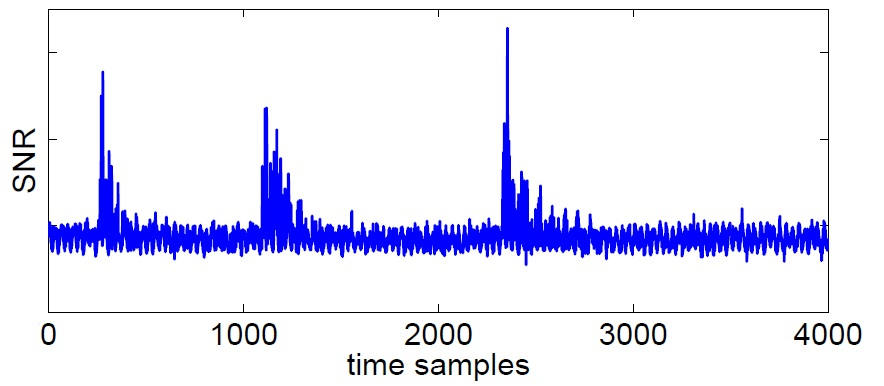
\includegraphics[width = \textwidth]{figures/SNR_1order_new.jpg} 
}
\only<2>{
\begin{block}{Linear feature extraction}
$\extract(\vLeakVec) = A\vLeakVec \mbox{ with } A \in M_{\mathbb{R}}(\newTraceLength, \traceLength)$
\begin{itemize}
\item Principal Component Analysis (PCA) \cite{TAprincipal,Batina2012}
\item Linear Discriminant Analysis (LDA) \cite{Standaert2008,lessIsMore}
\item Projection Pursuits (PP) \cite{PP}
\end{itemize}
\end{block}}
\end{column}
\end{columns}
\end{frame}

\begin{frame}

\frametitle{Contributions}

\begin{itemize}
\item \textbf{Linear Dimensionality Reduction}([CARDIS 2015]): 
\begin{itemize}
\item PCA, choise of components ELV
\item LDA in case of undersampling
\end{itemize}

\item \only<1>{\textbf{Kernel Discriminant Analysis}([CARDIS 2016]): application of an appropriate kernel trick to LDA, in order to manage masking countermeasure}\only<2->{\textcolor{red}{\textbf{Kernel Discriminant Analysis}([CARDIS 2016]): application of an appropriate kernel trick to LDA, in order to manage masking countermeasure}}

\item \only<1>{\textbf{Convolutional Neural Networks}([CHES 2017]) } \only<2->{\textcolor{red}{\textbf{Convolutional Neural Networks}([CHES 2017]) }}:
\begin{itemize}
\item \only<1>{discriminative model by means of neural network classifiers}\only<2->{\textcolor{red}{discriminative model by means of neural network classifiers}}
\item \only<1>{convolutional layers to manage desyncrhonisation (a form of hiding)}\only<2->{\textcolor{red}{convolutional layers to manage desyncrhonisation (a form of hiding)}}
\item \only<1>{Data Augmentation techniques to reduce overfitting}\only<2->{\textcolor{red}{Data Augmentation techniques to reduce overfitting}}
\end{itemize}

\end{itemize}


\end{frame}






%\begin{frame}
%\frametitle{Template Attack} 
%% aprendo des volets per ogni passaggio con riferimenti allo stato dell'arte:
%% templates : likelihood vs MAP ,  cov mats vs pooled , linear regression or not
%% dimensionality reduction : feature selection, feature extraction, masking : masques connus vs unconnus
%% misalignment : re-alignement
%
%\begin{tikzpicture}[ ->, node distance = 3cm,
%					decoration = {snake,   % <-- added
%                    pre length=3pt,post length=7pt,% <-- for better looking of arrow,
%                    }]
%
%\node [data] (db_profiling){
\includegraphics[width = 0.3\textwidth]{figures/database.jpg}\\ Profiling traces};
%\node [data, right of = db_profiling] (db_profiling_realigned){
\includegraphics[width = 0.3\textwidth]{figures/database.jpg}\\ \footnotesize{Realigned profiling traces}};
%\draw[arrow] (db_profiling) -- node[above]{$\rho$} (db_profiling_realigned) ;
%\node[function, above of = db_profiling, yshift=-1cm](realignment){$\rho$};
%\draw[arrow,dashed](db_profiling) -- (realignment);
%\node[function, above of= db_profiling_realigned, yshift=-1cm](extractor){$\varepsilon$};
%\node [data, right of = db_profiling_realigned] (extracted){
\includegraphics[width = 0.3\textwidth]{figures/database.jpg}\\ Profiling traces' features};
%\draw[arrow] (db_profiling_realigned) -- node[above]{$\varepsilon$} (extracted) ;
%\draw[arrow,dashed](db_profiling_realigned) -- (extractor);
%\node[data, right of = extracted, xshift=0.8cm](distributions){\small{$\mathrm{Pr}(\vaLeakVec \mid Z)$}\\
%\small{$\mathrm{Pr}(Z \mid \vaLeakVec)$}};
%\draw[arrow,dashed](extracted) -- node[above]{characterisation} (distributions);
%
%\node[methods, below of= db_profiling, yshift=1cm](realignments){Realignment \cite{nagashima2007dpa,van2011improving,durvaux2012efficient}};
%\node[methods, below of= db_profiling_realigned, yshift=1cm](extraction_methods){Dimensionality reduction};
%\node[methods, below of= extracted, yshift=1cm, align=left](charac_methods){\tiny{
%Template Attack \cite{Chari2003} (generative model, Gaussian hypothesis)\\
%\emph{Pooled} variant \cite{choudary2014efficient}\\
%Stochastic variant \cite{schindler2005stochastic}\\
%Discriminative model
%}};
%\node [data, below of=realignments, yshift=1cm ] (db_attack){
\includegraphics[width = 0.3\textwidth]{figures/database.jpg}\\ Attack traces};
%\node [data, right of = db_attack] (db_attack_realigned){
\includegraphics[width = 0.3\textwidth]{figures/database.jpg}\\ Realigned attack traces};
%\draw[arrow] (db_attack) -- node[above]{$\rho$} (db_attack_realigned) ;
%\node [data, right of = db_attack_realigned] (extracted_attack){
\includegraphics[width = 0.3\textwidth]{figures/database.jpg}\\ Attack traces' features};
%\draw[arrow] (db_attack_realigned) -- node[above]{$\varepsilon$} (extracted_attack) ;
%\node[data, right of = extracted_attack](keys){\footnotesize{$\mathrm{Pr}(K \mid \{ \vaLeakVec_i, P_i \}_{i=1,\dots,N})$}};
%\draw[arrow,dashed](extracted_attack) -- node[above]{inference} (keys);
%
%
%
%\end{tikzpicture}
%\end{frame}
%
%\begin{frame}
%\frametitle{Template Attack} 
%%% aprendo des volets per ogni passaggio con riferimenti allo stato dell'arte:
%%% templates : likelihood vs MAP ,  cov mats vs pooled , linear regression or not
%%% dimensionality reduction : feature selection, feature extraction, masking : masques connus vs unconnus
%%% misalignment : re-alignement
%%
%\begin{tikzpicture}[ ->, node distance = 2.5cm,
%				decoration = {snake,   % <-- added
%                   pre length=3pt,post length=7pt,% <-- for better looking of arrow,
%                   }]
%\uncover<4->{
%\node [data] (db_profiling){
\includegraphics[width = 0.3\textwidth]{figures/database.jpg}\\ Profiling traces};
%\node [data, right of = db_profiling] (db_profiling_realigned){
\includegraphics[width = 0.3\textwidth]{figures/database.jpg}\\ \footnotesize{Realigned profiling traces}};
%\draw[arrow] (db_profiling) -- node[above]{$\rho$} (db_profiling_realigned) ;
%\node[function, above of = db_profiling, yshift=-1cm](realignment){$\rho$};
%\draw[arrow,dashed](db_profiling) -- (realignment);
%\node[function, above of= db_profiling_realigned, yshift=-1cm](extractor){$\varepsilon$};
%\draw[arrow] (db_profiling_realigned) -- node[above]{$\varepsilon$} (extracted) ;
%\draw[arrow,dashed](db_profiling_realigned) -- (extractor);
%}
%
%\node [data, right of = db_profiling_realigned] (extracted){
\includegraphics[width = 0.3\textwidth]{figures/database.jpg}\\ \only<1>{Profiling traces} \only<3->{Profiling traces's features}};
%\node[data, right of = extracted, xshift=0.8cm](distributions){\small{$\mathrm{Pr}(\vaLeakVec \mid Z)$}};
%\draw[arrow,dashed](extracted) -- node[above]{characterisation} (distributions);
%
%\node[methods, below of= db_profiling, yshift=1cm](realignments){Realignment \cite{nagashima2007dpa,van2011improving,durvaux2012efficient}};
%\node[methods, below of= db_profiling_realigned, yshift=1cm](extraction_methods){Dimensionality reduction};
%\node[methods, below of= extracted, yshift=1cm, align=left](charac_methods){\tiny{
%Template Attack \cite{Chari2003} (generative model)\\
%\uncover<3->{\emph{Pooled} variant \cite{choudary2014efficient}\\
%Stochastic variant \cite{schindler2005stochastic}}
%}};
%
%\only<4->{
%\node [data, below of=realignments, yshift=1cm ] (db_attack){
\includegraphics[width = 0.3\textwidth]{figures/database.jpg}\\ Attack traces};
%\node [data, right of = db_attack] (db_attack_realigned){
\includegraphics[width = 0.3\textwidth]{figures/database.jpg}\\ Realigned attack traces};
%\draw[arrow] (db_attack) -- node[above]{$\rho$} (db_attack_realigned) ;
%}
%\node [data, right of = db_attack_realigned] (extracted_attack){
\includegraphics[width = 0.3\textwidth]{figures/database.jpg}\\ \only<1-2>{Attack traces} \only<3->{Attack traces' features}};
%\draw[arrow] (db_attack_realigned) -- node[above]{$\varepsilon$} (extracted_attack) ;
%\node[data, right of = extracted_attack](keys){Maximum Likelihood or Maximum A Posteriori};
%\draw[arrow,dashed](extracted_attack) -- node[above]{inference} (keys);
%
%
%
%\end{tikzpicture}
%\end{frame}
%
%
%\begin{frame}
%\frametitle{Projecting Extractors: PCA and LDA}
%\begin{figure}
%\centering{
%\resizebox{11cm}{!}
%{
%\begin{tikzpicture}[remember picture,
%    scale=0.50,
%    % Define styles here
%    every node/.style={transform shape}
%    block/.style={
%        rectangle,
%        draw,
%        text centered,
%        rounded corners
%        },
%    data/.style={
%        trapezium,
%        trapezium left angle=60,
%        trapezium right angle=120,
%        draw
%        },
%    component/.style={
%        circle,
%        draw
%        },
%    output/.style={
%        tape,
%        tape bend top=none,
%        draw
%        },
%    edge/.style={
%        ->,
%        >=stealth,
%        thick
%        }
%    ]
%
%    % Place nodes
%    \node[inner sep=0pt] (genericTrace) at (0,-0)
%    {\includegraphics[width=0.8\textwidth]{figures/genericTrace.pdf} };
%    \node [above=0.1cm of genericTrace] {Rough Trace};
%    \node [block, below left=0.8cm of genericTrace] (PCA) {\begin{Large}PCA\end{Large}};
%    \node [block, below right=0.8cm of genericTrace] (LDA) {\begin{Large}LDA\end{Large}};
%    \node [below=1.5cm of genericTrace](puntini) {\begin{Large}$\dots$\end{Large}};
%    \node [component, left=0.5cm of puntini](PC2) {\begin{Large}$\AAlpha_2$\end{Large}};
%    \node [component, left=0.5cm of PC2](PC1) {\begin{Large}$\AAlpha_1$\end{Large}};
%    \node [component, right=0.25cm of puntini](PCC) {\begin{Large}$\AAlpha_C$\end{Large}};
%   \node [right=0.25cm of PCC](puntini2) {\begin{Large}$\dots$\end{Large}};
%    \node [component, right=0.15cm of puntini2](PCr) {\begin{Large}$\AAlpha_r$\end{Large}};
%    %\draw[thick, black,decorate,decoration={brace,amplitude=10pt}](PC1.north) -- (PCr.north);
%    \draw(PC1.north)  to [bend left=15] (PCr.north);
%    
%    
%    \draw[->, shorten >=20pt] (PCA.north) node[above=0.4cm] {Principal Components (PCs)} to [bend left] (PC2.north) ;
%     \draw[->,shorten >=25pt] (LDA.north)  node[above=0.35cm] {Discriminant Components (DCs)} to [bend right] (puntini2.north);
%     
%    \only<2>{ 
%    \node [data, below=1cm of puntini](formula1) {\begin{Large}$\sum_{j=1}^D\AAlpha_1[j]\textbf{x}[j]$\end{Large}};
%    \node [left=0.5cm of formula1] {Linear Combination / Projection};
%    \node [below=0.5cm of formula1] (compressed1)
%    	{\includegraphics[width=0.5\textwidth]{figures/compressed1.pdf} }; 
%    	\node[right=0.1cm of compressed1]{Reduced Trace}; 
%	\draw[-, red, thick, shorten >=6pt, shorten <=-6pt](genericTrace.south) to (PC1.north);
%	\draw[-, red, thick, shorten >=6pt, shorten <= 6pt](PC1.south) to (formula1.north);
%	\draw[-, red, thick, shorten <= 2pt, shorten >=-5pt](formula1.south) to (compressed1.north);
%}
%    
%        \only<3>{ 
%        \node [data, below=1cm of puntini](formula2) {\begin{Large}$\sum_{j=1}^D\AAlpha_2[j]\textbf{x}				[j]$\end{Large}};
%    \node [left=0.5cm of formula2] {Linear Combination / Projection};
%    \node [below=0.5cm of formula2] (compressed2)
%    	{\includegraphics[width=0.5\textwidth]{figures/compressed2.pdf} };  
%    	\node[right=0.1cm of compressed2]{Reduced Trace};
%	\draw[-, red, thick, shorten >=6pt, shorten <=-6pt](genericTrace.south) to (PC2.north);
%	\draw[-, red, thick, shorten >=6pt, shorten <= 6pt](PC2.south) to (formula1.north);
%	\draw[-, red, thick, shorten <= 2pt, shorten >=-5pt](formula2.south) to (compressed2.north);
%}
%
% \uncover<4>{ 
%        \node [data, below=1cm of puntini](formulaC) {\begin{Large}$\sum_{j=1}^D\AAlpha_C[j]\textbf{x}				[j]$\end{Large}};
%    \node [left=0.5cm of formulaC] {Linear Combination / Projection};
%    \node [below=0.5cm of formulaC] (compressedC)
%    	{\includegraphics[width=0.5\textwidth]{figures/compressedAll.pdf} }; 
%    \node[right=0.1cm of compressedC]{Reduced Trace};
%	\draw[-, red, thick, shorten >=6pt, shorten <=-6pt](genericTrace.south) to (PCC.north);
%	\draw[-, red, thick, shorten >=6pt, shorten <= 6pt](PCC.south) to (formulaC.north);
%	\draw[-, red, thick, shorten <= 2pt, shorten >=-5pt](formulaC.south) to (compressedC.north);
%}
%    
%     
%     
%
%\end{tikzpicture}
%}
%}
%
%\end{figure}
%\end{frame}



\begin{frame}
\frametitle{PCA and LDA}
\only<1>{
\vspace{-50pt}
\begin{block}{Standard PCA}
\begin{itemize}
\item maximizing data variance
\item not exploiting sensitive variable knowledge
\end{itemize}
\end{block}
\vfill
}
\only<2->{
\begin{block}{Class-oriented PCA}
\begin{itemize}
\item\only<2->{eigenvector research}
\item \only<2->{maximizing inter-class variance}
\item \only<3->{not minimizing the intra-class variance}
\item \only<4->{easily and accurately computable (no matrix inversions)}
\item \only<5->{\textcolor{red}{components selection issue} (disagreement between theory and experience)$\longrightarrow $ ELV selection tool [CARDIS 2015]}
\end{itemize}
\end{block}
}
\only<2-5>{
\begin{block}{LDA}
\begin{itemize}
\item\only<2-5>{eigenvector research}
\item \only<2-5>{maximizing inter-class variance while minimizing intra-class variance (no loss of information under some leakage model \cite{lessIsMore})}
\item \only<4-5> {not easily computable (asking for a matrix inversion)}
\end{itemize}
\end{block}
}



\end{frame}

\begin{frame}
\frametitle{Overview of experimental results of the ELV selection tool}
\begin{block}{Overview of experimental results of the ELV selection tool}
\begin{itemize}
\item large profiling set: PCA performances close to the LDA's if equipped with ELV (and less expensive)
\item small profiling set: LDA efficiency decreases faster than (PCA $+$ ELV)'s \item too small profiling set: LDA unavailable. PCA$+$ELV still efficient
\end{itemize}

\end{block}
\end{frame}

\begin{frame}
\frametitle{Contents}
\begin{itemize}
\item \textcolor{grey}{Introduction to LDA: as a classifier, and as a feature extractor}
\item \important{Introduction to masking countermeasure and Kernel Discriminant Analysis as a feature extractor}
\item Convolutional Neural Networks and Data Augmentation to attack jitter-based countermeasure
\end{itemize}
\end{frame}

%\subsubsection{Components Selection Issue}
%
%\begin{frame} \frametitle{The Problem of Selecting PCA Components}
%
%% state of the art
%% first and sixth PC DPA contest
%\begin{columns}
%\begin{column}{0.1\textwidth}
%\includegraphics[width = \textwidth]{figures/questionmark.jpg} 
%\end{column}
%\begin{column}{0.7\textwidth}
%\begin{block}{}
%{\em How many} PCs and {\em which ones} are sufficient/necessary to reduce the traces size without losing important discriminant information?
%\end{block}
%\end{column}
%\end{columns}
%\vspace{-7pt}
%\begin{block}{Experimental Observation}
%\cite{Batina2012,specht}: the first components sometimes contain no sensitive information; it is worth discarding them.
%\end{block}
%\begin{figure}
%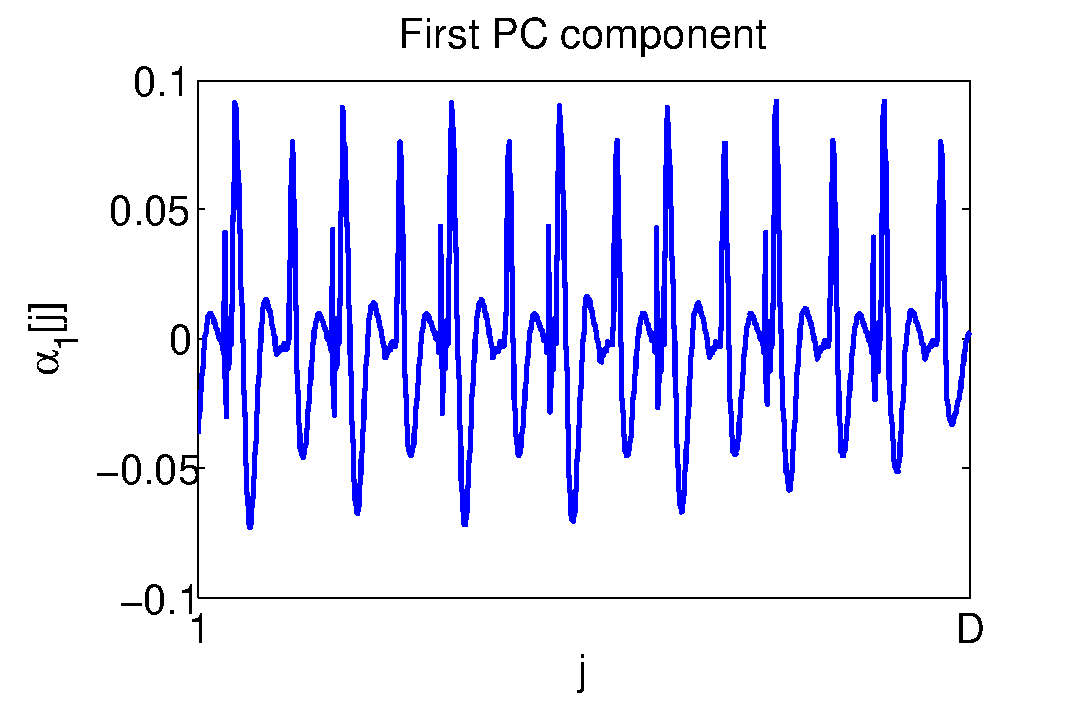
\includegraphics[width=.45\textwidth]{figures/DPAcontestPC1_new.pdf} 
%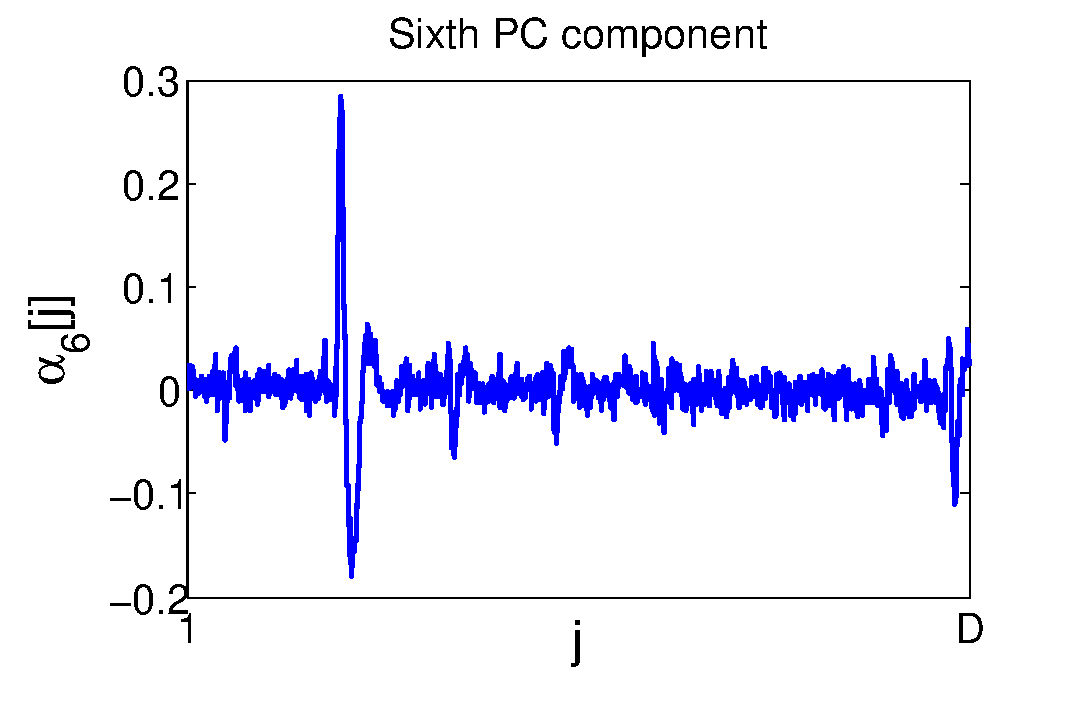
\includegraphics[width=.45\textwidth]{figures/DPAcontestPC6_new.pdf} 
%\caption{First and sixth PCs in DPA contest v4  \cite{DPAcontest} trace set}\label{fig:DPAcontest}
%\end{figure}
%
%
%
%
%
%\end{frame}
%
%
%\begin{frame} \frametitle{The Problem of Selecting PCA Components - EGV, IPR}
%\begin{block}{Explained Global Variance (EGV)}
%$\EGV{\AAlpha_i} = \frac{\lambda_i}{\sum_{k=1}^r \lambda_k}$\\
%\cite{choudaryefficient} : 
%\begin{itemize}
%\item fix a threshold $\beta$
%\item choose the first $C$ components, where $C$ is the minimum integer such that
%\begin{equation*}
%\EGV{\AAlpha_1}+ \EGV{\AAlpha_2}+\dots + \EGV{\AAlpha_C} \geq \beta
%\end{equation*}
%\end{itemize}
%\end{block}
%%\begin{block}{Assumption}
%%Dealing with secured devices, the leaking side-channel information is localised in few points of the acquired trace.
%%\end{block}
%
%\begin{block}{Inverse Participation Ratio (IPR)}
%\cite{SCAclassProbl}: 
%\begin{equation*}
%\mathrm{IPR}(\AAlpha_i) = \sum_{j=1}^\traceLength \AAlpha_i[j]^4 \mbox{ \em (localization score)}
%\end{equation*}
%\end{block}
%\end{frame}


%\begin{frame} \frametitle{The Component Selection Issue}
%
%\begin{columns}
%\begin{column}{0.1\textwidth}
%\includegraphics[width = \textwidth]{figures/questionmark.jpg} 
%\end{column}
%\begin{column}{0.7\textwidth}
%\begin{block}{}
%{\em How many} PCs and {\em which ones} are sufficient/necessary to reduce the traces size without losing important discriminant information? 
%\end{block}
%\end{column}
%\end{columns}
% \only<1>{
% \begin{block}{Theoretically}
%Higher eigenvalues $\longrightarrow$ higher information.
%\end{block}
%\begin{block}{Experimental Observation}
%\cite{Batina2012,specht}: the first components sometimes contain no sensitive information; it is worth discarding them.
%\end{block}
%
%\begin{figure}
%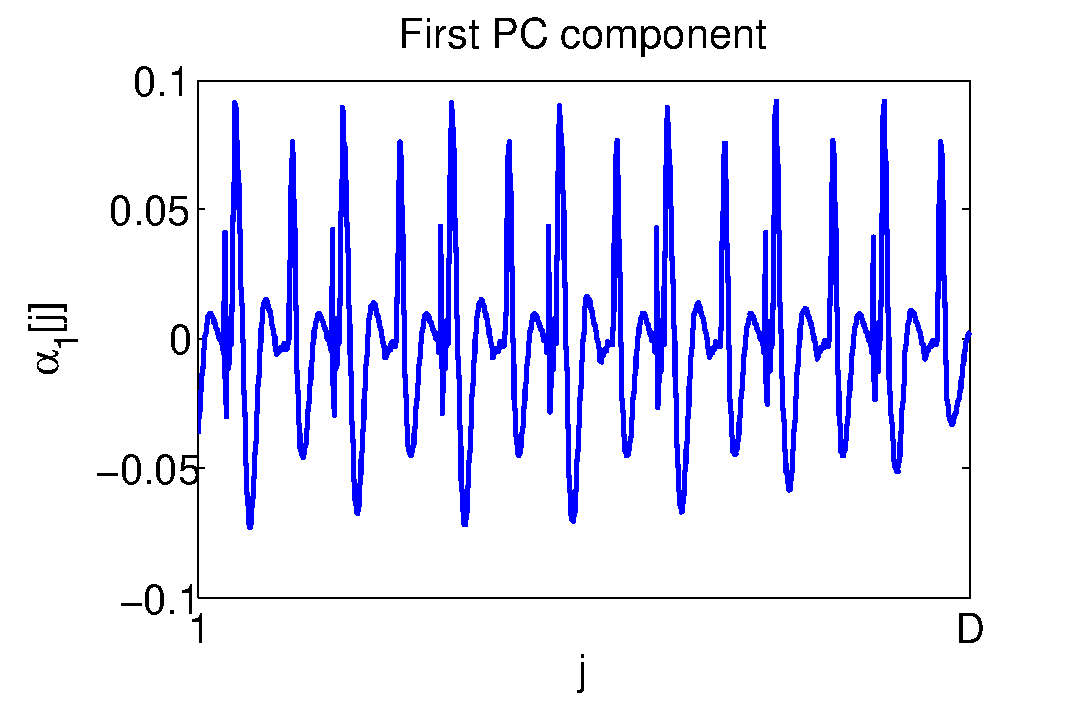
\includegraphics[width=.25\textwidth]{figures/DPAcontestPC1_new.pdf} 
%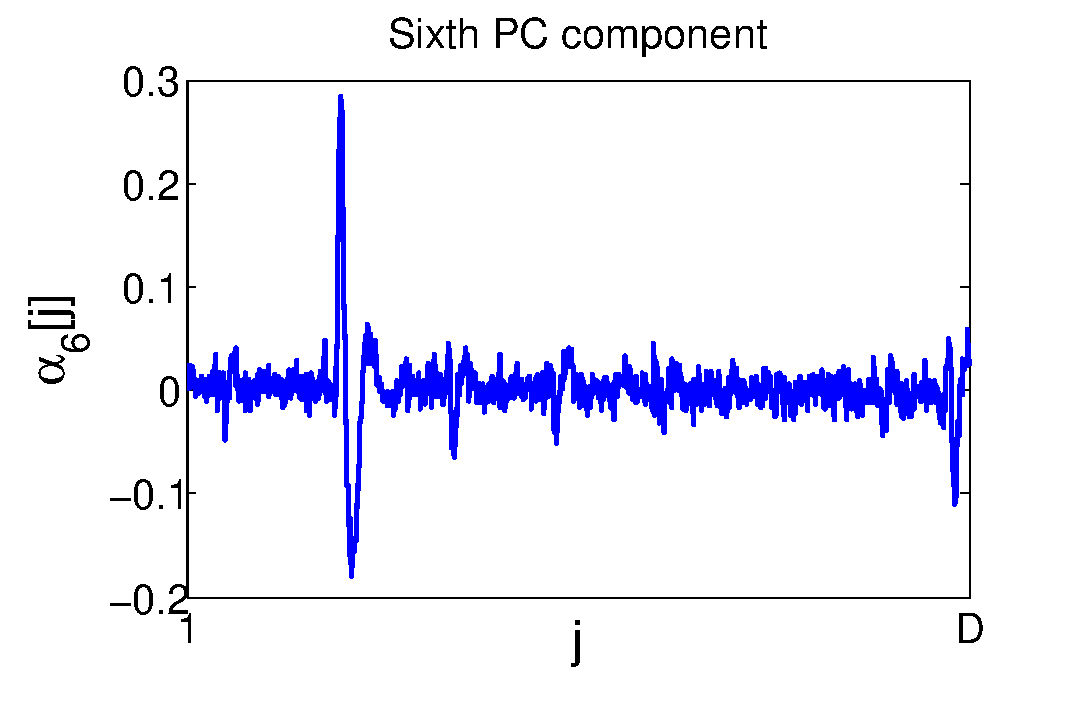
\includegraphics[width=.25\textwidth]{figures/DPAcontestPC6_new.pdf} 
%\vspace{-10pt}
%\caption{First and sixth PCs in DPA contest v4  \cite{DPAcontest} trace set}\label{fig:DPAcontest}
%\end{figure}
%}
%\only<2>{
%\vspace{40pt}
%\begin{small}
%\begin{table}
%\begin{tabular}{|c|c|c|c|}
%\hline
%& EGV \cite{choudaryefficient} & IPR \cite{SCAclassProbl}& \uncover<2->{\textbf{ELV} \cite{Cagli2016}} \\
%\hline
%eigenvalue $\lambda_i$ &
\includegraphics[scale=0.01]{figures/yes.png}  & 
\includegraphics[scale=0.01]{figures/no.png} &\uncover<2->{
\includegraphics[scale=0.015]{figures/yes.png}}\\
%\hline
%form of $\AAlpha_i$ &
\includegraphics[scale=0.01]{figures/no.png}  & 
\includegraphics[scale=0.01]{figures/yes.png}&\uncover<2->{
\includegraphics[scale=0.015]{figures/yes.png}} \\
%\hline
%\end{tabular}
%\end{table}
%\end{small}
%
%\includegraphics[scale=0.3]{figures/citazione1.jpg} 
%}
%\uncover<2->{
%\begin{block}{Explained Local Variance}
%$\mathrm{ELV}(\AAlpha_i,j) = \frac{\lambda_i \AAlpha_i[j]^2}{\sum_{k=1}^r\lambda_k} = \mathrm{EGV}(\AAlpha_i) \AAlpha_i[j]^2$  \\
%%($\sum_{j=1}^D \mathrm{ELV}(\AAlpha_i,j) = \EGV{\AAlpha_i}$)
%\end{block}
%}
%\uncover<3->{\begin{block}{Use of the ELV}
%\begin{itemize}
%\item Sort in decreasing order the maximal ELV provided by each component $\{\max_{j=1,\dots,D}\ELV(\AAlpha_i,j)\}_{i}$ and select the $C$ first components.
%\item Select \textbf{couples} $(\AAlpha_i, j)$ in decreasing order wrt to $\ELV(\AAlpha_i, j)$ until $\ELV(\AAlpha_{i_1}, j_1)+ \ELV(\AAlpha_{i_2}, j_2)+\dots +\ELV(\AAlpha_{i_M}, j_M)\geq \beta$
%\end{itemize}
%\end{block}}
%\end{frame}

%\begin{frame} \frametitle{The ELV Selection (2)}
%\vspace*{-0.5cm}
%\uncover<1->{
%\begin{block}{Definition}
%$\mathrm{ELV}(\AAlpha_i,j) = \frac{\lambda_i \AAlpha_i[j]^2}{\sum_{k=1}^r\lambda_k} = \mathrm{EGV}(\AAlpha_i) \AAlpha_i[j]^2$  \\
%\uncover<2->{Observe that $\sum_{j=1}^D \mathrm{ELV}(\AAlpha_i,j) = \EGV{\AAlpha_i}$}
%\end{block}
%}
%\uncover<3->{
%Perform this sum in a cumulative way, sorting the ELV contributions of the time samples in decreasing order, {\em i. e.} $\mathrm{ELV}(\AAlpha_i,j^i_1)\geq \mathrm{ELV}(\AAlpha_i,j^i_2)\geq \dots \geq \mathrm{ELV}(\AAlpha_i,j^i_\traceLength)$
%
%
%\vspace*{-0.4cm}
%\begin{columns}
%\begin{column}{.5\textwidth}
%\vspace*{10pt}
%\begin{figure}
%\includegraphics[width=\textwidth]{figures/PC1_points.pdf} 
%\end{figure}
%\end{column}
%\begin{column}{.5\textwidth}
%\begin{figure}
%
%\begin{tikzpicture}[remember picture,
%    scale=1,
%    % Define styles here
%    every node/.style={transform shape}
%    block/.style={
%        rectangle,
%        draw,
%        text centered,
%        rounded corners
%        },
%    data/.style={
%        trapezium,
%        trapezium left angle=60,
%        trapezium right angle=120,
%        draw
%        },
%    component/.style={
%        circle,
%        draw
%        },
%    output/.style={
%        tape,
%        tape bend top=none,
%        draw
%        },
%    edge/.style={
%        ->,
%        >=stealth,
%        thick
%        }
%    ]
%
%    \node (only1elv) at (0,0)
%    {\includegraphics[width=\textwidth]{figures/cumulativeELV_only1.pdf} };
%    \node [component, thick, xshift=2.1cm, yshift=0.8cm] (cerchio) {};
%    \node[below left=1cm of cerchio](caption){$\mathrm{EGV}(\AAlpha_1)$};
%    \draw[->] (caption) to (cerchio.south west);
%\end{tikzpicture}
%\end{figure}
%\end{column}
%\end{columns}
%
%
%}
%
%\end{frame}



%\begin{frame}
%\frametitle{The ELV Selection (2)}
%\begin{columns}
%\begin{column}{0.5\textwidth}
%\uncover<1->{
%\only<1>{
%\vspace*{-0.4cm}
%\begin{center}
%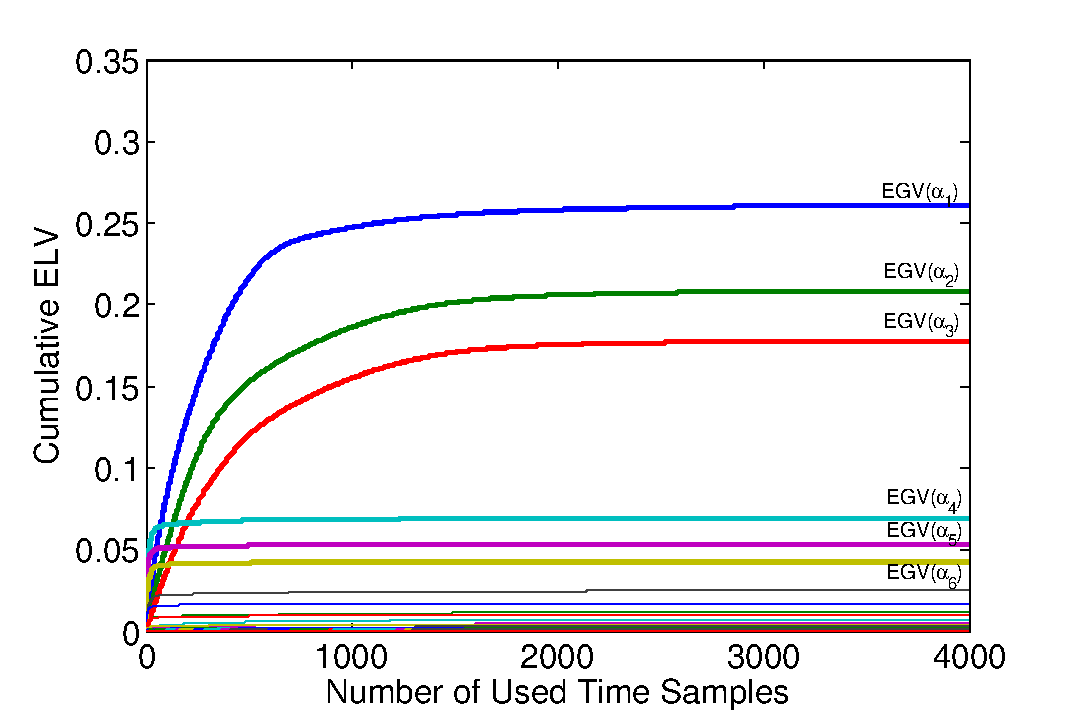
\includegraphics[width = \textwidth]{figures/cumulativeELV.pdf}
%\end{center}
%}
%\only<2>{
%\vspace*{-0.4cm}
%\begin{center}
%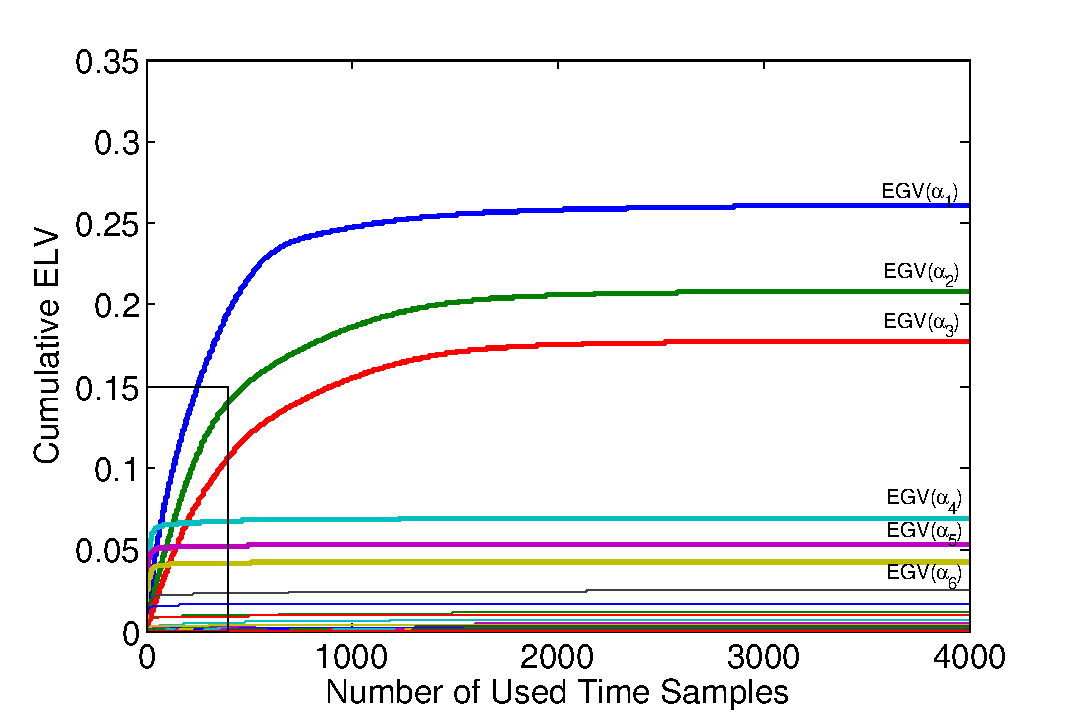
\includegraphics[width = \textwidth]{figures/cumulativeELVallRectangle.pdf} 
%\end{center}
%}
%
%\only<3->{
%\vspace*{-0.4cm}
%\begin{center}
%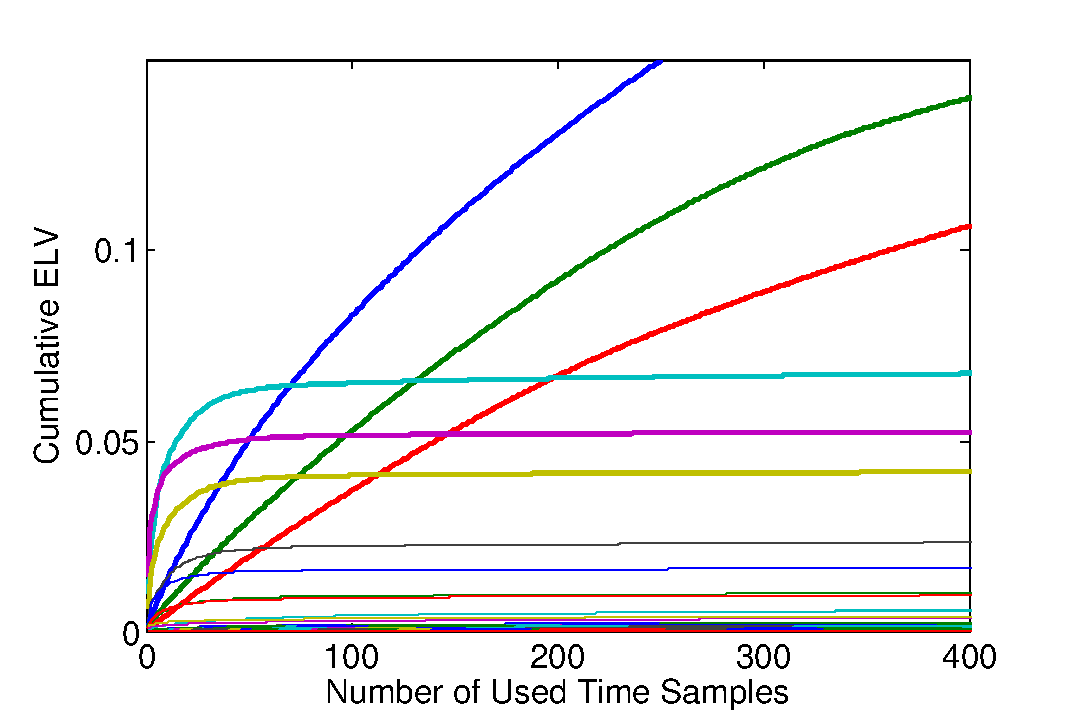
\includegraphics[width = \textwidth]{figures/cumulativeELVzoomed.pdf}
%\end{center}
%}
%}
%\uncover<4->{
%\only<1-4>{
%
%\begin{block}{To select $C$ components\hspace{\textwidth}\textcolor{white}{ }}
%Sort in decreasing order the maximal ELV provided by each component $\{\max_{j=1,\dots,D}\ELV(\AAlpha_i,j)\}_{i}$ and select the $C$ first components.
%\end{block}
%}
%\only<5>{
%
%\begin{block}{Fixing a cumulative explained variance threshold $\beta$}
%Select \textbf{couples} $(\AAlpha_i, j)$ in decreasing order wrt to $\ELV(\AAlpha_i, j)$ until $\ELV(\AAlpha_{i_1}, j_1)+ \ELV(\AAlpha_{i_2}, j_2)+\dots +\ELV(\AAlpha_{i_M}, j_M)\geq \beta$.\\
%%\uncover<5>{{\em Components denoising}}
%\end{block}
%}
%}
%
%\end{column}
%
%\begin{column}{0.5\textwidth}
%\only<1-3>{
%\begin{figure}
%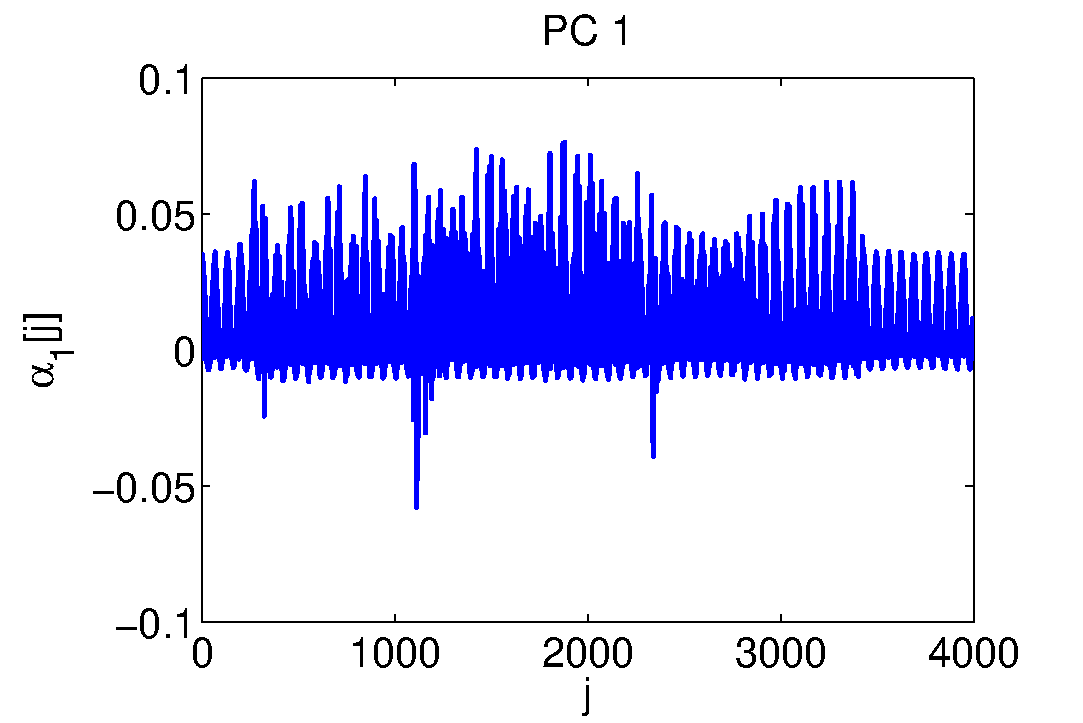
\includegraphics[width=0.5\textwidth]{figures/PC1.pdf} 
%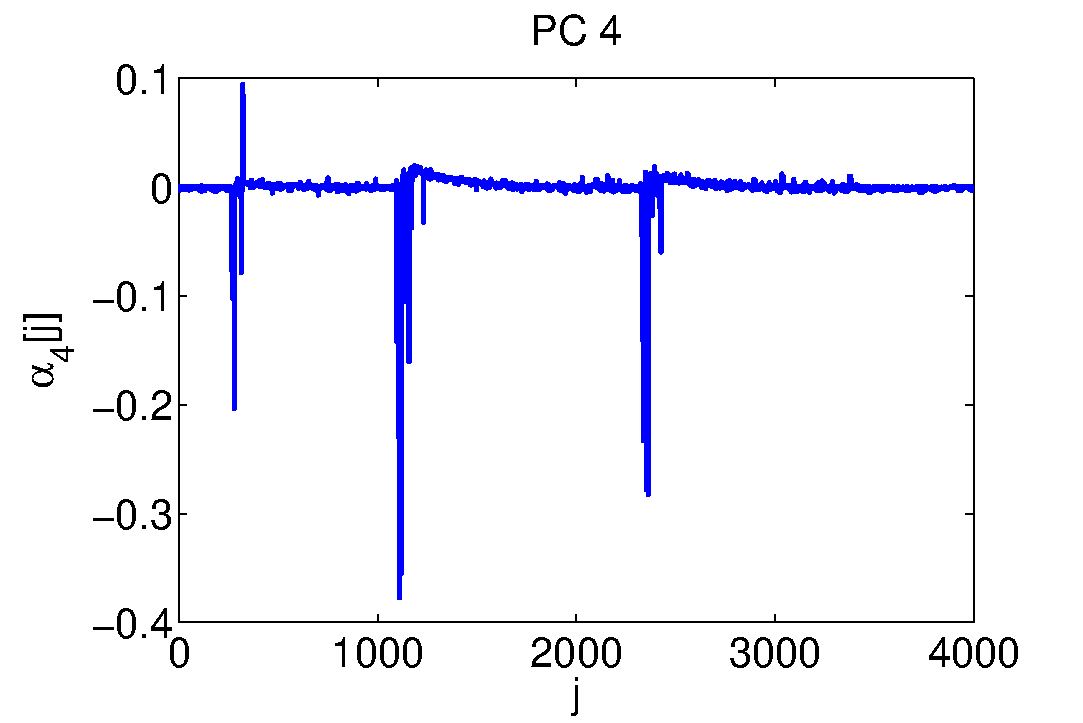
\includegraphics[width=0.5\textwidth]{figures/PC4.pdf} \\
%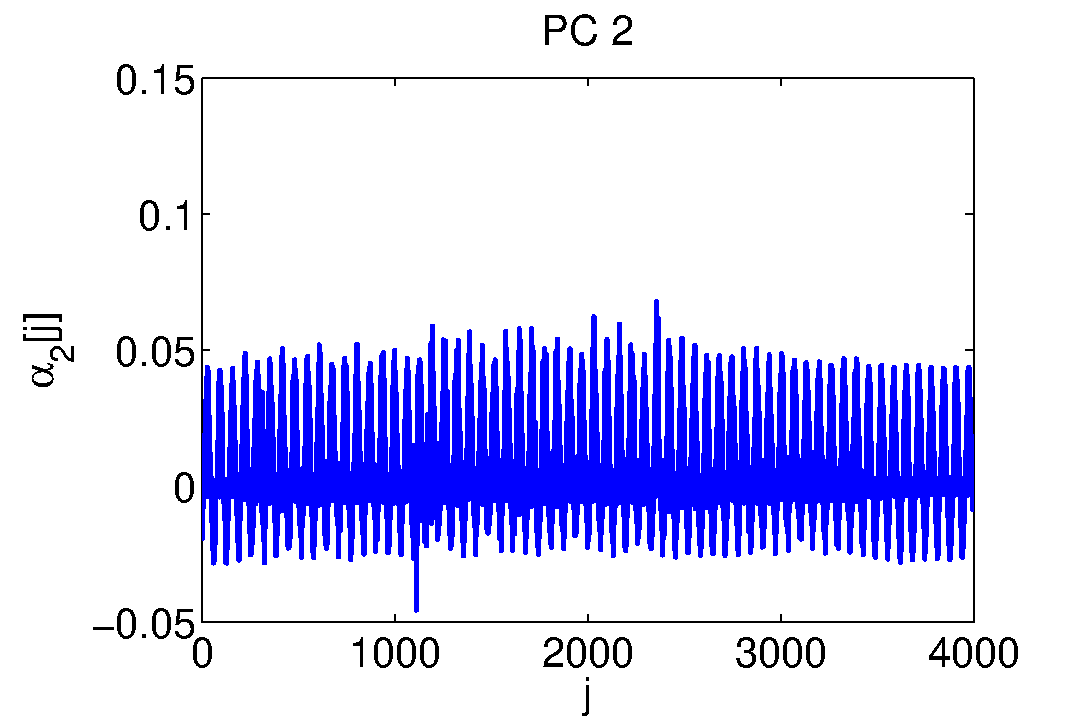
\includegraphics[width=0.5\textwidth]{figures/PC2.pdf} 
%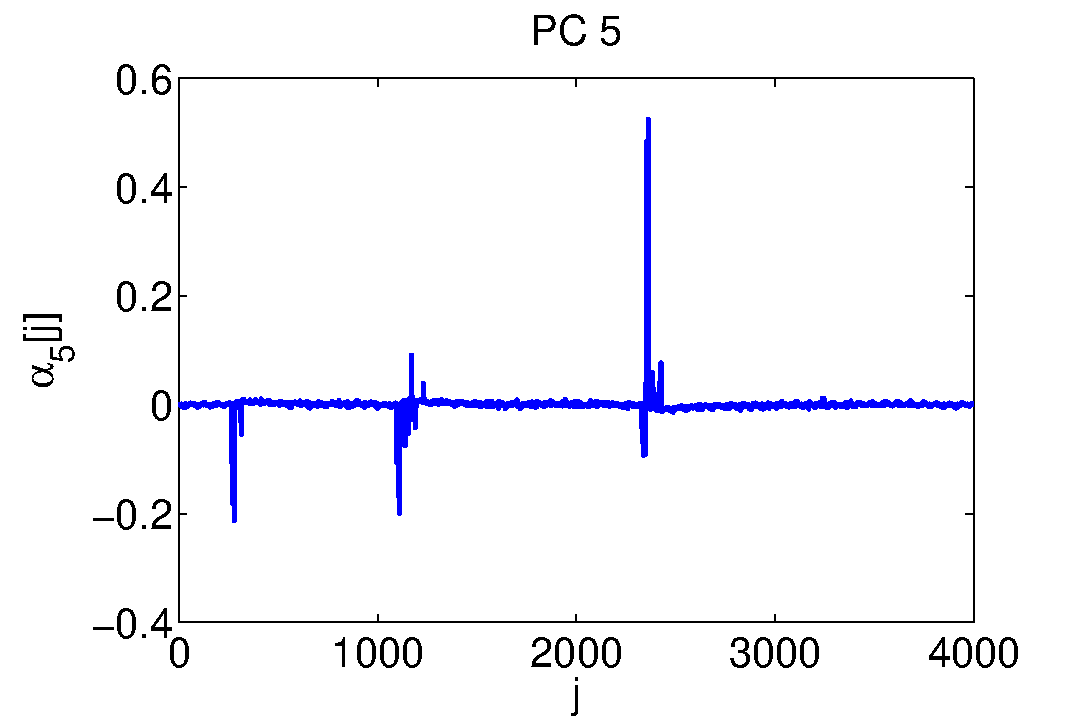
\includegraphics[width=0.5\textwidth]{figures/PC5.pdf} \\
%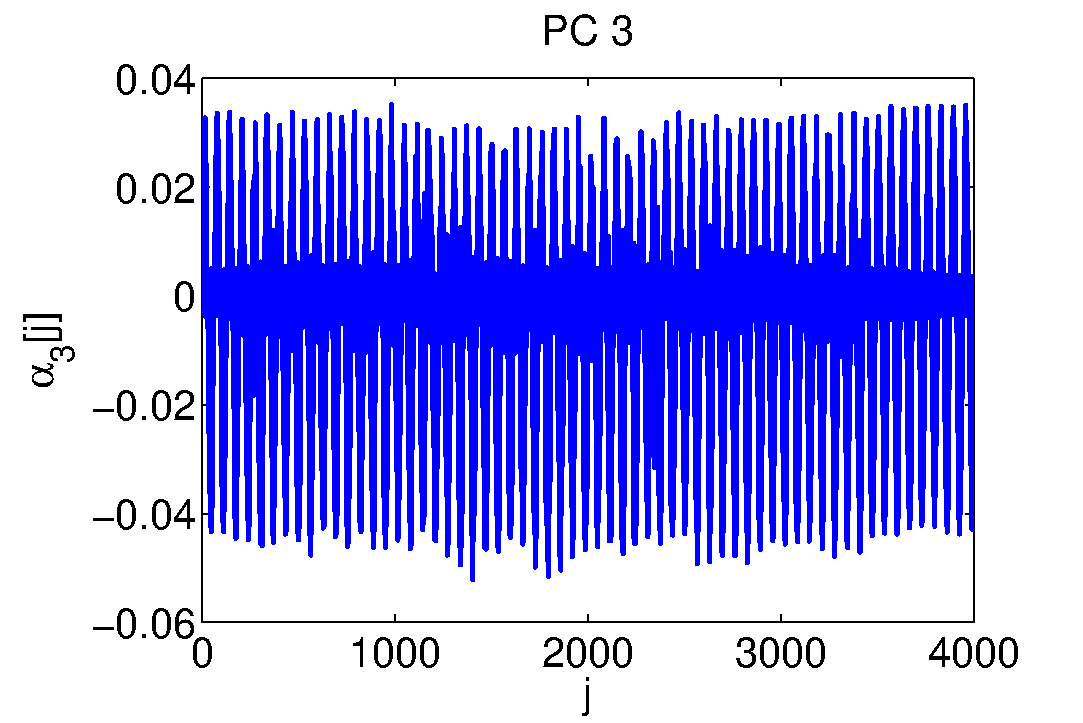
\includegraphics[width=0.5\textwidth]{figures/PC3.pdf} 
%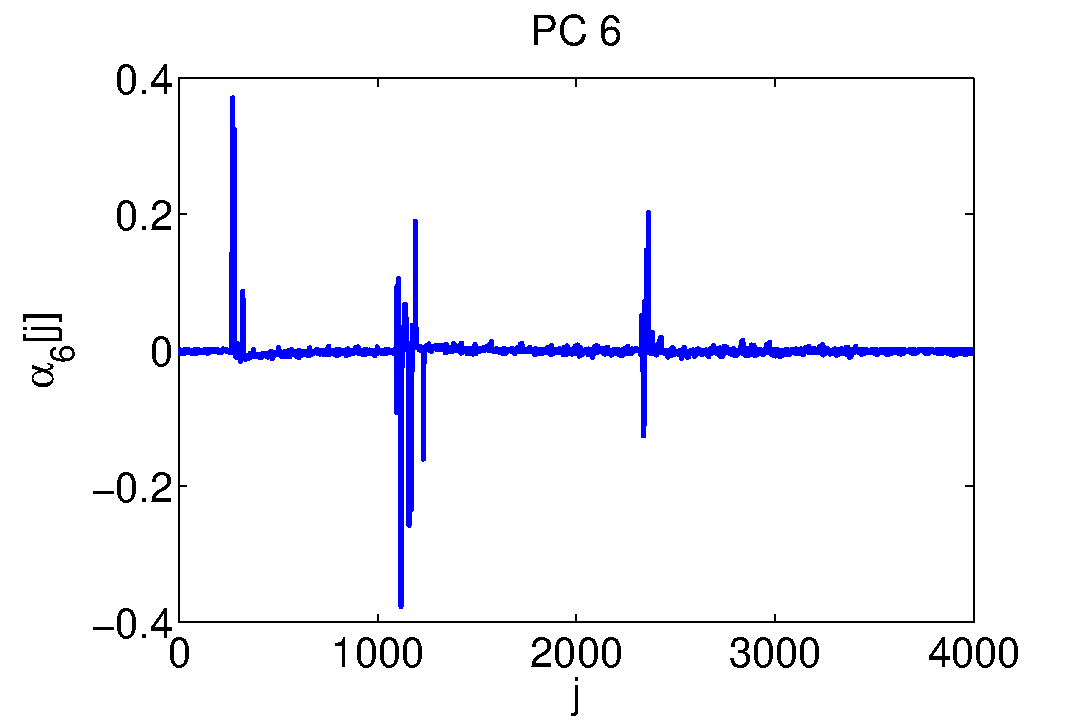
\includegraphics[width=0.5\textwidth]{figures/PC6.pdf} 
%\caption{\begin{footnotesize}
%The first 6 PCs: 
%$\lambda_1 \approx 3.8 ,\lambda_2 \approx 3.1 , \lambda_3 \approx2.6 ,\lambda_4 \approx 1.0 ,\lambda_5 \approx 0.8 ,\lambda_6 \approx 0.6 $
%\end{footnotesize}}
%
%\end{figure}
%}


%\only<4-5>{
%\begin{figure}
%\onslide<5->{\includegraphics[width=0.5\textwidth]{figures/PC5_denoised.pdf}}\only<4>{\includegraphics[width=0.5\textwidth]{figures/PC5_cerchio.pdf}}\only<5>{\includegraphics[width=0.5\textwidth]{figures/PC5_cerchio_transp.pdf}} \\
%\onslide<5->{\includegraphics[width=0.5\textwidth]{figures/PC4_denoised.pdf}}\only<4>{\includegraphics[width=0.5\textwidth]{figures/PC4_cerchio.pdf}}\only<5>{\includegraphics[width=0.5\textwidth]{figures/PC4_cerchio_transp.pdf}} \\
%\onslide<5->{\includegraphics[width=0.5\textwidth]{figures/PC6_denoised.pdf}}\only<4>{\includegraphics[width=0.5\textwidth]{figures/PC6_cerchio.pdf}}\only<5>{\includegraphics[width=0.5\textwidth]{figures/PC6_cerchio_transp.pdf}} 
%\only<4>{\caption{The 3 components chosen by ELV selection method - $C$ fixed}}
%\only<5>{\caption{Components and time samples chosen by ELV selection method - $\beta$ fixed}}
%\end{figure}
%}


%\only<5>{
%\includegraphics[width=0.31\textwidth]{figures/PC5_cerchio_transp.pdf} 
%\includegraphics[width=0.31\textwidth]{figures/PC4_cerchio_transp.pdf} 
%\includegraphics[width=0.31\textwidth]{figures/PC6_cerchio_transp.pdf} \\
%}
%\uncover<5>{
%
%
%
%\only<3-4>{\caption{Selected components for $C = 3$; \hspace{\textwidth} $\ELV(\AAlpha_5, 2362)\approx 0.41$, $\ELV(\AAlpha_4, 1110)\approx 0.38$, $\ELV(\AAlpha_6, 1118)\approx 0.24$}}
%\only<5>{\caption{Selected and denoised components for $\beta = 0.08$\hspace{\textwidth}\textcolor{white}{$\ELV(\AAlpha_5, 2362)\approx 0.41$, $\ELV(\AAlpha_4, 1110)\approx 0.38$, $\ELV(\AAlpha_6, 1118)\approx 0.24$}}}
%
%\end{column}
%
%\end{columns}
%
%
%\end{frame}

%\subsection{Linear Discriminant Analysis}
%
%
%\subsubsection{The Small Sample Size (SSS) Problem}
%
%\begin{frame} \frametitle{The Small Sample Size (SSS) Problem}
%\begin{block}{The SSS Problem}
%$\SW$ has to be invertible \\
%
%
%Necessary condition: the total number of acquisition used to construct $\SW$ must be higher than $D$
%\end{block}
%
%
%\begin{block}{A Glance to the Pattern Recognition State of the Art}
%Four methods: 
%\begin{itemize}
%\item \cite{eigenfaces}: Fisherface
%\item \cite{Chen2000} : $\SW$ Null Space
%\item \cite{Yu01adirect} : Direct LDA
%\item \cite{huang} : $\ST$ Spanned Space 
%\end{itemize}
%\end{block}
%\end{frame}
%

%\subsection{Experimental Results}
%
%
%
%
%
%\begin{frame}
%\vspace*{-2pt}
%\frametitle{Experimental results (minimizing $N_a$)}
%\vspace{-10pt}
%\begin{figure}[t]
%\includegraphics[width=0.4\textwidth]{figures/Criterion1.pdf}
%\includegraphics[width=0.4\textwidth]{figures/Criterion1Good.pdf}
%\caption{Guessing Entropy as function of the number of attack traces.}
%\end{figure}
%\vspace{-10pt}
%\begin{block}{Observations}
%\begin{itemize}
%\item LDA optimal (but more expensive)
%\item PCA close to LDA if equipped with ELV (and less expensive)
%\end{itemize}
%\end{block}
%
%\end{frame}
%
%\begin{frame}
%\vspace*{-2pt}
%\frametitle{Experimental results (minimizing $N_p$)}
%
%\vspace{-10pt}
%\begin{figure}
%\includegraphics[width=0.4\textwidth]{figures/SSS.pdf}
%\includegraphics[width=0.4\textwidth]{figures/Criterion2notSSS.pdf}
%\caption{Guessing Entropy as function of the number of profiling traces.}
%\end{figure}
%
%\begin{block}{Observations}
%\begin{itemize}
%\item if LDA unavailable: PCA$+$ELV best alternative
%\item if LDA available: its efficiency is affected by the lack of profiling traces, PCA $+$ ELV keeps better
%\end{itemize}
%\end{block}
%
%\end{frame}
%\section{Kernel Discriminant Analysis against Masking}


\subsection{Linear Discriminant Analysis}

%\begin{frame}
%\frametitle{Contents}
%\begin{itemize}
%\item \important{Introduction to LDA: as a classifier, and as a feature extractor}
%\item Introduction to masking countermeasure and Kernel Discriminant Analysis as a feature extractor
%\item Motivations to apply deep learning techniques
%\item Convolutional Neural Networks and Data Augmentation to attack jitter-based countermeasure
%\end{itemize}
%\end{frame}



\begin{frame}
\frametitle{Model-based SNR and Fisher's Criterion}
\vspace*{-12pt}
\begin{block}{Signal-to-Noise Ratio (SNR)}
\begin{itemize}
\item Independent Noise Assumption: $\vaLeakVec = \varphi(\sensRandVar)+\vec{B}$

\item $\mmmXclass= \esperEst[\given{\vaLeakVec}{\sensRandVar = \sensVarGenValue}] = \frac{1}{\nbTracesPerClass}\sum_{i\colon \sensVar_i=\sensVarGenValue} \vLeakVec_i $ sample mean per class ($\approx \varphi(\sensRandVar)$)
\item $\varXclass = \varEst(\given{\vaLeakVec}{\sensRandVar = \sensVarGenValue}) = \frac{1}{\nbTracesPerClass-1}\sum_{i\colon \sensVar_i=\sensVarGenValue} (\vLeakVec_i - \mmmXclass)^2 $ sample variance per class ($\approx \mathrm{var}(\vec{B})$) 
\item \begin{equation*}\mathrm{SNR}(t) = \frac{\varEst(\mmmXclass[Z](t))}{\esperEst[\varXclass[Z](t)]} \qquad \textcolor{grey}{\frac{\text{\emph{variance inter-class}}}{\text{\emph{variance intra-class}}}} \end{equation*}
\end{itemize}
\end{block}

\begin{block}{Fisher's Criterion for Linear Dimensionality Reduction}

\begin{itemize}
\item $\SB = \sum_{\sensVarGenValue\in\sensVarSet}\nbTracesPerClass(\mmmXclass-\mmmX)(\mmmXclass-\mmmX)^\intercal $ (inter-class scatter matrix)
\item $\SW = \sum_{\sensVarGenValue\in\sensVarSet}\sum_{i=1\colon \sensVar_i=\sensVarGenValue}(\vLeakVec_i-\mmmXclass)(\vLeakVec_i-\mmmXclass)^\intercal$ (intra-class scatter matrix)
\item Fisher's criterion
 \begin{equation}\label{eq:LDA}
\hat{ \AAlpha}=\mathrm{argmax}_{\AAlpha} \frac{\AAlpha^\intercal \SB \AAlpha}{\AAlpha^\intercal \SW \AAlpha} \mbox{ ,}
 \end{equation}
 $\extract(\vLeakVec) = A\vLeakVec $ where $A=[\AAlpha_1, \dots, \AAlpha_{|\sensVarSet|-1}]$ eigenvectors of $\SW^{-1}\SB$
\end{itemize}

\end{block}
\end{frame}

\begin{frame}
\frametitle{LDA: an optimal binary linear classifier}
\begin{columns}
\begin{column}{.5\linewidth}
\includegraphics[width=\textwidth]{figures/dataNoProjection.pdf} 
\end{column}
\begin{column}{.6\linewidth}
\begin{itemize}
\item Classify data $\vLeakVec$ into 2 classes $\sensVarSet = \{\sensVarValue{1}, \sensVarValue{2}\}$
\pause
\item Generative model: $\pdf_{\given{\vaLeakVec}{\sensRandVar = \sensVarValue{j}}}(\vLeakVec)$, $\pdf_{\sensRandVar}(\sensVarValue{j})$ and $\pdf_{\vaLeakVec}(\vLeakVec)$
\pause
\item Posterior probabilities (via Bayes' theorem), then classify through the \emph{log-likelihood ratio}: $a = \log\left[\frac{\prob(\given{\sensVarValue{1}}{\vLeakVec})}{\prob(\given{\sensVarValue{2}}{\vLeakVec})}\right]]$ (boundary surface $a=0$)
\end{itemize}
\end{column}
\end{columns}
\pause
\begin{itemize}
\item Two assumptions about class-conditional densities: 
\begin{itemize}
\item Gaussian distributions with parameters $\mu_j, \Sigma_j$
\item Homoscedasticity: $\Sigma_j=\Sigma$ for all $j$
\end{itemize}
\pause
\item $\Rightarrow a = \vec{w}^\intercal \vLeakVec + w_0$ (linear decision boundary, $\vec{w}$ and $w_0$ functions of $\Sigma, \mu_j$)
\end{itemize}
\pause
\begin{block}{Generalised linear discriminative model}
\begin{equation}\label{eq:binary_linear_classifier}
\prob(\given{\sensVarValue{1}}{\vLeakVec}) = \sigma(\www^\intercal \vLeakVec + w_0)\mbox{ ,where }  \sigma(a)= \frac{1}{1+e^{-a}} \text{\emph{logistic sigmoid}}
\end{equation}
\end{block}
\end{frame}

\begin{frame}
\frametitle{LDA and Fisher's Discriminant}
\begin{columns}
\begin{column}{.5\linewidth}
\only<1>{\includegraphics[width=\textwidth]{figures/LDA_boundary.pdf}}
\only<2->{\includegraphics[width=\textwidth]{figures/LDAprojection.pdf} }
\end{column}
\begin{column}{.6\linewidth}
\begin{itemize}
\item LDA: linear decision boundary $a = \vec{w}^\intercal \vLeakVec + w_0$
\pause
\item Equivalently, project data onto $\vec{w}^\intercal \vLeakVec$ (orthogonally to the decision boudary), than classify by a real threshold (optimally $w_0$). \\
\end{itemize}
\end{column}
\end{columns}
\pause
\begin{itemize}
\item Two assumptions about class-conditional densities: 
\begin{itemize}
\item Gaussian distributions with parameters $\mu_j, \Sigma_j$
\item Homoscedasticity: $\Sigma_j=\Sigma$ for all $j$
\end{itemize}
\end{itemize}

\begin{block}{Fact, abuse and preference for the dimensionality reduction formulation}
\begin{itemize}
\item When LDA assumptions are met, the solution $\AAlpha_1$ of the Fisher's criterion is orthogonal to $\vec{w}$. 
\item assumption not required
\item naturally multi-class
\end{itemize}
\end{block}

\end{frame}

\begin{frame}
\frametitle{Linear separability}

\only<1>{\includegraphics[width=0.5\textwidth]{figures/LDA_non_linearly.pdf}\\ }
LDA: linear decision boundary $a = \vec{w}^\intercal \vLeakVec + w_0$ ($\vec{w} = \Sigma^{-1}(\mu_1-\mu_2)$)
%
\begin{block}{}
\begin{huge}
\centering What if $\mu_1 = \mu_2$? 
\end{huge}
\end{block}
\only<2>{\includegraphics[width=.4\textwidth]{figures/D2.png}\\}
\only<3>{\includegraphics[width=.4\textwidth]{figures/D2.png}\includegraphics[width=.4\textwidth]{figures/D2_useless1.png}\\}
\only<4>{\includegraphics[width=.4\textwidth]{figures/D2.png}\includegraphics[width=.4\textwidth]{figures/D2_useless2.png}\\}
\only<5>{\includegraphics[width=.4\textwidth]{figures/D2.png}\includegraphics[width=.4\textwidth]{figures/D2_useless3.png}\\}
\only<6>{\includegraphics[width=.4\textwidth]{figures/D2.png}\includegraphics[width=.4\textwidth]{figures/D2_useless4.png}\\}
\uncover<2->{$f(z) = \esper[\vaLeakVec\lvert Z=z]$ is constant\\}
\uncover<3->{$\esper[A\vaLeakVec\lvert Z=z]$ is constant as well $\Rightarrow$ Projecting extractors can't help! }
\end{frame}


\begin{frame}
\frametitle{Dimensionality reduction in presence of masking}
\begin{block}{$(d-1)$th-order Sharing (or Masking)} 
Split each sensitive $Z$ into shares  $Z = M_1 \star \dots \star M_d$ \\
with \only<1-2>{\textcolor{black}{$M_1, \dots , M_{d-1}$}}\only<3->{\textcolor{red}{$M_1, \dots , M_{d-1}$}} random shares (or masks) \only<3->{\textcolor{red}{UNKNOWN}} \\ and $M_d = Z \star M_1^{-1}\star \dots \star M_{d-1}^{-1}$ \\
Software implementations: shares are handled at different time samples $$t_1,\dots, t_d \qquad \only<1-2>{\mbox{\textcolor{white}{UNKNOWN}}} \only<3->{\mbox{\textcolor{red}{UNKNOWN}}} $$\\
$\Rightarrow$ each time sample is independent from $Z$.\\
\end{block}
\uncover<2->{
\begin{columns}
\begin{column}{.5\textwidth}
\includegraphics[width=\textwidth]{figures/D2.pdf}
\end{column}
\begin{column}{.5\textwidth}
\begin{block}{}
Toy example: 2 time samples, 1-bit data
\begin{itemize}
\item[$t_1$:] $M + n$, $n\sim \mathcal{N}(0,0.1)$ 
\item[$t_2$:] $M\oplus Z + n$ (Boolean masking)
\end{itemize}
\end{block}
\end{column}
\end{columns}
}
\end{frame}



\begin{frame}
\frametitle{In high-dimensional traces}
$f(z) = \esper[\vaLeakVec\lvert Z=z]$ is constant $\Rightarrow$ SNR, SOD, t-statistic are null!
\includegraphics[width = 0.9\textwidth]{figures/SNR_2order_new.png} \\
\pause
$\esper[A\vaLeakVec\lvert Z=z]$ is constant as well 

\begin{block}{Higher-Order Side-Channel Attacks}
Exploit $f(z) = \esper\left[\vaLeakVec[t_1]\vaLeakVec[t_2]\dots\vaLeakVec[t_d]\lvert Z=z\right]$ non-constant.
 \end{block}

\begin{block}{Necessary condition}
\cite{carlet2014achieving} The statistic extracted from measurements must contain  $$\vaLeakVec[t_1]\vaLeakVec[t_2]\dots\vaLeakVec[t_d]$$
\end{block} 
\end{frame}

\begin{frame}
\frametitle{PoIs Research}
How to detect the $d$-tuple $t_1,\dots, t_d$? 
\begin{block}{A lacking literature}
\begin{itemize}
\item many HO attacks papers assume the knowledge of $t_1,\dots, t_d$
\item PoI research exploiting the random shares knowledge (back to unprotected case using $M_1,\dots , M_d$ instead of $Z$)
\item naive strategy: infer over all possible $d$-tuples 
\item Hand selection via educated guess \cite{Oswald2006}
\end{itemize}
\end{block}

\begin{block}{Generalizing extractors for higher-order context}
\begin{itemize}
\item Selecting extractors $\longrightarrow$ Projection Pursuits \cite{PP}
\item Projecting extractors $\longrightarrow$ Kernel Discriminant Analysis [CARDIS '16]
\end{itemize}
\end{block}
\end{frame}

\subsection{Kernel Discriminant Analysis}

\begin{frame}
[fragile]
\frametitle{KDA: the purpose}

\begin{block}{Problem}
Useful statistics lie in a high-dimensional \emph{feature} space: 
$$\featureSpace = \mathbb{R}^{{D+d-1}\choose{d}}$$
(all $d$th-degree monomials in the trace coordinates)
\end{block}

\begin{figure}
\centering
{
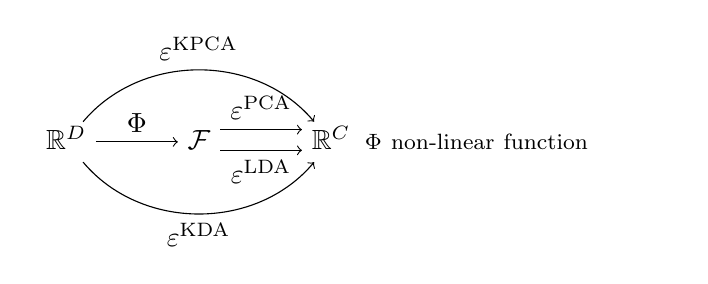
\begin{tikzpicture}
\matrix (m) [matrix of math nodes, row sep=3em,
column sep=3em, text height=1.5ex, text depth=0.25ex]
{ \mathbb{R}^\traceLength & \featureSpace & \mathbb{R}^\newTraceLength \\};
\path[->]
(m-1-1) edge node[above] {$\Phi$} (m-1-2);
         %edge [bend left=30] (m-2-2)
         %edge [bend right=15] (m-2-2);
\path[->]
($(m-1-2.north east)-(0,0.1)$) edge node[above] {$\extract^{\mathrm{PCA}}$} ($(m-1-3.north west)-(0,0.1)$);
\path[->]
($(m-1-2.south east)+(0,0.15)$) edge node[below] {$\extract^{\mathrm{LDA}}$} ($(m-1-3.south west)+(0,0.15)$);

\path[->]
(m-1-1) edge [bend left=50] node[above] {$\extract^{\mathrm{KPCA}}$} (m-1-3)
(m-1-1) edge [bend right=50] node[below] {$\extract^{\mathrm{KDA}}$} (m-1-3);

\node[text width=4cm] at (4,0) {\begin{footnotesize}
$\Phi$ non-linear function
\end{footnotesize}};
\end{tikzpicture} 
}


\end{figure}

\begin{block}{What KDA provides}
KDA allows performing LDA in $\featureSpace$, remaining in $\mathbb{R}^{D}$.
\end{block}

\end{frame}



\begin{frame}
%[fragile]
\frametitle{KDA: an intuition}
%\vspace{-30pt}
%\begin{figure}
%\centering
%{
%\begin{tikzpicture}
%\matrix (m) [matrix of math nodes, row sep=3em,
%column sep=3em, text height=1.5ex, text depth=0.25ex]
%{ \mathbb{R}^\traceLength & \featureSpace & \mathbb{R}^\newTraceLength \\};
%\path[->]
%(m-1-1) edge node[above] {$\Phi$} (m-1-2);
%         %edge [bend left=30] (m-2-2)
%         %edge [bend right=15] (m-2-2);
%\path[->]
%($(m-1-2.north east)-(0,0.1)$) edge node[above] {$\extract^{\mathrm{PCA}}$} ($(m-1-3.north west)-(0,0.1)$);
%\path[->]
%($(m-1-2.south east)+(0,0.15)$) edge node[below] {$\extract^{\mathrm{LDA}}$} ($(m-1-3.south west)+(0,0.15)$);
%
%\path[->]
%(m-1-1) edge [bend left=50] node[above] {$\extract^{\mathrm{KPCA}}$} (m-1-3)
%(m-1-1) edge [bend right=50] node[below] {$\extract^{\mathrm{KDA}}$} (m-1-3);
%
%\node[text width=4cm] at (4,0) {\begin{footnotesize}
%$\Phi$ non-linear function: all $d$th-degree monomials of time samples
%\end{footnotesize}};
%\end{tikzpicture} 
%}
%
%
%\end{figure}
\vspace{-15pt}
\begin{block}{}
Toy example: 2 time samples, 1-bit data
\begin{itemize}
\item[$t_1$:] $M + n$, $n\sim \mathcal{N}(0,0.1)$ 
\item[$t_2$:] $M\oplus Z + n$ (Boolean masking)
\end{itemize}
\end{block}

\begin{columns}
\begin{column}{.5\textwidth}
\uncover<1->{
\only<1-3>{
\begin{figure}
\includegraphics[width=\textwidth]{figures/D2.pdf}
\end{figure}}

\only<4>{
\begin{figure}
\includegraphics[width=\textwidth]{figures/D2_proj.pdf}
\end{figure}
\centering
\textcolor{violet}{\Large{KDA} \\ \large{remains in $\mathbb{R}^D$}}
}
\only<5->{
\begin{figure}
\includegraphics[width=\textwidth]{figures/new_example_KDA.pdf} 
\end{figure}}
}

\end{column}

\begin{column}{.5\textwidth}
\uncover<2->{
\only<1-2>{
\begin{figure}
\includegraphics[width=\textwidth]{figures/D3.pdf} 
\end{figure}
\centering
\textcolor{violet}{\Large{ $\Phi\colon \mathbb{R}^D \rightarrow \mathbb{R}^{{D+d-1}\choose{d}}$  \\ $\Phi(t_1,t2) = (t_1^2, t_2^2, kt_1t_2)$ }}
}
\only<3>{
\begin{figure}
\includegraphics[width=\textwidth]{figures/D3_proj.pdf} 
\end{figure}
\centering
\textcolor{violet}{\Large{$\Phi \longrightarrow$ LDA}}
}
\only<4>{
\begin{figure}
\includegraphics[width=\textwidth]{figures/D3_proj.jpg} 
\end{figure}
}}

\only<5->{
\begin{block}{KDA procedure}
\begin{itemize}
\item Training $\rightarrow \textcolor{violet}{\boldsymbol{\nu}_\ell}$ , $C$ vectors of coefficients ($\ell = 1,\dots , C$)
\item<6-> \emph{Compare} the new trace with all training traces $K(\textcolor{red}{\sss[z_i]{i}}, \textcolor{green}{\sss[]{}})$, $K(\textcolor{blue}{\sss[z_i]{i}}, \textcolor{green}{\sss[]{}})$
\item<7-> \emph{KDA projection} \begin{equation}\label{eq:projection}
\extract^{\mathrm{KDA}}_{\ell}(\vec{x}) = \sum_{i=1}^{\NPoI}\textcolor{violet}{\boldsymbol{\nu}_\ell[i]}K(\sss[z_i]{i}, \textcolor{green}{\sss[]{}}) \mbox{ .}
\end{equation} 
\end{itemize}

\end{block}
}

\end{column}
\end{columns}
%\uncover<5>{
%\begin{block}{Apply KDA extractor}
%\begin{equation}\label{eq:projection}
%\extract^{\mathrm{KDA}}_{\ell}(\vec{x}) = \sum_{i=1}^{\NPoI}\boldsymbol{\nu}_\ell[i]K(\textcolor{red}{\sss[z_i]{i}}, \textcolor{green}{\sss[]{}}) \mbox{ .}
%\end{equation} 
%
%
%\end{block}
%}
\end{frame}


\begin{frame}
\frametitle{Kernel Function}

\begin{block}{Kernel Function}
$K\colon\mathbb{R}^D\times \mathbb{R}^D \rightarrow \mathbb{R} \nonumber$
\begin{equation}\label{eq:kernelProperty}
K(\sss[]{i},\sss[]{j}) = \Phi(\sss[]{i})\cdot \Phi(\sss[]{j})
\end{equation}
\end{block}

\begin{block}{Polynomial Kernel Function}
$K(\sss[]{i},\sss[]{j}) = (\sss[]{i} \cdot \sss[]{j})^d \qquad \leftrightarrow \qquad\Phi:\mathbb{R}^D \rightarrow \mathcal{F}\subset \mathbb{R}^{{D+d-1}\choose{d}} $ all $d$th-degree monomials


\end{block}
\uncover<2->{
\begin{block}{Example: $2$nd Degree Polynomial Kernel Function}
Toy example: $D=2 \longrightarrow \sss[]{i} = [a,b]$ , $\sss[]{j} = [c,d]$
\begin{equation*}
K(\sss[]{i},\sss[]{j}) = (ac + bd)^2 = a^2c^2 + 2abcd + b^2d^2
\end{equation*}
\only<2>{
\textcolor{white}{$K \longleftrightarrow$ $\Phi\colon \Bbb{R}^2\rightarrow\Bbb{R}^3$
\begin{equation*}
\Phi(u,v) =  [u^2, \sqrt{2}uv, v^2]
\end{equation*}}
}
\uncover<3->{
$K \longleftrightarrow$ $\Phi\colon \Bbb{R}^2\rightarrow\Bbb{R}^3$
%\begin{align}
%&\Phi \colon \mathbb{R}^2 \rightarrow \mathbb{R}^3\\
%&\Phi \colon [a,b]\mapsto [a^2, \sqrt{2}ab, b^2]\\
%&\Phi \colon [c,d]\mapsto [c^2, \sqrt{2}cd, d^2].
%\end{align}
\vspace{-5pt}
\only<3>{
\begin{equation*}
\Phi(u,v) =  [u^2, \sqrt{2}uv, v^2]
\end{equation*}}
\only<4>{
\begin{equation*}
\Phi(a,b) =  \textcolor{magenta}{[a^2, \sqrt{2}ab, b^2]}
\end{equation*}
}
\only<5>{
\begin{equation*}
\Phi(c,d) =  \textcolor{blue}{[c^2, \sqrt{2}cd, d^2]}
\end{equation*}
}
}

\only<3>{
\textcolor{white}{$\Phi(\sss[]{i})\cdot \Phi(\sss[]{j}) = {a^2}{c^2} + {\sqrt{2}ab}{\sqrt{2}cd} + {b^2}{d^2} = K(\sss[]{i},\sss[]{j})$}}

\only<4>{
$\Phi(\sss[]{i})\cdot \Phi(\sss[]{j}) = \textcolor{magenta}{a^2}\textcolor{white}{c^2} + \textcolor{magenta}{\sqrt{2}ab}\textcolor{white}{\sqrt{2}cd} + \textcolor{magenta}{b^2}\textcolor{white}{d^2} = K(\sss[]{i},\sss[]{j})$}

\only<5>{
$\Phi(\sss[]{i})\cdot \Phi(\sss[]{j}) = \textcolor{magenta}{a^2}\textcolor{blue}{c^2} + \textcolor{magenta}{\sqrt{2}ab}\textcolor{blue}{\sqrt{2}cd} + \textcolor{magenta}{b^2}\textcolor{blue}{d^2} = K(\sss[]{i},\sss[]{j})$}

\end{block}
}

\end{frame}



\begin{frame}

\frametitle{KDA - the training}
\begin{center}
\only<1>{
Between-class (inter-class) Scatter Matrix }
\only<2>{
Within-class (inter-class) Scatter Matrix }
\only<3>{
Eigenvector problem}
\only<4>{
New trace projection}

\end{center}

\begin{columns}
\begin{column}{.5\textwidth}
\uncover<3->{Computational Complexity $O(D^3)$}
\begin{block}{LDA}
\begin{small}
\begin{itemize}
\item $\SB = \sum_{\sensVar\in\sensVarSet}\numTraces(\mmmXclass-\mmmX)(\mmmXclass-\mmmX)^\intercal$ 
\uncover<2->{\item $\SW = \sum_{\sensVar\in\sensVarSet}\sum_{i=1}^{\numTraces}(\sss{i}-\mmmXclass)(\sss{i}-\mmmXclass)^\intercal$ }
\uncover<3->{\item $\AAlpha_i$ eigenvectors of $\SW^{-1}\SB$ [$D\times D$]}
\uncover<4->{\item $\extract^{LDA}_{\ell}(\xxx) = \sum_{i=1}^D \AAlpha_{\ell}[i]\xxx[i] $}
\end{itemize}
\end{small}
\end{block}
\end{column}

\begin{column}{.55\textwidth}
\uncover<3->{\only<3-4>{Computational Complexity $O(N^3)$}\only<5>{\textcolor{red}{Computational Complexity $O(N^3)$}}}
\begin{block}{KDA}
\begin{small}
\begin{itemize}

\item $\MMM = \sum_{\sensVar\in\sensVarSet}\numTraces(\MMMclass - \MMMT)(\MMMclass-\MMMT)^\intercal$ \footnotemark

\uncover<2->{\item $\NNN = \sum_{\sensVar\in\sensVarSet}\kernelMatrix_\sensVar(\III - \III_{\numTraces})\kernelMatrix_\sensVar^\intercal$ \only<2-4>{\footnotemark} \only<5>{ \textcolor{red}{$+ \mu\III$}}}

\uncover<3->{\item $\nununu_i$ eigenvectors of $\NNN^{-1}\MMM$ [$N\times N$]}
\uncover<4->{\item \only<4>{$\extract^{\mathrm{KDA}}_{\ell}(\vec{x}) = \sum_{i=1}^{\NPoI}\nununu_\ell[i]K(\sss[z_i]{i}, \sss[]{}) $}\only<5->{$\extract^{\mathrm{KDA}}_{\ell}(\vec{x}) =$ \textcolor{red}{$\sum_{i=1}^{\NPoI}$}$\nununu_\ell[i]$\textcolor{red}{$K(\sss[z_i]{i}, \sss[]{})$} }}
\end{itemize}
\end{small}
\end{block}
\end{column}
\end{columns}
\centering
\vspace{8pt}
\only<5>{\textcolor{red}{$\mu$ regularization parameter} $\qquad$ \textcolor{red}{\emph{Memory-based} machine}}

\footnotetext[1]{$\MMMclass$ and $\MMMT$ are two $N$-sized column vectors whose entries are given by: $\MMMclass[z][j] = \frac{1}{\numTraces}\sum_{i:z_i=z}^{\numTraces}K(\sss[z_j]{j},\sss[z_i]{i}), \qquad
\MMMT[j] = \frac{1}{\NPoI}\sum_{i=1}^{\NPoI}K(\sss[z_j]{j},\sss[z_i]{i}) \mbox{ .}$}

\uncover<2->{\footnotetext[2]{$\III$ is a $\numTraces\times \numTraces$ identity matrix, $\III_{\numTraces}$ is a $\numTraces\times \numTraces$ matrix with all entries equal to $\frac{1}{\numTraces}$ and $\kernelMatrix_{\sensVar}$ is the $\NPoI\times \numTraces$ sub-matrix of $\kernelMatrix = (K(\sss[z_i]{i},\sss[z_j]{j}))_{\substack{i=1,\dots,\numTraces[] \\ j=1,\dots,\numTraces[]}}$ storing only columns indexed by the indices $i$ such that $z_i=z$}}
\end{frame}


\subsection{Experimental Results}


\begin{frame}
\frametitle{Experimental setup}
Target device and acquisitions: 

\begin{itemize}
\item 8-bit AVR microprocessor Atmega328P
\item power-consumption acquired via the ChipWhisperer \cite{o2014chipwhisperer} platform
\item $D = 200$, $4$ clock-cycles are selected
\end{itemize}

Sensitive variable: $Z = \mathrm{Sbox_{AES}}(P\oplus K^{\star})$\\
%Leakage:
%\begin{footnotesize}
%
%\begin{itemize}
%\item[$d=2$] $M_1$, $Z\oplus M_1$
%\item[$d=3$] $M_1$, $M_2$, $Z\oplus M_1\oplus M_2$  
%\item[$d=4$] $M_1$,$M_2$,$M_3$, $Z\oplus M_1\oplus M_2 \oplus M_3$  
%\end{itemize}
%\end{footnotesize}
\begin{figure}
\includegraphics[width=0.8\textwidth]{figures/one_trace.pdf}
\end{figure}
%Attack: 
%\begin{itemize}
%\item \emph{KDA profiling traces} ($\sim 9000$) $\rightarrow \extract^{KDA}\colon \mathbb{R}^{200}\rightarrow \mathbb{R}^2$ separating classes
%\item \emph{TA profiling traces} ($\sim 20000$) $\rightarrow$ Gaussian templates per class
%\item \emph{attack traces} $\rightarrow$ attack via maximum likelihood
%\end{itemize}


\end{frame}

%
%
%\begin{frame}
%[fragile]
%\frametitle{Attack Scenario}
%\begin{block}{KDA training phase}
%Build the KDA extractor $\extract^{KDA}$
%\end{block}
%
%\uncover<2->{
%\begin{block}{Gaussian Template Attack}
%\begin{itemize}
%\item<2-> Preprocess profiling and attack traces
%\item<3-> Compute Gaussian templates
%\item<4-> Attack via maximum likelihood
%\end{itemize}
%\end{block}
%}
%
%\begin{figure}
%\centering
%{
%\begin{tikzpicture}[xscale=0.8,yscale=0.4]
%\uncover<2->{
%\node at (1,4.5) [text width=2cm] {\begin{footnotesize}TA profiling traces\end{footnotesize}};
%\node at (4,4.5)[text width=2cm] {\begin{footnotesize}TA attack traces\end{footnotesize}};
%\draw [->] (1,4) -- (1,3);
%\draw [->] (4,4) --(4,3);
%\node [left] at (1,3.5) {$\mathbb{R}^{200}$};
%\node [right] at (4,3.5) {$\mathbb{R}^{200}$};}
%\draw [blue] (0,2) rectangle(5,3);
%\node at (2.5,2.5) {\begin{large}$\extract^{KDA}$\end{large}};
%\uncover<2->{
%\draw [->] (1,2) -- (1,1);
%\draw [->] (4,2) --(4,1);
%\node [left] at (1,1.5) {$\mathbb{R}^{2}$};
%\node [right] at (4,1.5) {$\mathbb{R}^{2}$};
%\node at (1,0.5)[text width=2cm] {\begin{footnotesize}TA profiling traces\end{footnotesize}};
%\node at (4,0.5)[text width=2cm] {\begin{footnotesize}TA attack traces\end{footnotesize}};}
%\uncover<3->{
%\draw [->] (1,0) -- (1,-2);
%\draw [yellow] (0,-3) rectangle(2,-2);
%\node at (1.5,-2.5)[text width=2cm] {\begin{footnotesize}Templates\end{footnotesize}};}
%\uncover<4>{
%\draw [->] (2,-2.5) -- (3,-2.5);
%\draw [->] (4,0) -- (4,-1.5);
%\draw [red] (4,-2.5) circle(1);
%\node at (4.6,-2.5)[text width=2cm] {\begin{footnotesize}Matching\end{footnotesize}};
%\draw [->] (5,-2.5) -- (6,-2.5);
%\node at (7.5,-2.5)[text width=2cm] {$K^\star$};}
%\end{tikzpicture} 
%}
%
%
%\end{figure}
%
%
%\end{frame}



\begin{frame}
\frametitle{Efficiency/Accuracy trade-off}

KDA training set size fixed ($\sim$ 9000 traces) to control efficiency\\

\begin{block}{Adjust the number of classes to gain in accuracy}
$Z = 0,\dots, 255 $\\
\centering
\begin{tabular}{|c|c|c|}
\hline 
\textbf{Model} & \textbf{number of classes} & \textbf{traces per class} \\
Value & 256 & 35\\
HW & 9 & 1000 \\
HW $<,>,= 4$ & 3 & 3000 \\
HW $\leq,> 4$ & 2 & 4500 \\
\hline
\end{tabular}

\end{block}
\end{frame}







\begin{frame}
\frametitle{Attack of second order}
\vspace{-10pt}
\includegraphics[width=0.5\textwidth]{../Figures/CARDIS2016/2order_classes_TA.pdf} 
\uncover<2->{\includegraphics[width=0.5\textwidth]{../Figures/CARDIS2016/good_coeffs.png} }
\begin{block}{Implicit coefficients}

\begin{equation}
\extract^{\mathrm{KDA}}_{\ell}(\sss[]{}) = \sum_{i=1}^{\NPoI}\nununu_\ell[i]K(\sss[z_i]{i}, \sss[]{})= \sum_{j=1}^\traceLength \sum_{k=1}^\traceLength[ \underbrace{(\sss[]{}[j]\sss[]{}[k])}_{\parbox[c]{2cm}{\centering{multiplied \\ time samples}}}\underbrace{(\sum_{i=1}^{\NPoI}\boldsymbol{\nu}_{\ell}[i] \sss[]{i}[j]\sss[]{i}[k])}_{\mbox{implicit  coefficients}}]
\end{equation}


\end{block}
$d=2 \quad \longrightarrow \quad  {{200+2-1}\choose{2}} = 20.100$ implicit coefficients
\end{frame}

\begin{frame}
\frametitle{Third and Fourth Order}
\begin{figure}
\includegraphics[width=0.5\textwidth]{figures/3order_only_9.pdf}
\includegraphics[width=0.5\textwidth]{figures/4order_only_9.pdf}
\end{figure}


\begin{itemize}
\item $d=3 \quad \longrightarrow \quad {{200+3-1}\choose{3}} = 1.353.400$ implicit coefficients
\item  $d=4 \quad \longrightarrow \quad {{200+4-1}\choose{4}} = 68.685.050$ implicit coefficients
\end{itemize}

Same time of execution of the KDA algorithm!

\end{frame}

%\begin{frame}
%\frametitle{Multi-class trade-off}
%
%With a fixed training set size, reducing the number of classes to separate (via non injective models like Hamming Weight, ...) decreases the class approximation error
%\begin{figure}
%\includegraphics[width=0.7\textwidth]{figures/3order_new.pdf} 
%\end{figure}
%
%%\begin{itemize}
%%\item $d=2$, features extracted from a ${{200}\choose{2}} = 19.900$-sized space
%%\item $d=3$, features extracted from a ${{200}\choose{3}} = 1.313.400$-sized space
%%\end{itemize}
%\end{frame}


%\begin{frame}
%\frametitle{Asymmetric KDA/profiling approach}
%
%If KDA separates 2 classes, it has localised the PoIs. \\
%TA will work and will be more efficient if performed over more classes \\(\emph{e.g.} 9 classes, Hamming Weight)
%\begin{figure}
%\includegraphics[width=0.5\textwidth]{figures/3order_2_9.pdf}
%\includegraphics[width=0.5\textwidth]{figures/4order_2_9.pdf}
%\end{figure}
%
%
%\begin{itemize}
%\item $d=3$, features extracted from a ${{200}\choose{3}} = 1.313.400$-sized space
%\item  $d=4$, features extracted from a ${{200}\choose{4}} = 64.684.950$-sized space
%\end{itemize}
%\end{frame}

\begin{frame}
\frametitle{Qualitative comparison with PP}
\vspace{-15pt}
\begin{columns}
\begin{column}{0.5\textwidth}
\centering 
Second Order
\end{column}
\begin{column}{0.5\textwidth}
\centering 
Third Order
\end{column}
\end{columns}
\begin{figure}
\includegraphics[width=0.45\textwidth]{figures/secondOrderPP.pdf} 
\includegraphics[width=0.45\textwidth]{figures/thirdOrderPP.pdf}\\
\only<1>{\includegraphics[width=0.45\textwidth]{../Figures/CARDIS2016/good_coeffs.png}}
\end{figure}
%\only<2>{
%\begin{block}{Fair/Unfair Comparison}
%\hfill
%\begin{itemize}
%\item \textbf{Fair:} the same \emph{KDA profiling traces} are used to run PP algorithm
%\item \textbf{Unfair:} PP does not suffer (but takes advantage of) the increase of the number of profiling traces 
%\end{itemize}
%
%\end{block}
%}
\end{frame}
\begin{frame}
\frametitle{Conclusions on KDA}
\begin{block}{Strong points}
\begin{itemize}
\item KDA is suitable to attack $(d-1)$th-order masking
\item Choice of the $d$-th degree polynomial kernel function
\item KDA computational complexity is independent from the order $d$
\item Tested and effective on a real case, positively compared to PP 
\end{itemize}
\end{block}

\begin{block}{Limits and drawbacks}
\begin{itemize}
\item Memory-based $+$ $O(N^3)$ complexity $\rightarrow$ Non-scalability to big training set $\rightarrow$ not suitable for highly-noisy higher-order masked signals
\item Regularization hyper-parameter $\mu$ (and slow \emph{validation})
\end{itemize}
\end{block}

\end{frame}
%\section{Deep Learning against Misalignment}
\begin{frame}
\frametitle{Motivations (1)}
\includegraphics[width=.5\textwidth]{figures/whydeeplearning.png} 
\begin{itemize}
\item not memory-based
\item parallelizable computation(GPU optimizations)
\item many hyper-parameters but faster validation
\end{itemize}

\end{frame}

\begin{frame}
\frametitle{Motivations (2)}

\only<2->{
 \begin{textblock}{5}(5,5)
 \important{DEEP LEARNING}
 \end{textblock}
}
\textbf{Profiling phase}
\begin{itemize}
\item \only<1>{manage de-synchronization problem [$\setDataTrain \longrightarrow \rho\colon \mathbb{R}^D\rightarrow\mathbb{R}^D$]}\only<2->{\textcolor{gray}{manage de-synchronization problem [$\setDataTrain \longrightarrow \rho\colon \mathbb{R}^D\rightarrow\mathbb{R}^D$]}}
\item \only<1>{mandatory dimensionality reduction [$\setDataTrain \longrightarrow \extract\colon\mathbb{R}^D\rightarrow \mathbb{R}^C$]}
\only<2->{\textcolor{gray}{mandatory dimensionality reduction [$\setDataTrain \longrightarrow \extract\colon\mathbb{R}^D\rightarrow \mathbb{R}^C$]}}
\item estimate
\only<1>{
\begin{itemize}
\item $\pdf_{\given{\extract{(\rho(\vaLeakVec)})}{\sensRandVar = \sensVar}}$, $\pdf_{\extract{(\rho(\vaLeakVec)})}$, $\pdf_{\sensRandVar}$ (generative model)

\begin{itemize}
\item Gaussian hypothesis \cite{Chari2003}
\item Variants: \emph{pooled} version \cite{choudary2014efficient}, linear regression \cite{schindler2005stochastic}
\end{itemize}
\end{itemize}
}
\only<2->{
\begin{itemize}
\item \textcolor{gray}{$\pdf_{\given{\extract{(\rho(\vaLeakVec)})}{\sensRandVar = \sensVar}}$, $\pdf_{\extract{(\rho(\vaLeakVec)})}$, $\pdf_{\sensRandVar}$ (generative model)}
\begin{itemize}
\item \textcolor{gray}{ Gaussian hypothesis \cite{Chari2003}}
\item \textcolor{gray}{Variants: \emph{pooled} version \cite{choudary2014efficient}, linear regression \cite{schindler2005stochastic}}
\end{itemize}
\end{itemize}
}


\item $\pdf_{\given{\sensRandVar}{\only<1>{\extract{(\rho(\vLeakVec)}}  \only<2->{\vaLeakVec}}}$ (discriminative model) \\ \uncover<2->{by means of a neural network $F(\vaLeakVec)\approx \pdf_{\given{\sensRandVar}{ \only<2->{\vaLeakVec}}}$ (Universal approximation theorem)} 


\end{itemize}
\begin{block}{}
Many independent preprocessing steps and assumptions\\ \uncover<3>{$\longleftrightarrow$ integrated and agnostic approach}
\end{block}
\end{frame}


\begin{frame}
\frametitle{Multi-Layer Perceptron}
\begin{block}{Multi-Layer Perceptron (MLP)}
\only<1>{
$F(\vLeakVec,W) = \softmax\circ\lambda_n\circ\sigma_{n-1}\circ\lambda_{n-1}\circ\dots\circ \lambda_1(\vLeakVec)=\yyy \approx \mathrm{Pr}[\sensRandVar | \vaLeakVec = \vLeakVec] $
\begin{itemize}
\item[]\textcolor{white}{$\lambda_i$ linear functions (linear combinations of time samples) depending on some trainable weights $W$}
\item[]\textcolor{white}{$\sigma_i$ non-linear functions}
\item[]\textcolor{white}{$\softmax$ normalizing \emph{softmax} function}
\end{itemize}}
\only<2>{
$F(\vLeakVec,W) = \softmax\circ\textcolor{red}{\lambda_n}\circ\sigma_{n-1}\circ\textcolor{red}{\lambda_{n-1}}\circ\dots\circ \textcolor{red}{\lambda_1}(\vLeakVec)=\yyy \approx \mathrm{Pr}[\sensRandVar | \vaLeakVec = \vLeakVec]$
\begin{itemize}
\item[]\textcolor{red}{$\lambda_i$} linear functions (linear combinations of time samples) depending on some \textbf{trainable weights} $W$
\item[]\textcolor{white}{$\sigma_i$ non-linear functions}
\item[]\textcolor{white}{$\softmax$ normalizing \emph{softmax} function}
\end{itemize}}
\only<3>{
$F(\vLeakVec,W) = \softmax\circ\lambda_n\circ\textcolor{red}{\sigma_{n-1}}\circ\lambda_{n-1}\circ\dots\circ \lambda_1(\vLeakVec)=\yyy \approx \mathrm{Pr}[\sensRandVar | \vaLeakVec = \vLeakVec] $
\begin{itemize}
\item[]{$\lambda_i$ linear functions (linear combinations of time samples) depending on some \textbf{trainable weights} $W$}
\item[]\textcolor{red}{$\sigma_i$} non-linear \emph{activation} functions
\item[]\textcolor{white}{$\softmax$ normalizing \emph{softmax} function}
\end{itemize}}
\only<4->{
$F(\vLeakVec,W) = \textcolor{red}{\softmax}\circ\lambda_n\circ\sigma_{n-1}\circ\lambda_{n-1}\circ\dots\circ \lambda_1(\vLeakVec)=\yyy \approx \mathrm{Pr}[\sensRandVar | \vaLeakVec = \vLeakVec] $
\begin{itemize}
\item[]{$\lambda_i$ linear functions (linear combinations of time samples) depending on some \textbf{trainable weights} $W$}
\item[]{$\sigma_i$ non-linear \emph{activation} functions}
\item[]\textcolor{red}{$\softmax$} normalizing \emph{softmax} function
\end{itemize}}

\end{block}
\uncover<5->{
\begin{block}{Softmax $\sim$ multi-class logistic sigmoid}
\begin{equation}\label{eq:softmax}
\softmax(\aaa)[k] = \frac{e^{\aaa[k]}}{\sum_{j=1}^{\numClasses}e^{\aaa[j]}}\mbox{ .}
\end{equation}
\begin{equation}\label{eq:post_probs_multi-class}
\prob(\given{\sensVarValue{j}}{\vLeakVec})  = \frac{\prob(\given{\vLeakVec}{\sensVarValue{j}})\prob(\sensVarValue{j})}{\prob(\vLeakVec)} = \frac{\prob(\given{\vLeakVec}{\sensVarValue{j}})\prob(\sensVarValue{j})}{\sum_{k=1}^{\nbClasses}\prob(\given{\vLeakVec}{\sensVarValue{k}})\prob(\sensVarValue{k} )} = \softmax (\aaa)[j]\mbox{ ,}
\end{equation}
\end{block}
}
\end{frame}

\begin{frame}
\frametitle{Training-Validation-Test}
\only<1>{\includegraphics[width=\textwidth]{figures/deep_learning/Diapositive1.PNG}}
\only<2>{\includegraphics[width=\textwidth]{figures/deep_learning/Diapositive2.PNG}}
\only<3>{\includegraphics[width=\textwidth]{figures/deep_learning/Diapositive3.PNG}}
\only<4>{\includegraphics[width=\textwidth]{figures/deep_learning/Diapositive3.PNG}}
\end{frame}

\begin{frame}
\frametitle{Cost function - Cross-entropy}
\vspace*{-3pt}
\begin{itemize}
\item batch of training data $(\vLeakVec_i, \sensVar_i)_{i\in I}$, outputs of the current model $(\vNNOutput_i)_{i\in I}$
\item labels $\sensVar_i=\sensVarValue{j}$ are \emph{one-hot encoded}: $\vec{\sensVar_i} = \sensVarOneHot{j} = (0,\ldots , 0,\underbrace{1}_{j},0,\dots,0)$
\end{itemize}

\begin{block}{Loss function}
\begin{equation}\label{eq:lossfunction}
\mathcal{L} = -\frac{1}{\lvert I \rvert} \sum_{i\in I} \sum_{t=1}^{|\sensVarSet|}\vec{\sensVar_i}[t]\log{\vNNOutput_i[t]}
\end{equation}   
\end{block}

\begin{block}{Maximum-\emph{a-posteriori} or Cross-entropy}
\begin{itemize}
\item $\vNNOutput_i \approx \prob[\given{\sensRandVar}{\vaLeakVec=\vLeakVec_i}]$
\uncover<2>{\item $\vec{\sensVar_i} \approx \prob[\given{\sensRandVar}{\sensRandVar=\sensVarOneHot{j}}]$}
\uncover<2>{\item $\entropy(\vec{\sensVar_i}, \vNNOutput_i) = \entropy(\vec{\sensVar_i}) + D_{KL}(\vec{\sensVar_i} || \vNNOutput_i) = \esper_{\vec{\sensVar_i}}[-\log{\vNNOutput_i}] = -\sum_{t=1}^{|\sensVarSet|}\vec{\sensVar_i}[t]\log{\vNNOutput_i[t]}$}
\only<1>{\includegraphics[width=0.4\textwidth]{figures/maxaposteriori.png}}
\only<2>{\includegraphics[width=0.7\textwidth]{figures/crossentropy.png}}
\end{itemize}
\end{block}
\end{frame}

\begin{frame}
\frametitle{Capacity-Overfitting-Regularization}


\begin{block}{Regression example}
Performance metric: Mean Square Error (MSE)
\begin{columns}
\begin{column}{.5\textwidth}
\only<1-2>{\begin{figure}
\includegraphics[width=\textwidth]{../Figures/linear_regression.pdf}
\caption{Linear regression $\rightarrow$ underfitting}
\end{figure}}
\only<3-4>{\begin{figure}
\includegraphics[width=\textwidth]{../Figures/cubic_regression.pdf}
\caption{Cubic regression $\rightarrow$ overfitting}
\end{figure}}
\end{column}
\begin{column}{.5\textwidth}
\only<2-3>{
\begin{figure}
\includegraphics[width=\textwidth]{../Figures/quadratic_regression.pdf}
\caption{Quadratic regression $\rightarrow$ fits}
\end{figure}}
\only<4>{
\begin{figure}
\includegraphics[width=\textwidth]{../Figures/cubic_regression_more.pdf}
\caption{Cubic regression with more training data}
\end{figure}}
\end{column}
\end{columns}
\end{block}

\uncover<5->{
\begin{block}{Classification via Neural Network}
Performance measure: Accuracy (Classification rate)\\
Evaluate and compare training and validation accuracy
\begin{columns}
\begin{column}{.45\textwidth}
\only<5>{Understand significant features
\begin{figure}
\includegraphics[width=.9\textwidth]{figures/fitting.pdf} 
\end{figure}
}
\only<6>{
Why?
\begin{itemize}
\item[] Too complex model
\item[] Not enough training data
\end{itemize}
Solution? 
\begin{itemize}
\item[] Data augmentation
\end{itemize}
}
\end{column}
\begin{column}{.45\textwidth}
Learn by heart (\textbf{\textcolor{red}{OVERFITTING}})
\begin{figure}
\includegraphics[width=.9\textwidth]{figures/overfitting.pdf} 
\end{figure}

\end{column}
\end{columns}
\end{block}

}



\end{frame}

%
\begin{frame}
\frametitle{Convolutional Neural Networks}
\vspace*{-10pt}
\begin{block}{Translation-invariance}
\begin{figure}
\centering
\only<1>{\includegraphics[width=\textwidth]{Figures/cane_shift_classifier1.pdf}}
\only<2>{\includegraphics[width=\textwidth]{Figures/cane_shift_classifier2.pdf}}
\only<3-4>{\includegraphics[width=\textwidth]{Figures/cane_shift_classifier3.pdf}}
\only<5>{\includegraphics[width=\textwidth]{Figures/cane_shift_classifier4.pdf}}
\only<6>{\includegraphics[width=\textwidth]{Figures/trace_shift_classifier1.pdf}}
\only<7>{\includegraphics[width=\textwidth]{Figures/trace_shift_classifier2.pdf}}
\only<8->{\includegraphics[width=\textwidth]{Figures/trace_shift_classifier3.pdf}}
\end{figure}
\uncover<4->{It is important to explicit the data translation-invariance\\}
\uncover<9->{Convolutional Neural Networks: share weights across space}
\end{block}
%

\vspace*{-7pt}

\begin{columns}
\begin{column}{.5\textwidth}
\only<1-10>{
\begin{figure}
\includegraphics[width=.7\textwidth]{Figures/small_white.pdf}
\end{figure}
}

\only<11>{
\begin{figure}
\includegraphics[width=.6\textwidth]{../tikz_per_manuscritto/conv_filter_2_1.pdf} 
\caption{\scriptsize{Linear layer in a ConvNet (\emph{Convolutional Layer})}}
\end{figure}
}

\only<12-13>{
\begin{figure}
\includegraphics[width=0.8\textwidth]{../tikz_per_manuscritto/conv_filter_2_3.pdf} 
\caption{\scriptsize{Linear layer in a ConvNet (\emph{Convolutional Layer})}}
\end{figure}
}

\end{column}
%%
\begin{column}{.5\textwidth}
\only<1-9>{
\begin{figure}
\includegraphics[width=.7\textwidth]{Figures/big_white.pdf}
\end{figure}}
\only<10-12>{
\begin{figure}
\includegraphics[width=.8\textwidth]{Figures/FC.pdf} 
\caption{\scriptsize{Linear layer in an MLP (\emph{Fully Connected Layer})}}
\end{figure}
}
\only<13->{
\begin{figure}
\includegraphics[width=.6\textwidth]{../tikz_per_manuscritto/pooling.pdf} 
\caption{\scriptsize{Max Pooling Layer}}
\end{figure}
}

\end{column}
\end{columns}
\end{frame}


\begin{frame}
\frametitle{A kind of CNN architecture}
\includegraphics[width=\textwidth]{../tikz_per_manuscritto/convnet_arch.pdf} \\VGG-like \cite{simonyan2014very}:
\begin{itemize}
\item Reduce temporal features to only one
\item Maintain time complexity of each layer (one-half pooling when number of feature maps are doubled)
\item Small filters
\end{itemize}
\begin{block}{Model used in our experiments}
$\softmax \circ [\lambda]^1 \circ[\delta \circ [\sigma \circ \gamma  ]^1 ]^4$
\end{block}

\end{frame}


\subsection{Data Augmentation}
\begin{frame}
\frametitle{Data Augmentation}
\vspace{-11pt}
\begin{block}{Data Augmentation}
Artificially generate new training data by deforming those previously acquired,
Applying transformations that preserve the label $\sensRandVar$
\end{block}
\vspace{-5pt}
\begin{block}{Countermeasure Emulation Idea}
Emulate the effects of misaligning countermeasures to generate new traces
\begin{columns}
\begin{column}{0.35\textwidth}
\begin{large}
\textbf{\textcolor{green}{SHIFTING}}
\vspace{-8pt}
\end{large}
\end{column}
\begin{column}{0.35\textwidth}
\begin{large}
\textbf{\textcolor{blue}{ADD-REMOVE}}
\vspace{-8pt}
\end{large}
\end{column}
\end{columns}
\begin{figure}
  \begin{minipage}[b]{0.5\linewidth}
    \centering
    \includegraphics[width=\linewidth]{../Figures/CHES2017/Shifting_window.pdf} 
    \caption{\textcolor{green}{$SH_T$}}
  \end{minipage}%%
  \begin{minipage}[b]{0.5\linewidth}
    \centering
    \includegraphics[width=.7\linewidth]{../Figures/CHES2017/AR_example.pdf} 
    \caption{\textcolor{blue}{$AR_R$}}
  \end{minipage} 
\end{figure}
\vspace{-9pt}
Parameter  \textcolor{green}{$T$}: $\sharp$ of possible positions \\
Parameter \textcolor{blue}{$R$}: $\sharp$ of added and removed points \\
Data Augmentation techniques are applied online during training phase.
\end{block}
\end{frame}


\subsection{Experimental Results}
\begin{frame}
\frametitle{Experimental Results}
\begin{itemize}
%\item \only<1-2>{Random delays}\only<3>{\textcolor{red}{Random delays}}
%\item \only<1-2>{Artificial Jitter}\only<3>{\textcolor{grey}{Artificial Jitter}}
%\item \only<1-2>{Real Jitter}\only<3>{\textcolor{red}{Real Jitter}}
\item Random delays
\item Artificial Jitter
\item Real Jitter
\end{itemize}

\vspace*{3pt}
Keras 1.2.1 library with Tensorflow backend \cite{keras} (open source, today 2.2.4)


\end{frame}

\begin{frame}
\vspace*{-5pt}
\frametitle{Random delays}
\vspace{-18pt}
\begin{figure}
\subfloat[One leaking operation]{
\includegraphics[width=.4\textwidth]{../Figures/CHES2017/CW_shift_traces.pdf} }

\end{figure}
\vspace*{-13pt}
\begin{block}{Setup}

\begin{itemize}
\item Target Chip: Atmega328P 
\item Target Variable: $Z = \mathrm{HW}(\mathrm{Sbox}(P\oplus K))$
\item Acquisition: through \emph{ChipWhisperer}\textregistered\ platform, $\approx 4,000$ time samples
\item Countermeasure: Random Delays - insertion of $r$ \emph{nop} operations, $r \in [0,127]$ uniform random
\item $1,000$ training traces

\end{itemize}
\end{block}


\end{frame}

\begin{frame}
\frametitle{Random delays}
\framesubtitle{Data augmentation vs overfitting}
\vspace{-8pt}
\begin{block}{Metrics}
\begin{itemize}
\item Test accuracy: classification accuracy over the attack traces
\item $N^\star$: minimum number of attack traces to make \emph{guessing entropy} of the right key permanently equal to one ($N^\star$ estimated over 10 independent attacks)
\end{itemize}
\end{block}


\begin{figure}
\captionsetup[subfigure]{labelformat=empty}
\subfloat[\textcolor{green}{$SH_0$}]{
\includegraphics[width=.3\textwidth]{../Figures/CHES2017/DAshift0_2000traces_9classes_sgd/acc_DAshift0_2000traces_9classes_sgd.pdf} 
}
\subfloat[\textcolor{green}{$SH_{100}$}]{
\includegraphics[width=.3\textwidth]{../Figures/CHES2017/DAshift100_2000traces_9classes_sgd/acc_DAshift100_2000traces_9classes_sgd.pdf} 
}
\subfloat[\textcolor{green}{$SH_{500}$}]{
\includegraphics[width=.3\textwidth]{../Figures/CHES2017/DAshift500_2000traces_9classes_sgd/acc_DAshift500_2000traces_9classes_sgd.pdf} 
}
\end{figure}

\pause
\vspace*{-15pt}
\begin{table}
\begin{tabular}{|c|c|c|c|c|c|c|c|}
\multicolumn{8}{c}{}\\
\hline
\multicolumn{2}{|c|}{} & \multicolumn{2}{c|}{\textcolor{green}{$\mathrm{SH}_{0}$}} & \multicolumn{2}{c|}{\textcolor{green}{$\mathrm{SH}_{100}$}} & \multicolumn{2}{c|}{\textcolor{green}{$\mathrm{SH}_{500}$}} \\ \hline
Acc        & $N^\star$       & 27.0\%                      & $>1,000$                      & 31.8\%                       & 101                         & \textbf{78\%}              & \textbf{7}                \\ \hline
\end{tabular}
\end{table}
%
\end{frame}
%

\begin{frame}
\frametitle{Random Delays - Two Leaking Operations}

\centering
\includegraphics[width=.5\textwidth]{../Figures/CHES2017/CW_double_shift_traces.pdf}	


\begin{block}{Two leaking operations}
First operation - Test acc: $76.8\%$, $N^\star=7$\\
Second operation - Test acc: $82.5\%$, $N^\star=6$
\end{block}

\end{frame}

\begin{frame}
\frametitle{Artificial Jitter}
\begin{figure}
\subfloat[Low artificial jitter]{\includegraphics[width=.4\textwidth]{../Figures/CHES2017/jitter_2_2_framed.png} }
\subfloat[High artificial jitter]{\includegraphics[width=.4\textwidth]{../Figures/CHES2017/jitter_6_6_framed.png} }
\end{figure}
\begin{block}{Target}

\begin{itemize}
\item Target Variable: $Z = \mathrm{HW}(\mathrm{Sbox}(P\oplus K))$
\item $\approx 2000$ time samples
\item Countermeasure: artificial signal treatment simulating clock jitter
\item 10000 training traces
\end{itemize}
\end{block}


\end{frame}

\begin{frame}
\frametitle{Artificial Jitter (2)}
\vspace*{-10pt}
\begin{scriptsize}
\newcolumntype{C}{>{\centering\arraybackslash}p{3em}}
\begin{table}[t]
\centering

\begin{tabular}{|C|C|CCCCCC|}
\multicolumn{8}{C}{\emph{Low\_jitter}}      \\                                            
\hline
Acc                          & $N^\star$                         & \multicolumn{2}{C|}{$\mathrm{SH}_{0}$}                                                   & \multicolumn{2}{C|}{$\mathrm{SH}_{20}$}                                                & \multicolumn{2}{C|}{$\mathrm{SH}_{40}$}                                           \\ \hline
\multicolumn{2}{|C|}{$\mathrm{AR}_{0}$}   & \multicolumn{1}{C|}{\cellcolor[HTML]{EFEFEF}57.4\%}  & \multicolumn{1}{C|}{\cellcolor[HTML]{EFEFEF}14}     & \multicolumn{1}{C|}{82.5\%}                         & \multicolumn{1}{C|}{6}                              & \multicolumn{1}{C|}{83.6\%}                                  & 6                                                            \\ \cline{1-8}
\multicolumn{2}{|C|}{$\mathrm{AR}_{100}$} & \multicolumn{1}{C|}{86.0\%}                          & \multicolumn{1}{C|}{6}                              & \multicolumn{1}{C|}{87.0\%}                         & \multicolumn{1}{C|}{5}                              & \multicolumn{1}{C|}{87.5\%}                                  & 6                                                             \\ \cline{1-8}
\multicolumn{2}{|C|}{$\mathrm{AR}_{200}$} & \multicolumn{1}{C|}{86.6\%}                          & \multicolumn{1}{C|}{6}                              & \multicolumn{1}{C|}{85.7\%} & \multicolumn{1}{C|}{6}      & \multicolumn{1}{C|}{\textbf{87.7\%}} & \textbf{5}      \\ \hline


\end{tabular}


\end{table}
\begin{table}[t]
\centering


\begin{tabular}{|C|C|CCCCCC|}
\multicolumn{8}{C}{\emph{High\_jitter}}      \\   
\hline
Acc                          & $N^\star$                         & \multicolumn{2}{C|}{$\mathrm{SH}_{0}$}                                                   & \multicolumn{2}{C|}{$\mathrm{SH}_{20}$}                                              & \multicolumn{2}{C|}{$\mathrm{SH}_{40}$}                                             \\ \hline
\multicolumn{2}{|C|}{$\mathrm{AR}_{0}$}   & \multicolumn{1}{C|}{\cellcolor[HTML]{EFEFEF}40.6\%} & \multicolumn{1}{C|}{\cellcolor[HTML]{EFEFEF}35}  & \multicolumn{1}{C|}{51.1\%} & \multicolumn{1}{C|}{9}      & \multicolumn{1}{C|}{62.4\%}           & 11                                 \\ \cline{1-8}
\multicolumn{2}{|C|}{$\mathrm{AR}_{100}$} & \multicolumn{1}{C|}{50.2\%} & \multicolumn{1}{C|}{15}     & \multicolumn{1}{C|}{72.4\%} & \multicolumn{1}{C|}{11}     & \multicolumn{1}{C|}{73.5\%}           & 9                       \\ \cline{1-8}
\multicolumn{2}{|C|}{$\mathrm{AR}_{200}$} & \multicolumn{1}{C|}{64.0\%} & \multicolumn{1}{C|}{11}     & \multicolumn{1}{C|}{\textbf{75.5\%}} & \multicolumn{1}{C|}{\textbf{8}}   & \multicolumn{1}{C|}{74.4\%}           & 8           \\ \hline


\end{tabular}


\end{table}
\end{scriptsize}


\begin{figure}
\subfloat[Low Jitter]{\includegraphics[width=.45\textwidth]{../Figures/CHES2017/results_low_jitter_new.pdf} }
\subfloat[High Jitter]{\includegraphics[width=.45\textwidth]{../Figures/CHES2017/results_high_jitter_new.pdf} }

\end{figure}
\end{frame}



\begin{frame}
\frametitle{Artificial Jitter}
\begin{tiny}

\newcolumntype{C}{>{\centering\arraybackslash}p{3em}}
\begin{table}[t]
\centering
\label{table:results_all}



\begin{tabular}{|C|C|CCCCCC|CC}
\hline
\multicolumn{10}{|C|}{\textbf{\emph{DS\_low\_jitter}}}\\
\hline
$a$                           & $b$                         & \multicolumn{2}{C|}{}                                                                                      & \multicolumn{2}{C|}{}                                                                                     & \multicolumn{2}{C|}{}                                                                                  & \multicolumn{2}{C|}{}                                      \\ \cline{1-2}
$c$                           & $d$                         & \multicolumn{2}{C|}{\multirow{-2}{*}{$\mathrm{SH}_{0}$}}                                                   & \multicolumn{2}{c|}{\multirow{-2}{*}{$\mathrm{SH}_{20}$}}                                                 & \multicolumn{2}{c|}{\multirow{-2}{*}{$\mathrm{SH}_{40}$}}                                              & \multicolumn{2}{c|}{\multirow{-2}{*}{$\mathrm{SH}_{200}$}} \\ \hline
\multicolumn{2}{|c|}{}                                      & \multicolumn{1}{c|}{\cellcolor[HTML]{EFEFEF}100.0\%} & \multicolumn{1}{c|}{\cellcolor[HTML]{EFEFEF}68.7\%} & \multicolumn{1}{c|}{99.8\%}                         & \multicolumn{1}{c|}{86.1\%}                         & \multicolumn{1}{c|}{98.9\%}                                  & 84.1\%                                  &                              &                             \\ \cline{3-8}
\multicolumn{2}{|c|}{\multirow{-2}{*}{$\mathrm{AR}_{0}$}}   & \multicolumn{1}{c|}{\cellcolor[HTML]{EFEFEF}57.4\%}  & \multicolumn{1}{c|}{\cellcolor[HTML]{EFEFEF}14}     & \multicolumn{1}{c|}{82.5\%}                         & \multicolumn{1}{c|}{6}                              & \multicolumn{1}{c|}{83.6\%}                                  & 6                                       &                              &                             \\ \cline{1-8}
\multicolumn{2}{|c|}{}                                      & \multicolumn{1}{c|}{87.7\%}                          & \multicolumn{1}{c|}{88.2\%}                         & \multicolumn{1}{c|}{82.4\%}                         & \multicolumn{1}{c|}{88.4\%}                         & \multicolumn{1}{c|}{81.9\%}                                  & 89.6\%                                  &                              &                             \\ \cline{3-8}
\multicolumn{2}{|c|}{\multirow{-2}{*}{$\mathrm{AR}_{100}$}} & \multicolumn{1}{c|}{86.0\%}                          & \multicolumn{1}{c|}{6}                              & \multicolumn{1}{c|}{87.0\%}                         & \multicolumn{1}{c|}{5}                              & \multicolumn{1}{c|}{87.5\%}                                  & 6                                       &                              &                             \\ \cline{1-8}
\multicolumn{2}{|c|}{}                                      & \multicolumn{1}{c|}{83.2\%}                          & \multicolumn{1}{c|}{88.6\%}                         & \multicolumn{1}{c|}{81.4\%} & \multicolumn{1}{c|}{86.9\%} & \multicolumn{1}{c|}{\textbf{80.6\%}} &\textbf{88.9\%} &                              &                             \\ \cline{3-8}
\multicolumn{2}{|c|}{\multirow{-2}{*}{$\mathrm{AR}_{200}$}} & \multicolumn{1}{c|}{86.6\%}                          & \multicolumn{1}{c|}{6}                              & \multicolumn{1}{c|}{85.7\%} & \multicolumn{1}{c|}{6}      & \multicolumn{1}{c|}{\textbf{87.7\%}} & \textbf{5}      &                              &                             \\ \hline
\multicolumn{2}{|c|}{}                                      &                                                      &                                                     &                                                     &                                                     &                                                              &                                         & \multicolumn{1}{c|}{85.0\%}  & \multicolumn{1}{c|}{88.6\%} \\ \cline{9-10} 
\multicolumn{2}{|c|}{\multirow{-2}{*}{$\mathrm{AR}_{500}$}} &                                                      &                                                     &                                                     &                                                     &                                                              &                                         & \multicolumn{1}{c|}{86.2\%}  & \multicolumn{1}{c|}{5}      \\ \cline{1-2} \cline{9-10}
\multicolumn{10}{|C|}{}\\
\hline
\multicolumn{10}{|C|}{\textbf{\emph{DS\_high\_jitter}}}\\
\hline
$a$                          & $b$                         & \multicolumn{2}{C|}{\multirow{2}{*}{$\mathrm{SH}_{0}$}}   & \multicolumn{2}{C|}{\multirow{2}{*}{$\mathrm{SH}_{20}$}}  & \multicolumn{2}{C|}{\multirow{2}{*}{$\mathrm{SH}_{40}$}} & \multicolumn{2}{C|}{\multirow{2}{*}{$\mathrm{SH}_{200}$}} \\ \cline{1-2}
$c$                          & $d$                         & \multicolumn{2}{C|}{}                                     & \multicolumn{2}{C|}{}                                     & \multicolumn{2}{C|}{}                                    & \multicolumn{2}{C|}{}                                     \\ \hline
\multicolumn{2}{|C|}{\multirow{2}{*}{$\mathrm{AR}_{0}$}}   & \multicolumn{1}{C|}{\cellcolor[HTML]{EFEFEF}100\%}  & \multicolumn{1}{l|}{\cellcolor[HTML]{EFEFEF}45.0\%} & \multicolumn{1}{C|}{100\%}  & \multicolumn{1}{C|}{60.0\%} & \multicolumn{1}{l|}{98.5\%}           & 67.6\%           &                             &                             \\ \cline{3-8}
\multicolumn{2}{|C|}{}                                     &  \multicolumn{1}{C|}{\cellcolor[HTML]{EFEFEF}40.6\%} & \multicolumn{1}{C|}{\cellcolor[HTML]{EFEFEF}35}  & \multicolumn{1}{C|}{51.1\%} & \multicolumn{1}{C|}{9}      & \multicolumn{1}{C|}{62.4\%}           & 11               &                             &                             \\ \cline{1-8}
\multicolumn{2}{|C|}{\multirow{2}{*}{$\mathrm{AR}_{100}$}} & \multicolumn{1}{C|}{90.4\%} & \multicolumn{1}{l|}{57.3\%} & \multicolumn{1}{C|}{76.6\%} & \multicolumn{1}{C|}{73.6\%} & \multicolumn{1}{C|}{78.5\%}           & 76.4\%           &                             &                             \\ \cline{3-8}
\multicolumn{2}{|C|}{}                                     & \multicolumn{1}{C|}{50.2\%} & \multicolumn{1}{C|}{15}     & \multicolumn{1}{C|}{72.4\%} & \multicolumn{1}{C|}{11}     & \multicolumn{1}{C|}{73.5\%}           & 9                &                             &                             \\ \cline{1-8}
\multicolumn{2}{|C|}{\multirow{2}{*}{$\mathrm{AR}_{200}$}} & \multicolumn{1}{C|}{83.1\%} & \multicolumn{1}{C|}{67.7\%} &\multicolumn{1}{C|}{\textbf{82.0\%}} & \multicolumn{1}{C|}{\textbf{77.1\%}} & \multicolumn{1}{l|}{82.6\%}           & 77.0\%           &                             &                             \\ \cline{3-8}
\multicolumn{2}{|C|}{}                                     & \multicolumn{1}{C|}{64.0\%} & \multicolumn{1}{C|}{11}     & \multicolumn{1}{C|}{\textbf{75.5\%}} & \multicolumn{1}{C|}{\textbf{8}}   & \multicolumn{1}{C|}{74.4\%}           & 8                &                             &                             \\ \hline
\multicolumn{2}{|C|}{\multirow{2}{*}{$\mathrm{AR}_{500}$}} &                             &                             &                             &                             &                                       &                  & \multicolumn{1}{C|}{83.6\%} & \multicolumn{1}{C|}{73.4\%} \\ \cline{9-10} 
\multicolumn{2}{|C|}{}                                     &                             &                             &                             &                             &                                       &                  & \multicolumn{1}{C|}{68.2\%} & \multicolumn{1}{C|}{11}     \\ \cline{1-2} \cline{9-10}  
\end{tabular}


\end{table}

\end{tiny}
\end{frame}

\begin{frame}
\frametitle{Real Jitter (1)}
\vspace{-10pt}
\begin{block}{Target}
\begin{itemize}
\item AES hardware implementation
\item strong jitter effect
\item Target Variable: $Z = \mathrm{Sbox}(P\oplus K)$
\item $2,500$ selected time samples
\item $99,000$ training traces
\end{itemize}
\end{block}

\only<1>{
\includegraphics[width=\textwidth]{../Figures/CHES2017/SNR_firstSbox.pdf}
}
\only<2>{
\includegraphics[width=\textwidth]{../Figures/CHES2017/SNR_desynchro.pdf}
}



\end{frame}

\begin{frame}
\frametitle{Real Jitter (2)}
\centering
\begin{scriptsize}
\begin{table}
\begin{tabular}{|c|c|c|c|c|c|c|c|}
\multicolumn{8}{c}{}\\
\hline
\multicolumn{2}{|c|}{} & \multicolumn{2}{c|}{\textcolor{green}{$\mathrm{SH}_{0}$}\textcolor{blue}{$\mathrm{AR}_{0}$}} & \multicolumn{2}{c|}{\textcolor{green}{$\mathrm{SH}_{10}$}\textcolor{blue}{$\mathrm{AR}_{100}$}} & \multicolumn{2}{c|}{\textcolor{green}{$\mathrm{SH}_{20}$}\textcolor{blue}{$\mathrm{AR}_{200}$}} \\ \hline
Acc        & $N^\star$       & 1.2\%                      & 137                      & 1.3\%                       & 89                         & \textbf{1.8\%}              & \textbf{54}                \\ \hline
\end{tabular}
\end{table}
\end{scriptsize}
\uncover<2>{
\includegraphics[width=0.75\textwidth]{../Figures/CHES2017/SNR_resynchro.pdf} 
}
\vspace*{-18pt}

\centering
\uncover<2>{
\includegraphics[width=0.5\textwidth]{../Figures/CHES2017/TA_CNN_smartcard.pdf} 
}


\end{frame}

\begin{frame}
\frametitle{Conclusions about CNN}

\begin{block}{}
\begin{itemize}
\item State-of-the-Art Template Attack routine separates resynchronization/dimensionality reduction from characterization \pause
\item CNNs provide an integrated approach to directly construct a discriminative model from rough data \pause
\item CNN models may have high capacity and require plenty of data to be trained \pause 
\item Data Augmentation provides an answer to the lack of data \pause
\item we proposed two Side-Channel-adapted Data Augmentation techniques (inspired by trace misalignment)\pause
\item we verified the effectiveness/efficiency of the CNN+Data Augmentation approach over different sets of misaligned data
\end{itemize}
\end{block}

\end{frame}


\section{Conclusions}

\begin{frame}
\frametitle{Conclusions}
\vspace{-10pt}
\begin{itemize}
\item A wide part of Side-Channel litterature consider leakages localised in small and known portions of signal
\item In practical contexte, curse of dimensionality affects the potential optimality of profiling attacks
\item In many applicative domains Machine Learning solutions are used to tackle it
\item Profiling attacks $\approx$ classification task
\item Generative model approach:
\begin{itemize}
\item Classification-oriented techniques for dimensionality reduction 
\item LDA and KDA generalization to tackle masking countermeasure
\end{itemize}
\item Discriminative model approach:
\begin{itemize}
\item Neural Networks, big data scalability
\item CNN to integrate resynchronization in a unique model construction process
\end{itemize}
\end{itemize}
\pause
\begin{block}{Today and in the future}
\begin{itemize}
\item ASCAD database and SCA/DL community
\item From CNN to PoIs, visualizing techniques
\item Advanced-attack-oriented machine learning task (instead of multiple classification)
\item Collision attacks $\approx$ verification task (siamese network)
\end{itemize}
\end{block}
\pause
\vspace{30pt}
\begin{huge}
\textcolor{red}{\hfill Thank You!}
\end{huge}

\end{frame}







\backupbegin

\begin{frame}[allowframebreaks]
\frametitle{References}
\printbibliography
\end{frame}

\begin{frame}
\frametitle{Membres du jury}

 \textsc{Philippe ELBAZ-VINCENT, } \textit{Universit\'e Grenoble Alpes} \hfill Pr\'esident du jury\\ 
  \textsc{Louis GOUBIN, } \normalsize{\textit{Universit\'e de 
Versailles$-$St$-$Quentin$-$en$-$Yvelines}} \hfill \large{Rapporteur\\
\textsc{Fran\c{c}ois-Xavier STANDAERT, } \textit{UCL, Belgique} \hfill Rapporteur\\
\textsc{Marios CHOUDARY, } \textit{University Politehnica of Bucharest} \hfill Examinateur\\
 \textsc{Annelie HEUSER, } \textit{CNRS} \hfill Examinateur\\
  \textsc{Olivier RIOUL, } \textit{T\'el\'ecom ParisTech} \hfill Examinateur \\
 \textsc{Yannick TEGLIA, } \textit{Gemalto} \hfill Examinateur\\
 \textsc{Emmanuel PROUFF, } \textit{ANSSI} \hfill Directeur de th\`ese \\
 \textsc{C\'ecile DUMAS, } \textit{CEA Grenoble} \hfill Encadrante et membre invit\'e }


\end{frame}



\begin{frame}
\frametitle{LDA: an optimal binary linear classifier}
\begin{columns}
\begin{column}{.5\linewidth}
\includegraphics[width=\textwidth]{figures/dataNoProjection.pdf} 
\end{column}
\begin{column}{.6\linewidth}
\begin{itemize}
\item Classify data $\vLeakVec$ into 2 classes $\sensVarSet = \{\sensVarValue{1}, \sensVarValue{2}\}$
\pause
\item Generative model: $\pdf_{\given{\vaLeakVec}{\sensRandVar = \sensVarValue{j}}}(\vLeakVec)$, $\pdf_{\sensRandVar}(\sensVarValue{j})$ and $\pdf_{\vaLeakVec}(\vLeakVec)$
\pause
\item Posterior probabilities (via Bayes' theorem), then classify through the \emph{log-likelihood ratio}: $a = \log\left[\frac{\prob(\given{\sensVarValue{1}}{\vLeakVec})}{\prob(\given{\sensVarValue{2}}{\vLeakVec})}\right]]$ (boundary surface $a=0$)
\end{itemize}
\end{column}
\end{columns}
\pause
\begin{itemize}
\item Two assumptions about class-conditional densities: 
\begin{itemize}
\item Gaussian distributions with parameters $\mu_j, \Sigma_j$
\item Homoscedasticity: $\Sigma_j=\Sigma$ for all $j$
\end{itemize}
\pause
\item $\Rightarrow a = \vec{w}^\intercal \vLeakVec + w_0$ (linear decision boundary, $\vec{w}$ and $w_0$ functions of $\Sigma, \mu_j$)
\end{itemize}
\pause
\begin{block}{Generalised linear discriminative model}
\begin{equation}\label{eq:binary_linear_classifier}
\prob(\given{\sensVarValue{1}}{\vLeakVec}) = \sigma(\www^\intercal \vLeakVec + w_0)\mbox{ ,where }  \sigma(a)= \frac{1}{1+e^{-a}} \text{\emph{logistic sigmoid}}
\end{equation}
\end{block}
\end{frame}

\begin{frame}
\frametitle{LDA and Fisher Criterion}
\begin{columns}
\begin{column}{.5\linewidth}
\only<1>{\includegraphics[width=\textwidth]{figures/LDA_boundary.pdf}}
\only<2->{\includegraphics[width=\textwidth]{figures/LDAprojection.pdf} }
\end{column}
\begin{column}{.6\linewidth}
\begin{itemize}
\item LDA: linear decision boundary $a = \vec{w}^\intercal \vLeakVec + w_0$
\pause
\item Equivalently, project data onto $\vec{w}^\intercal \vLeakVec$ (orthogonally to the decision boudary), than classify by a real threshold (optimally $w_0$). \\
\end{itemize}
\end{column}
\end{columns}
\pause
\begin{itemize}
\item Two assumptions about class-conditional densities: 
\begin{itemize}
\item Gaussian distributions with parameters $\mu_j, \Sigma_j$
\item Homoscedasticity: $\Sigma_j=\Sigma$ for all $j$
\end{itemize}
\end{itemize}

\begin{block}{Fact, abuse and preference for the dimensionality reduction formulation}
\begin{itemize}
\item When LDA assumptions are met, the solution $\AAlpha_1$ of the Fisher's criterion is orthogonal to $\vec{w}$. 
\item assumption not required
\item naturally multi-class
\end{itemize}
\end{block}

\end{frame}

\begin{frame}
\frametitle{Linear separability}

\only<1>{\includegraphics[width=0.5\textwidth]{figures/LDA_non_linearly.pdf}\\ }
LDA: linear decision boundary $a = \vec{w}^\intercal \vLeakVec + w_0$ ($\vec{w} = \Sigma^{-1}(\mu_1-\mu_2)$)
%
\begin{block}{}
\begin{huge}
\centering What if $\mu_1 = \mu_2$? 
\end{huge}
\end{block}
\end{frame}


\begin{frame}
\frametitle{Convolutional Neural Networks}
\vspace*{-10pt}
\begin{block}{Translation-invariance}
\begin{figure}
\centering
\only<1>{\includegraphics[width=\textwidth]{Figures/cane_shift_classifier1.pdf}}
\only<2>{\includegraphics[width=\textwidth]{Figures/cane_shift_classifier2.pdf}}
\only<3-4>{\includegraphics[width=\textwidth]{Figures/cane_shift_classifier3.pdf}}
%\only<5>{\includegraphics[width=\textwidth]{Figures/cane_shift_classifier4.pdf}}
\only<5>{\includegraphics[width=\textwidth]{Figures/trace_shift_classifier1.pdf}}
\only<6>{\includegraphics[width=\textwidth]{Figures/trace_shift_classifier2.pdf}}
\only<7->{\includegraphics[width=\textwidth]{Figures/trace_shift_classifier3.pdf}}
\end{figure}
\uncover<4->{It is important to explicit the data translation-invariance\\}
\uncover<9->{Convolutional Neural Networks: share weights across space}
\end{block}
%

\vspace*{-7pt}

\begin{columns}
\begin{column}{.5\textwidth}
\only<1-10>{
\begin{figure}
\includegraphics[width=.7\textwidth]{Figures/small_white.pdf}
\end{figure}
}

\only<11>{
\begin{figure}
\includegraphics[width=.5\textwidth]{../tikz_per_manuscritto/conv_filter_2_1.pdf} 
\caption{\scriptsize{Linear layer in a ConvNet (\emph{Convolutional Layer})}}
\end{figure}
}

\only<12-13>{
\begin{figure}
\includegraphics[width=0.8\textwidth]{../tikz_per_manuscritto/conv_filter_2_3.pdf} 
\caption{\scriptsize{Linear layer in a ConvNet (\emph{Convolutional Layer})}}
\end{figure}
}

\end{column}
%%
\begin{column}{.5\textwidth}
\only<1-9>{
\begin{figure}
\includegraphics[width=.7\textwidth]{Figures/big_white.pdf}
\end{figure}}
\only<10-12>{
\begin{figure}
\includegraphics[width=.7\textwidth]{Figures/FC_no.png} 
\caption{\scriptsize{Linear layer in an MLP (\emph{Fully Connected Layer})}}
\end{figure}
}
\only<13->{
\begin{figure}
\includegraphics[width=.5\textwidth]{../tikz_per_manuscritto/pooling.pdf} 
\caption{\scriptsize{Max Pooling Layer}}
\end{figure}
}

\end{column}
\end{columns}
\end{frame}

\begin{frame}
\frametitle{Cost function - Cross-entropy}
\vspace*{-3pt}
\begin{itemize}
\item batch of training data $(\vLeakVec_i, \sensVar_i)_{i\in I}$, outputs of the current model $(\vNNOutput_i)_{i\in I}$
\item labels $\sensVar_i=\sensVarValue{j}$ are \emph{one-hot encoded}: $\vec{\sensVar_i} = \sensVarOneHot{j} = (0,\ldots , 0,\underbrace{1}_{j},0,\dots,0)$
\end{itemize}

\begin{block}{Loss function}
\begin{equation}\label{eq:lossfunction}
\mathcal{L} = -\frac{1}{\lvert I \rvert} \sum_{i\in I} \sum_{t=1}^{|\sensVarSet|}\vec{\sensVar_i}[t]\log{\vNNOutput_i[t]}
\end{equation}   
\end{block}

\begin{block}{Maximum-\emph{a-posteriori} or Cross-entropy}
\begin{itemize}
\item $\vNNOutput_i \approx \prob[\given{\sensRandVar}{\vaLeakVec=\vLeakVec_i}]$
\uncover<2>{\item $\vec{\sensVar_i} \approx \prob[\given{\sensRandVar}{\sensRandVar=\sensVarOneHot{j}}]$}
\uncover<2>{\item $\entropy(\vec{\sensVar_i}, \vNNOutput_i) = \entropy(\vec{\sensVar_i}) + D_{KL}(\vec{\sensVar_i} || \vNNOutput_i) = \esper_{\vec{\sensVar_i}}[-\log{\vNNOutput_i}] = -\sum_{t=1}^{|\sensVarSet|}\vec{\sensVar_i}[t]\log{\vNNOutput_i[t]}$}
\only<1>{\includegraphics[width=0.4\textwidth]{figures/maxaposteriori.png}}
\only<2>{\includegraphics[width=0.7\textwidth]{figures/crossentropy.png}}
\end{itemize}
\end{block}
\end{frame}

\begin{frame}
\frametitle{Capacity-Overfitting-Regularization}


\begin{block}{Regression example}
Performance metric: Mean Square Error (MSE)
\begin{columns}
\begin{column}{.5\textwidth}
\only<1-2>{\begin{figure}
\includegraphics[width=\textwidth]{../Figures/linear_regression.pdf}
\caption{Linear regression $\rightarrow$ underfitting}
\end{figure}}
\only<3-4>{\begin{figure}
\includegraphics[width=\textwidth]{../Figures/cubic_regression.pdf}
\caption{Cubic regression $\rightarrow$ overfitting}
\end{figure}}
\end{column}
\begin{column}{.5\textwidth}
\only<2-3>{
\begin{figure}
\includegraphics[width=\textwidth]{../Figures/quadratic_regression.pdf}
\caption{Quadratic regression $\rightarrow$ fits}
\end{figure}}
\only<4>{
\begin{figure}
\includegraphics[width=\textwidth]{../Figures/cubic_regression_more.pdf}
\caption{Cubic regression with more training data}
\end{figure}}
\end{column}
\end{columns}
\end{block}

\uncover<5->{
\begin{block}{Classification via Neural Network}
Performance measure: Accuracy (Classification rate)\\
Evaluate and compare training and validation accuracy
\begin{columns}
\begin{column}{.45\textwidth}
\only<5>{Understand significant features
\begin{figure}
\includegraphics[width=.9\textwidth]{figures/fitting.pdf} 
\end{figure}
}
\only<6>{
Why?
\begin{itemize}
\item[] Too complex model
\item[] Not enough training data
\end{itemize}
Solution? 
\begin{itemize}
\item[] Data augmentation
\end{itemize}
}
\end{column}
\begin{column}{.45\textwidth}
Learn by heart (\textbf{\textcolor{red}{OVERFITTING}})
\begin{figure}
\includegraphics[width=.9\textwidth]{figures/overfitting.pdf} 
\end{figure}

\end{column}
\end{columns}
\end{block}

}



\end{frame}


\begin{frame}
\frametitle{Random Delays - Two Leaking Operations}

\centering
\includegraphics[width=.5\textwidth]{../Figures/CHES2017/CW_double_shift_traces.pdf}	


\begin{block}{Two leaking operations}
First operation - Test acc: $76.8\%$, $N^\star=7$\\
Second operation - Test acc: $82.5\%$, $N^\star=6$
\end{block}

\end{frame}

\begin{frame}
\frametitle{Artificial Jitter}
\begin{figure}
\subfloat[Low artificial jitter]{\includegraphics[width=.4\textwidth]{../Figures/CHES2017/jitter_2_2_framed.png} }
\subfloat[High artificial jitter]{\includegraphics[width=.4\textwidth]{../Figures/CHES2017/jitter_6_6_framed.png} }
\end{figure}
\begin{block}{Target}

\begin{itemize}
\item Target Variable: $Z = \mathrm{HW}(\mathrm{Sbox}(P\oplus K))$
\item $\approx 2000$ time samples
\item Countermeasure: artificial signal treatment simulating clock jitter
\item 10000 training traces
\end{itemize}
\end{block}


\end{frame}

\begin{frame}
\frametitle{Artificial Jitter (2)}
\vspace*{-10pt}
\begin{scriptsize}
\newcolumntype{C}{>{\centering\arraybackslash}p{3em}}
\begin{table}[t]
\centering

\begin{tabular}{|C|C|CCCCCC|}
\multicolumn{8}{C}{\emph{Low\_jitter}}      \\                                            
\hline
Acc                          & $N^\star$                         & \multicolumn{2}{C|}{$\mathrm{SH}_{0}$}                                                   & \multicolumn{2}{C|}{$\mathrm{SH}_{20}$}                                                & \multicolumn{2}{C|}{$\mathrm{SH}_{40}$}                                           \\ \hline
\multicolumn{2}{|C|}{$\mathrm{AR}_{0}$}   & \multicolumn{1}{C|}{\cellcolor[HTML]{EFEFEF}57.4\%}  & \multicolumn{1}{C|}{\cellcolor[HTML]{EFEFEF}14}     & \multicolumn{1}{C|}{82.5\%}                         & \multicolumn{1}{C|}{6}                              & \multicolumn{1}{C|}{83.6\%}                                  & 6                                                            \\ \cline{1-8}
\multicolumn{2}{|C|}{$\mathrm{AR}_{100}$} & \multicolumn{1}{C|}{86.0\%}                          & \multicolumn{1}{C|}{6}                              & \multicolumn{1}{C|}{87.0\%}                         & \multicolumn{1}{C|}{5}                              & \multicolumn{1}{C|}{87.5\%}                                  & 6                                                             \\ \cline{1-8}
\multicolumn{2}{|C|}{$\mathrm{AR}_{200}$} & \multicolumn{1}{C|}{86.6\%}                          & \multicolumn{1}{C|}{6}                              & \multicolumn{1}{C|}{85.7\%} & \multicolumn{1}{C|}{6}      & \multicolumn{1}{C|}{\textbf{87.7\%}} & \textbf{5}      \\ \hline


\end{tabular}


\end{table}
\begin{table}[t]
\centering


\begin{tabular}{|C|C|CCCCCC|}
\multicolumn{8}{C}{\emph{High\_jitter}}      \\   
\hline
Acc                          & $N^\star$                         & \multicolumn{2}{C|}{$\mathrm{SH}_{0}$}                                                   & \multicolumn{2}{C|}{$\mathrm{SH}_{20}$}                                              & \multicolumn{2}{C|}{$\mathrm{SH}_{40}$}                                             \\ \hline
\multicolumn{2}{|C|}{$\mathrm{AR}_{0}$}   & \multicolumn{1}{C|}{\cellcolor[HTML]{EFEFEF}40.6\%} & \multicolumn{1}{C|}{\cellcolor[HTML]{EFEFEF}35}  & \multicolumn{1}{C|}{51.1\%} & \multicolumn{1}{C|}{9}      & \multicolumn{1}{C|}{62.4\%}           & 11                                 \\ \cline{1-8}
\multicolumn{2}{|C|}{$\mathrm{AR}_{100}$} & \multicolumn{1}{C|}{50.2\%} & \multicolumn{1}{C|}{15}     & \multicolumn{1}{C|}{72.4\%} & \multicolumn{1}{C|}{11}     & \multicolumn{1}{C|}{73.5\%}           & 9                       \\ \cline{1-8}
\multicolumn{2}{|C|}{$\mathrm{AR}_{200}$} & \multicolumn{1}{C|}{64.0\%} & \multicolumn{1}{C|}{11}     & \multicolumn{1}{C|}{\textbf{75.5\%}} & \multicolumn{1}{C|}{\textbf{8}}   & \multicolumn{1}{C|}{74.4\%}           & 8           \\ \hline


\end{tabular}


\end{table}
\end{scriptsize}


\begin{figure}
\subfloat[Low Jitter]{\includegraphics[width=.45\textwidth]{../Figures/CHES2017/results_low_jitter_new.pdf} }
\subfloat[High Jitter]{\includegraphics[width=.45\textwidth]{../Figures/CHES2017/results_high_jitter_new.pdf} }

\end{figure}
\end{frame}



\begin{frame}
\frametitle{Artificial Jitter}
\begin{tiny}

\newcolumntype{C}{>{\centering\arraybackslash}p{3em}}
\begin{table}[t]
\centering
\label{table:results_all}



\begin{tabular}{|C|C|CCCCCC|CC}
\hline
\multicolumn{10}{|C|}{\textbf{\emph{DS\_low\_jitter}}}\\
\hline
$a$                           & $b$                         & \multicolumn{2}{C|}{}                                                                                      & \multicolumn{2}{C|}{}                                                                                     & \multicolumn{2}{C|}{}                                                                                  & \multicolumn{2}{C|}{}                                      \\ \cline{1-2}
$c$                           & $d$                         & \multicolumn{2}{C|}{\multirow{-2}{*}{$\mathrm{SH}_{0}$}}                                                   & \multicolumn{2}{c|}{\multirow{-2}{*}{$\mathrm{SH}_{20}$}}                                                 & \multicolumn{2}{c|}{\multirow{-2}{*}{$\mathrm{SH}_{40}$}}                                              & \multicolumn{2}{c|}{\multirow{-2}{*}{$\mathrm{SH}_{200}$}} \\ \hline
\multicolumn{2}{|c|}{}                                      & \multicolumn{1}{c|}{\cellcolor[HTML]{EFEFEF}100.0\%} & \multicolumn{1}{c|}{\cellcolor[HTML]{EFEFEF}68.7\%} & \multicolumn{1}{c|}{99.8\%}                         & \multicolumn{1}{c|}{86.1\%}                         & \multicolumn{1}{c|}{98.9\%}                                  & 84.1\%                                  &                              &                             \\ \cline{3-8}
\multicolumn{2}{|c|}{\multirow{-2}{*}{$\mathrm{AR}_{0}$}}   & \multicolumn{1}{c|}{\cellcolor[HTML]{EFEFEF}57.4\%}  & \multicolumn{1}{c|}{\cellcolor[HTML]{EFEFEF}14}     & \multicolumn{1}{c|}{82.5\%}                         & \multicolumn{1}{c|}{6}                              & \multicolumn{1}{c|}{83.6\%}                                  & 6                                       &                              &                             \\ \cline{1-8}
\multicolumn{2}{|c|}{}                                      & \multicolumn{1}{c|}{87.7\%}                          & \multicolumn{1}{c|}{88.2\%}                         & \multicolumn{1}{c|}{82.4\%}                         & \multicolumn{1}{c|}{88.4\%}                         & \multicolumn{1}{c|}{81.9\%}                                  & 89.6\%                                  &                              &                             \\ \cline{3-8}
\multicolumn{2}{|c|}{\multirow{-2}{*}{$\mathrm{AR}_{100}$}} & \multicolumn{1}{c|}{86.0\%}                          & \multicolumn{1}{c|}{6}                              & \multicolumn{1}{c|}{87.0\%}                         & \multicolumn{1}{c|}{5}                              & \multicolumn{1}{c|}{87.5\%}                                  & 6                                       &                              &                             \\ \cline{1-8}
\multicolumn{2}{|c|}{}                                      & \multicolumn{1}{c|}{83.2\%}                          & \multicolumn{1}{c|}{88.6\%}                         & \multicolumn{1}{c|}{81.4\%} & \multicolumn{1}{c|}{86.9\%} & \multicolumn{1}{c|}{\textbf{80.6\%}} &\textbf{88.9\%} &                              &                             \\ \cline{3-8}
\multicolumn{2}{|c|}{\multirow{-2}{*}{$\mathrm{AR}_{200}$}} & \multicolumn{1}{c|}{86.6\%}                          & \multicolumn{1}{c|}{6}                              & \multicolumn{1}{c|}{85.7\%} & \multicolumn{1}{c|}{6}      & \multicolumn{1}{c|}{\textbf{87.7\%}} & \textbf{5}      &                              &                             \\ \hline
\multicolumn{2}{|c|}{}                                      &                                                      &                                                     &                                                     &                                                     &                                                              &                                         & \multicolumn{1}{c|}{85.0\%}  & \multicolumn{1}{c|}{88.6\%} \\ \cline{9-10} 
\multicolumn{2}{|c|}{\multirow{-2}{*}{$\mathrm{AR}_{500}$}} &                                                      &                                                     &                                                     &                                                     &                                                              &                                         & \multicolumn{1}{c|}{86.2\%}  & \multicolumn{1}{c|}{5}      \\ \cline{1-2} \cline{9-10}
\multicolumn{10}{|C|}{}\\
\hline
\multicolumn{10}{|C|}{\textbf{\emph{DS\_high\_jitter}}}\\
\hline
$a$                          & $b$                         & \multicolumn{2}{C|}{\multirow{2}{*}{$\mathrm{SH}_{0}$}}   & \multicolumn{2}{C|}{\multirow{2}{*}{$\mathrm{SH}_{20}$}}  & \multicolumn{2}{C|}{\multirow{2}{*}{$\mathrm{SH}_{40}$}} & \multicolumn{2}{C|}{\multirow{2}{*}{$\mathrm{SH}_{200}$}} \\ \cline{1-2}
$c$                          & $d$                         & \multicolumn{2}{C|}{}                                     & \multicolumn{2}{C|}{}                                     & \multicolumn{2}{C|}{}                                    & \multicolumn{2}{C|}{}                                     \\ \hline
\multicolumn{2}{|C|}{\multirow{2}{*}{$\mathrm{AR}_{0}$}}   & \multicolumn{1}{C|}{\cellcolor[HTML]{EFEFEF}100\%}  & \multicolumn{1}{l|}{\cellcolor[HTML]{EFEFEF}45.0\%} & \multicolumn{1}{C|}{100\%}  & \multicolumn{1}{C|}{60.0\%} & \multicolumn{1}{l|}{98.5\%}           & 67.6\%           &                             &                             \\ \cline{3-8}
\multicolumn{2}{|C|}{}                                     &  \multicolumn{1}{C|}{\cellcolor[HTML]{EFEFEF}40.6\%} & \multicolumn{1}{C|}{\cellcolor[HTML]{EFEFEF}35}  & \multicolumn{1}{C|}{51.1\%} & \multicolumn{1}{C|}{9}      & \multicolumn{1}{C|}{62.4\%}           & 11               &                             &                             \\ \cline{1-8}
\multicolumn{2}{|C|}{\multirow{2}{*}{$\mathrm{AR}_{100}$}} & \multicolumn{1}{C|}{90.4\%} & \multicolumn{1}{l|}{57.3\%} & \multicolumn{1}{C|}{76.6\%} & \multicolumn{1}{C|}{73.6\%} & \multicolumn{1}{C|}{78.5\%}           & 76.4\%           &                             &                             \\ \cline{3-8}
\multicolumn{2}{|C|}{}                                     & \multicolumn{1}{C|}{50.2\%} & \multicolumn{1}{C|}{15}     & \multicolumn{1}{C|}{72.4\%} & \multicolumn{1}{C|}{11}     & \multicolumn{1}{C|}{73.5\%}           & 9                &                             &                             \\ \cline{1-8}
\multicolumn{2}{|C|}{\multirow{2}{*}{$\mathrm{AR}_{200}$}} & \multicolumn{1}{C|}{83.1\%} & \multicolumn{1}{C|}{67.7\%} &\multicolumn{1}{C|}{\textbf{82.0\%}} & \multicolumn{1}{C|}{\textbf{77.1\%}} & \multicolumn{1}{l|}{82.6\%}           & 77.0\%           &                             &                             \\ \cline{3-8}
\multicolumn{2}{|C|}{}                                     & \multicolumn{1}{C|}{64.0\%} & \multicolumn{1}{C|}{11}     & \multicolumn{1}{C|}{\textbf{75.5\%}} & \multicolumn{1}{C|}{\textbf{8}}   & \multicolumn{1}{C|}{74.4\%}           & 8                &                             &                             \\ \hline
\multicolumn{2}{|C|}{\multirow{2}{*}{$\mathrm{AR}_{500}$}} &                             &                             &                             &                             &                                       &                  & \multicolumn{1}{C|}{83.6\%} & \multicolumn{1}{C|}{73.4\%} \\ \cline{9-10} 
\multicolumn{2}{|C|}{}                                     &                             &                             &                             &                             &                                       &                  & \multicolumn{1}{C|}{68.2\%} & \multicolumn{1}{C|}{11}     \\ \cline{1-2} \cline{9-10}  
\end{tabular}


\end{table}

\end{tiny}
\end{frame}




\begin{frame}
\frametitle{Real Jitter (1)}
\vspace{-10pt}
\begin{block}{Target}
\begin{itemize}
\item AES hardware implementation
\item strong jitter effect
\item Target Variable: $Z = \mathrm{Sbox}(P\oplus K)$
\item $2,500$ selected time samples
\item $99,000$ training traces
\end{itemize}
\end{block}

\only<1>{
\includegraphics[width=\textwidth]{../Figures/CHES2017/SNR_firstSbox.pdf}
}
\only<2>{
\includegraphics[width=\textwidth]{../Figures/CHES2017/SNR_desynchro.pdf}
}



\end{frame}

\begin{frame}
\frametitle{Real Jitter (2)}
\centering
\begin{scriptsize}
\begin{table}
\begin{tabular}{|c|c|c|c|c|c|c|c|}
\multicolumn{8}{c}{}\\
\hline
\multicolumn{2}{|c|}{} & \multicolumn{2}{c|}{\textcolor{green}{$\mathrm{SH}_{0}$}\textcolor{blue}{$\mathrm{AR}_{0}$}} & \multicolumn{2}{c|}{\textcolor{green}{$\mathrm{SH}_{10}$}\textcolor{blue}{$\mathrm{AR}_{100}$}} & \multicolumn{2}{c|}{\textcolor{green}{$\mathrm{SH}_{20}$}\textcolor{blue}{$\mathrm{AR}_{200}$}} \\ \hline
Acc        & $N^\star$       & 1.2\%                      & 137                      & 1.3\%                       & 89                         & \textbf{1.8\%}              & \textbf{54}                \\ \hline
\end{tabular}
\end{table}
\end{scriptsize}
\uncover<2>{
\includegraphics[width=0.75\textwidth]{../Figures/CHES2017/SNR_resynchro.pdf} 
}
\vspace*{-18pt}

\centering
\uncover<2>{
\includegraphics[width=0.5\textwidth]{../Figures/CHES2017/TA_CNN_smartcard.pdf} 
}


\end{frame}

%\begin{frame}\frametitle{Setup and Implementation}
%Target device and acquisitions: 
%
%\begin{itemize}
%\item 8-bit AVR microprocessor Atmega328P
%\item power-consumption acquired via the ChipWhisperer \cite{o2014chipwhisperer} platform
%\end{itemize}
%
%
%
%Implementation: 
%
%\begin{itemize}
%\item Begin of an AES-128
%\end{itemize}
%
%
%
%Attack: 
%
%
%\begin{itemize}
%\item Target sensitive variable: $Z = \mathrm{Sbox}(P_0 \oplus K_0)$
%\item Acquisition of $N_p\times 256$ profiling traces, under key knowledge
%\item Estimation of $C$-dimensional Gaussian templates via the projection of the profiling traces over the $C$ projecting components
%\item Template attack with $N$ attack traces
%\end{itemize}
%
%\end{frame}
%
%
%\begin{frame} \frametitle{The Problem of Selecting PCA Components - EGV}
%
%% state of the art
%% first and sixth PC DPA contest
%\begin{columns}
%\begin{column}{0.1\textwidth}
%\includegraphics[width = \textwidth]{figures/questionmark.jpg} 
%\end{column}
%\begin{column}{0.7\textwidth}
%\begin{block}{}
%{\em How many} PCs and {\em which ones} are sufficient/necessary to reduce the traces size without losing important discriminant information?
%\end{block}
%\end{column}
%\end{columns}
%\pause
%\begin{block}{Explained Global Variance (EGV)}
%$\EGV{\AAlpha_i} = \frac{\lambda_i}{\sum_{k=1}^r \lambda_k}$\\
%\cite{choudaryefficient} : 
%\begin{itemize}
%\item fix a threshold $\beta$
%\item choose the first $C$ components, where $C$ is the minimum integer such that
%\begin{equation*}
%\EGV{\AAlpha_1}+ \EGV{\AAlpha_2}+\dots + \EGV{\AAlpha_C} \geq \beta
%\end{equation*}
%\end{itemize}
%\end{block}
%
%
%
%\end{frame}
%
%
%\begin{frame} \frametitle{The Problem of Selecting PCA Components - Experimental Observation}
%\begin{block}{Experimental Observation}
%\cite{Batina2012,specht}: the first components sometimes contain more noise than information; it is worth discarding them.
%\end{block}
%\begin{figure}
%\includegraphics[width=.45\textwidth]{figures/DPAcontestPC1_new.pdf} 
%\includegraphics[width=.45\textwidth]{figures/DPAcontestPC6_new.pdf} 
%\caption{First and sixth PCs in DPA contest v4  \cite{DPAcontest} trace set}\label{fig:DPAcontest}
%\end{figure}
%\end{frame}
%
%\begin{frame} \frametitle{The Problem of Selecting PCA Components - IPR}
%\begin{block}{Assumption}
%Dealing with secured devices, the leaking side-channel information is localised in few points of the acquired trace.
%\end{block}
%\pause
%\begin{block}{Inverse Participation Ratio (IPR)}
%\cite{SCAclassProbl}: under the same assumption, use the IPR to choose informative components
%\begin{equation*}
%\mathrm{IPR}(\AAlpha_i) = \sum_{j=1}^\traceLength \AAlpha_i[j]^4 \mbox{ \em (localization score)}
%\end{equation*}
%\end{block}
%\end{frame}
%
%\begin{frame} \frametitle{The Explained Local Variance (ELV) Selection (1)}
%
%What minds to perform the choice of the PCs to keep:
%\begin{table}
%\begin{tabular}{|c|c|c|c|}
%\hline
%& EGV & IPR & \uncover<2->{\textbf{ELV}} \\
%\hline
%associated eigenvalue ($\lambda_i$) &\includegraphics[scale=0.01]{figures/yes.png}  & \includegraphics[scale=0.01]{figures/no.png} &\uncover<2->{\includegraphics[scale=0.015]{figures/yes.png}}\\
%\hline
%component form (localization of $\AAlpha_i$) &\includegraphics[scale=0.01]{figures/no.png}  & \includegraphics[scale=0.01]{figures/yes.png}&\uncover<2->{\includegraphics[scale=0.015]{figures/yes.png}} \\
%\hline
%\end{tabular}
%\end{table}
%
%\uncover<3->{
%\begin{block}{Inspection of $\lambda_i$}
%\begin{scriptsize}
%
%\begin{align*}
%\lambda_i =& \textcolor{gray}{\hat{\mathrm{var}}(\sum_{j=1}^D \XXX^\intercal[j]\AAlpha_i[j]) = \sum_{j=1}^D\sum_{k=1}^D \hat{\mathrm{cov}}(\XXX^\intercal[j]\AAlpha_i[j], \XXX^\intercal[k]\AAlpha_i[k])=}\\
%\textcolor{gray}{=}& \textcolor{gray}{\sum_{j=1}^D \AAlpha_i[j]\sum_{k=1}^D\AAlpha_i[k]\hat{\mathrm{cov}}(\XXX^\intercal[j], \XXX^\intercal[k])= \sum_{j=1}^D \AAlpha_i[j] (\covmat_{j}^\intercal \cdot \AAlpha_i)= } \\
%\textcolor{gray}{=}& \textcolor{gray}{\sum_{j=1}^D \AAlpha_i[j] \lambda_i\AAlpha_i[j] }= \sum_{j=1}^D  \lambda_i \AAlpha_i[j]^2 
%\end{align*}
%\end{scriptsize}
%
%The $j$-th time sample contribution to $\lambda_i$ is given by $\lambda_i \AAlpha_i[j]^2$
%\end{block}
%}
%
%
%\end{frame}
%
%\begin{frame} \frametitle{The ELV Selection (2)}
%\vspace*{-0.5cm}
%\uncover<1->{
%\begin{block}{Definition}
%$\mathrm{ELV}(\AAlpha_i,j) = \frac{\lambda_i \AAlpha_i[j]^2}{\sum_{k=1}^r\lambda_k} = \mathrm{EGV}(\AAlpha_i) \AAlpha_i[j]^2$  \\
%\uncover<2->{Observe that $\sum_{j=1}^D \mathrm{ELV}(\AAlpha_i,j) = \EGV{\AAlpha_i}$}
%\end{block}
%}
%\uncover<3->{
%Perform this sum in a cumulative way, sorting the ELV contributions of the time samples in decreasing order, {\em i. e.} $\mathrm{ELV}(\AAlpha_i,j^i_1)\geq \mathrm{ELV}(\AAlpha_i,j^i_2)\geq \dots \geq \mathrm{ELV}(\AAlpha_i,j^i_\traceLength)$
%
%
%\vspace*{-0.4cm}
%\begin{columns}
%\begin{column}{.5\textwidth}
%\vspace*{10pt}
%\begin{figure}
%\includegraphics[width=\textwidth]{figures/PC1_points.pdf} 
%\end{figure}
%\end{column}
%\begin{column}{.5\textwidth}
%\begin{figure}
%
%\begin{tikzpicture}[remember picture,
%    scale=1,
%    % Define styles here
%    every node/.style={transform shape}
%    block/.style={
%        rectangle,
%        draw,
%        text centered,
%        rounded corners
%        },
%    data/.style={
%        trapezium,
%        trapezium left angle=60,
%        trapezium right angle=120,
%        draw
%        },
%    component/.style={
%        circle,
%        draw
%        },
%    output/.style={
%        tape,
%        tape bend top=none,
%        draw
%        },
%    edge/.style={
%        ->,
%        >=stealth,
%        thick
%        }
%    ]
%
%    \node (only1elv) at (0,0)
%    {\includegraphics[width=\textwidth]{figures/cumulativeELV_only1.pdf} };
%    \node [component, thick, xshift=2.1cm, yshift=0.8cm] (cerchio) {};
%    \node[below left=1cm of cerchio](caption){$\mathrm{EGV}(\AAlpha_1)$};
%    \draw[->] (caption) to (cerchio.south west);
%\end{tikzpicture}
%\end{figure}
%\end{column}
%\end{columns}
%
%
%}
%
%\end{frame}
%
%
%
%\begin{frame}
%\frametitle{The ELV Selection (3)}
%\begin{columns}
%\begin{column}{0.5\textwidth}
%\uncover<1->{
%\only<1>{
%\vspace*{-0.4cm}
%\begin{center}
%\includegraphics[width = \textwidth]{figures/cumulativeELV.pdf}
%\end{center}
%}
%\only<2>{
%\vspace*{-0.4cm}
%\begin{center}
%\includegraphics[width = \textwidth]{figures/cumulativeELVallRectangle.pdf} 
%\end{center}
%}
%
%\only<3->{
%\vspace*{-0.4cm}
%\begin{center}
%\includegraphics[width = \textwidth]{figures/cumulativeELVzoomed.pdf}
%\end{center}
%}
%}
%\uncover<4->{
%\only<1-4>{
%
%\begin{block}{To select $C$ components\hspace{\textwidth}\textcolor{white}{ }}
%Sort in decreasing order the maximal ELV provided by each component $\{\max_{j=1,\dots,D}\ELV(\AAlpha_i,j)\}_{i}$ and select the $C$ first components.
%\end{block}
%}
%\only<5>{
%
%\begin{block}{Fixing a cumulative explained variance threshold $\beta$}
%Select \textbf{couples} $(\AAlpha_i, j)$ in decreasing order wrt to $\ELV(\AAlpha_i, j)$ until $\ELV(\AAlpha_{i_1}, j_1)+ \ELV(\AAlpha_{i_2}, j_2)+\dots +\ELV(\AAlpha_{i_M}, j_M)\geq \beta$.\\
%%\uncover<5>{{\em Components denoising}}
%\end{block}
%}
%}
%
%\end{column}
%
%\begin{column}{0.5\textwidth}
%\only<1-3>{
%\begin{figure}
%\includegraphics[width=0.5\textwidth]{figures/PC1.pdf} 
%\includegraphics[width=0.5\textwidth]{figures/PC4.pdf} \\
%\includegraphics[width=0.5\textwidth]{figures/PC2.pdf} 
%\includegraphics[width=0.5\textwidth]{figures/PC5.pdf} \\
%\includegraphics[width=0.5\textwidth]{figures/PC3.pdf} 
%\includegraphics[width=0.5\textwidth]{figures/PC6.pdf} 
%\caption{\begin{footnotesize}
%The first 6 PCs: 
%$\lambda_1 \approx 3.8 ,\lambda_2 \approx 3.1 , \lambda_3 \approx2.6 ,\lambda_4 \approx 1.0 ,\lambda_5 \approx 0.8 ,\lambda_6 \approx 0.6 $
%\end{footnotesize}}
%
%\end{figure}
%}
%
%
%\only<4-5>{
%\begin{figure}
%\onslide<5->{\includegraphics[width=0.5\textwidth]{figures/PC5_denoised.pdf}}\only<4>{\includegraphics[width=0.5\textwidth]{figures/PC5_cerchio.pdf}}\only<5>{\includegraphics[width=0.5\textwidth]{figures/PC5_cerchio_transp.pdf}} \\
%\onslide<5->{\includegraphics[width=0.5\textwidth]{figures/PC4_denoised.pdf}}\only<4>{\includegraphics[width=0.5\textwidth]{figures/PC4_cerchio.pdf}}\only<5>{\includegraphics[width=0.5\textwidth]{figures/PC4_cerchio_transp.pdf}} \\
%\onslide<5->{\includegraphics[width=0.5\textwidth]{figures/PC6_denoised.pdf}}\only<4>{\includegraphics[width=0.5\textwidth]{figures/PC6_cerchio.pdf}}\only<5>{\includegraphics[width=0.5\textwidth]{figures/PC6_cerchio_transp.pdf}} 
%\only<4>{\caption{The 3 components chosen by ELV selection method - $C$ fixed}}
%\only<5>{\caption{Components and time samples chosen by ELV selection method - $\beta$ fixed}}
%\end{figure}
%}
%
%
%%\only<5>{
%%\includegraphics[width=0.31\textwidth]{ figures/PC5_cerchio_transp.pdf} 
%%\includegraphics[width=0.31\textwidth]{ figures/PC4_cerchio_transp.pdf} 
%%\includegraphics[width=0.31\textwidth]{ figures/PC6_cerchio_transp.pdf} \\
%%}
%%\uncover<5>{
%%
%%
%%
%%\only<3-4>{\caption{Selected components for $C = 3$; \hspace{\textwidth} $\ELV(\AAlpha_5, 2362)\approx 0.41$, $\ELV(\AAlpha_4, 1110)\approx 0.38$, $\ELV(\AAlpha_6, 1118)\approx 0.24$}}
%%\only<5>{\caption{Selected and denoised components for $\beta = 0.08$\hspace{\textwidth}\textcolor{white}{$\ELV(\AAlpha_5, 2362)\approx 0.41$, $\ELV(\AAlpha_4, 1110)\approx 0.38$, $\ELV(\AAlpha_6, 1118)\approx 0.24$}}}
%
%\end{column}
%
%\end{columns}
%
%
%\end{frame}
%
%%\begin{frame} \frametitle{The Component Selection Issue}
%%
%%\begin{columns}
%%\begin{column}{0.1\textwidth}
%%\includegraphics[width = \textwidth]{figures/questionmark.jpg} 
%%\end{column}
%%\begin{column}{0.7\textwidth}
%%\begin{block}{}
%%{\em How many} PCs and {\em which ones} are sufficient/necessary to reduce the traces size without losing important discriminant information? 
%%\end{block}
%%\end{column}
%%\end{columns}
%% \only<1>{
%% \begin{block}{Theoretically}
%%Higher eigenvalues $\longrightarrow$ higher information.
%%\end{block}
%%\begin{block}{Experimental Observation}
%%\cite{Batina2012,specht}: the first components sometimes contain no sensitive information; it is worth discarding them.
%%\end{block}
%%
%%\begin{figure}
%%\includegraphics[width=.25\textwidth]{figures/DPAcontestPC1_new.pdf} 
%%\includegraphics[width=.25\textwidth]{figures/DPAcontestPC6_new.pdf} 
%%\vspace{-10pt}
%%\caption{First and sixth PCs in DPA contest v4  \cite{DPAcontest} trace set}\label{fig:DPAcontest}
%%\end{figure}
%%}
%%\only<2>{
%%\vspace{40pt}
%%\begin{small}
%%\begin{table}
%%\begin{tabular}{|c|c|c|c|}
%%\hline
%%& EGV \cite{choudaryefficient} & IPR \cite{SCAclassProbl}& \uncover<2->{\textbf{ELV} \cite{Cagli2016}} \\
%%\hline
%%eigenvalue $\lambda_i$ &\includegraphics[scale=0.01]{figures/yes.png}  & \includegraphics[scale=0.01]{figures/no.png} &\uncover<2->{\includegraphics[scale=0.015]{figures/yes.png}}\\
%%\hline
%%form of $\AAlpha_i$ &\includegraphics[scale=0.01]{figures/no.png}  & \includegraphics[scale=0.01]{figures/yes.png}&\uncover<2->{\includegraphics[scale=0.015]{figures/yes.png}} \\
%%\hline
%%\end{tabular}
%%\end{table}
%%\end{small}
%%
%%\includegraphics[scale=0.3]{figures/citazione1.jpg} 
%%}
%%\uncover<2->{
%%\begin{block}{Explained Local Variance}
%%$\mathrm{ELV}(\AAlpha_i,j) = \frac{\lambda_i \AAlpha_i[j]^2}{\sum_{k=1}^r\lambda_k} = \mathrm{EGV}(\AAlpha_i) \AAlpha_i[j]^2$  \\
%%%($\sum_{j=1}^D \mathrm{ELV}(\AAlpha_i,j) = \EGV{\AAlpha_i}$)
%%\end{block}
%%}
%%\uncover<3->{\begin{block}{Use of the ELV}
%%\begin{itemize}
%%\item Sort in decreasing order the maximal ELV provided by each component $\{\max_{j=1,\dots,D}\ELV(\AAlpha_i,j)\}_{i}$ and select the $C$ first components.
%%\item Select \textbf{couples} $(\AAlpha_i, j)$ in decreasing order wrt to $\ELV(\AAlpha_i, j)$ until $\ELV(\AAlpha_{i_1}, j_1)+ \ELV(\AAlpha_{i_2}, j_2)+\dots +\ELV(\AAlpha_{i_M}, j_M)\geq \beta$
%%\end{itemize}
%%\end{block}}
%%\end{frame}
%%
%%\begin{frame} \frametitle{The ELV Selection (2)}
%%\vspace*{-0.5cm}
%%\uncover<1->{
%%\begin{block}{Definition}
%%$\mathrm{ELV}(\AAlpha_i,j) = \frac{\lambda_i \AAlpha_i[j]^2}{\sum_{k=1}^r\lambda_k} = \mathrm{EGV}(\AAlpha_i) \AAlpha_i[j]^2$  \\
%%\uncover<2->{Observe that $\sum_{j=1}^D \mathrm{ELV}(\AAlpha_i,j) = \EGV{\AAlpha_i}$}
%%\end{block}
%%}
%%\uncover<3->{
%%Perform this sum in a cumulative way, sorting the ELV contributions of the time samples in decreasing order, {\em i. e.} $\mathrm{ELV}(\AAlpha_i,j^i_1)\geq \mathrm{ELV}(\AAlpha_i,j^i_2)\geq \dots \geq \mathrm{ELV}(\AAlpha_i,j^i_\traceLength)$
%%
%%
%%\vspace*{-0.4cm}
%%\begin{columns}
%%\begin{column}{.5\textwidth}
%%\vspace*{10pt}
%%\begin{figure}
%%\includegraphics[width=\textwidth]{figures/PC1_points.pdf} 
%%\end{figure}
%%\end{column}
%%\begin{column}{.5\textwidth}
%%\begin{figure}
%%
%%\begin{tikzpicture}[remember picture,
%%    scale=1,
%%    % Define styles here
%%    every node/.style={transform shape}
%%    block/.style={
%%        rectangle,
%%        draw,
%%        text centered,
%%        rounded corners
%%        },
%%    data/.style={
%%        trapezium,
%%        trapezium left angle=60,
%%        trapezium right angle=120,
%%        draw
%%        },
%%    component/.style={
%%        circle,
%%        draw
%%        },
%%    output/.style={
%%        tape,
%%        tape bend top=none,
%%        draw
%%        },
%%    edge/.style={
%%        ->,
%%        >=stealth,
%%        thick
%%        }
%%    ]
%%
%%    \node (only1elv) at (0,0)
%%    {\includegraphics[width=\textwidth]{figures/cumulativeELV_only1.pdf} };
%%    \node [component, thick, xshift=2.1cm, yshift=0.8cm] (cerchio) {};
%%    \node[below left=1cm of cerchio](caption){$\mathrm{EGV}(\AAlpha_1)$};
%%    \draw[->] (caption) to (cerchio.south west);
%%\end{tikzpicture}
%%\end{figure}
%%\end{column}
%%\end{columns}
%%
%%
%%}
%%
%%\end{frame}
%%
%%
%%
%%%\begin{frame}
%%\frametitle{The ELV Selection (2)}
%%\begin{columns}
%%\begin{column}{0.5\textwidth}
%%\uncover<1->{
%%\only<1>{
%%\vspace*{-0.4cm}
%%\begin{center}
%%\includegraphics[width = \textwidth]{figures/cumulativeELV.pdf}
%%\end{center}
%%}
%%\only<2>{
%%\vspace*{-0.4cm}
%%\begin{center}
%%\includegraphics[width = \textwidth]{figures/cumulativeELVallRectangle.pdf} 
%%\end{center}
%%}
%%
%%\only<3->{
%%\vspace*{-0.4cm}
%%\begin{center}
%%\includegraphics[width = \textwidth]{figures/cumulativeELVzoomed.pdf}
%%\end{center}
%%}
%%}
%%\uncover<4->{
%%\only<1-4>{
%%
%%\begin{block}{To select $C$ components\hspace{\textwidth}\textcolor{white}{ }}
%%Sort in decreasing order the maximal ELV provided by each component $\{\max_{j=1,\dots,D}\ELV(\AAlpha_i,j)\}_{i}$ and select the $C$ first components.
%%\end{block}
%%}
%%\only<5>{
%%
%%\begin{block}{Fixing a cumulative explained variance threshold $\beta$}
%%Select \textbf{couples} $(\AAlpha_i, j)$ in decreasing order wrt to $\ELV(\AAlpha_i, j)$ until $\ELV(\AAlpha_{i_1}, j_1)+ \ELV(\AAlpha_{i_2}, j_2)+\dots +\ELV(\AAlpha_{i_M}, j_M)\geq \beta$.\\
%%%\uncover<5>{{\em Components denoising}}
%%\end{block}
%%}
%%}
%%
%%\end{column}
%%
%%\begin{column}{0.5\textwidth}
%%\only<1-3>{
%%\begin{figure}
%%\includegraphics[width=0.5\textwidth]{figures/PC1.pdf} 
%%\includegraphics[width=0.5\textwidth]{figures/PC4.pdf} \\
%%\includegraphics[width=0.5\textwidth]{figures/PC2.pdf} 
%%\includegraphics[width=0.5\textwidth]{figures/PC5.pdf} \\
%%\includegraphics[width=0.5\textwidth]{figures/PC3.pdf} 
%%\includegraphics[width=0.5\textwidth]{figures/PC6.pdf} 
%%\caption{\begin{footnotesize}
%%The first 6 PCs: 
%%$\lambda_1 \approx 3.8 ,\lambda_2 \approx 3.1 , \lambda_3 \approx2.6 ,\lambda_4 \approx 1.0 ,\lambda_5 \approx 0.8 ,\lambda_6 \approx 0.6 $
%%\end{footnotesize}}
%%
%%\end{figure}
%%}
%%
%%
%%\only<4-5>{
%%\begin{figure}
%%\onslide<5->{\includegraphics[width=0.5\textwidth]{figures/PC5_denoised.pdf}}\only<4>{\includegraphics[width=0.5\textwidth]{figures/PC5_cerchio.pdf}}\only<5>{\includegraphics[width=0.5\textwidth]{figures/PC5_cerchio_transp.pdf}} \\
%%\onslide<5->{\includegraphics[width=0.5\textwidth]{figures/PC4_denoised.pdf}}\only<4>{\includegraphics[width=0.5\textwidth]{figures/PC4_cerchio.pdf}}\only<5>{\includegraphics[width=0.5\textwidth]{figures/PC4_cerchio_transp.pdf}} \\
%%\onslide<5->{\includegraphics[width=0.5\textwidth]{figures/PC6_denoised.pdf}}\only<4>{\includegraphics[width=0.5\textwidth]{figures/PC6_cerchio.pdf}}\only<5>{\includegraphics[width=0.5\textwidth]{figures/PC6_cerchio_transp.pdf}} 
%%\only<4>{\caption{The 3 components chosen by ELV selection method - $C$ fixed}}
%%\only<5>{\caption{Components and time samples chosen by ELV selection method - $\beta$ fixed}}
%%\end{figure}
%%}
%%
%%
%%\only<5>{
%%\includegraphics[width=0.31\textwidth]{figures/PC5_cerchio_transp.pdf} 
%%\includegraphics[width=0.31\textwidth]{figures/PC4_cerchio_transp.pdf} 
%%\includegraphics[width=0.31\textwidth]{figures/PC6_cerchio_transp.pdf} \\
%%}
%%\uncover<5>{
%%
%%
%%
%%\only<3-4>{\caption{Selected components for $C = 3$; \hspace{\textwidth} $\ELV(\AAlpha_5, 2362)\approx 0.41$, $\ELV(\AAlpha_4, 1110)\approx 0.38$, $\ELV(\AAlpha_6, 1118)\approx 0.24$}}
%%\only<5>{\caption{Selected and denoised components for $\beta = 0.08$\hspace{\textwidth}\textcolor{white}{$\ELV(\AAlpha_5, 2362)\approx 0.41$, $\ELV(\AAlpha_4, 1110)\approx 0.38$, $\ELV(\AAlpha_6, 1118)\approx 0.24$}}}
%%
%%\end{column}
%%
%%\end{columns}
%%
%%
%%\end{frame}
%%


\backupend


\end{document}
